\documentclass[11pt,a4paper]{article}

\usepackage[T1]{fontenc}
\usepackage[utf8]{inputenc}
\usepackage{lmodern}
\input{glyphtounicode}
\pdfgentounicode=1
\usepackage{amsmath,amssymb,amsthm}
\usepackage{hyperref}
\usepackage{geometry}
\usepackage{booktabs}
\usepackage{longtable}
\usepackage{array}
\usepackage{xcolor}
\usepackage{enumitem}
\usepackage{tikz}
\usetikzlibrary{positioning,arrows.meta,shapes.geometric,backgrounds,fit,calc}

\bibliographystyle{plain}
\usepackage{doi}

\geometry{margin=2.4cm}
\setlength{\emergencystretch}{3em}

\hypersetup{
  colorlinks=true,
  linkcolor=blue!60!black,
  citecolor=blue!60!black,
  urlcolor=blue!60!black,
  pdftitle={The Cosmochrony Research Programme: A Structural Roadmap and Paper Inventory},
  pdfauthor={Jérôme Beau},
  pdfsubject={Inventory and dependency graph of the Cosmochrony research programme},
  pdfkeywords={Cosmochrony, projective non-injectivity, spectral admissibility, emergent geometry,
    gauge--gravity stratification, paper inventory, dependency graph}
}

\newcommand{\Heis}{\mathrm{Heis}}
\newcommand{\SU}{\mathrm{SU}}
\providecommand{\SL}{\mathrm{SL}}
\providecommand{\Spin}{\mathrm{Spin}}
\newcommand{\BI}{\mathrm{BI}}
\newcommand{\Sym}{\mathrm{Sym}}
\newcommand{\Hcolor}{[H\text{-color}]}
\definecolor{cproved}{RGB}{30,140,60}
\definecolor{cstruct}{RGB}{40,100,200}
\definecolor{cheur}{RGB}{200,130,0}
\definecolor{copen}{RGB}{190,50,40}
\definecolor{csynth}{RGB}{95,95,105}
\definecolor{cnum}{RGB}{110,60,180}
\definecolor{ccond}{RGB}{200,90,20}
\newcommand{\sproved}{\textcolor{cproved}{\textbf{proved}}}
\newcommand{\sstruct}{\textcolor{cstruct}{\textbf{structural}}}
\newcommand{\sheur}{\textcolor{cheur}{\textbf{heuristic}}}
\newcommand{\sopen}{\textcolor{copen}{\textbf{open}}}
\newcommand{\ssynth}{\textcolor{csynth}{\textbf{synthesis}}}
\newcommand{\snum}{\textcolor{cnum}{\textbf{numerical}}}
\newcommand{\scond}{\textcolor{ccond}{\textbf{conditional}}}

\title{The Cosmochrony Research Programme:\\[4pt]
A Structural Roadmap and Paper Inventory}

\author{J\'er\^ome Beau\\[4pt]
\small Independent Researcher\\
\small \texttt{jerome.beau@cosmochrony.org}}

\date{2026\\[2pt]\small Version 2.20}

\begin{document}

  \maketitle

  \begin{abstract}
    The Cosmochrony programme develops a pre-geometric framework in which physical structure ---
    spacetime, quantum mechanics, gauge symmetry, and Standard Model observables --- arises from
    a single primitive: the local structure of admissible non-injective transitions between
    observable states.
    The corpus comprises 116 papers across three theory branches.
    Branch~I (Foundation track) develops four admissibility axioms and their consequences.
    A finite \(S_3\) countermodel now proves that the algebraic properties extracted from those
    axioms in the published carrier-selection argument do not force a central commutator,
    a finite Heisenberg group, or a Weil representation.
    The Heisenberg/Weil carrier is therefore a supplied realisation, not an axiomatic theorem.
    Branch~II (O-series) develops the spectral admissibility sub-programme, studies the
    conjugate-pair fibre structure on a supplied Weil model and measures its capacity exponent
    $\delta_{\mathrm{pair}}$.
    The native Heisenberg span-growth law proves that the proposed conversion
    $\delta_{\mathrm{pair}} \to \beta^*$ has no derived carrier on the measurement substrate;
    its numerical agreement with the charged-lepton hierarchy remains a phenomenological
    coincidence check rather than a structural derivation.
    The same branch's former identification of the Standard Model gauge group has been
    withdrawn in O31 version~2.0; the colour factor and the complete gauge group are open.
    Branch~III (Q-series and companion papers) develops spacetime geometry and gauge dynamics
    from the Branch~I axioms and supplied Branch~II spectral data, and states a universal singlet
    correlator conditional on an explicit, undemonstrated invariance hypothesis (paper Q3; the
    Born rule remains open), the effective Lorentzian co-metric
    $g^{\mu\nu} = \mathrm{diag}(-2,2,2,2) \propto \eta^{\mu\nu}$ read off the geometric-emergence
    papers under two open inputs (the continuum-limit hypothesis [H-L], and the identification of the
    measured admissible space with the spin-$1$ module, which paper Q7 version~2.0 records as
    supplied by no source); and the
    spectral derivation of the Einstein ($a_2$) and local Yang--Mills ($a_4$) sectors from a
    single spectral-entropy functional (papers Q12--Q13).
    This paper provides a complete inventory, a logical dependency map, and a structured account
    of what is proved, structural, heuristic, or open, intended both as an entry point for
    external readers and as an internal navigation reference.
    \emph{Interpretive status.} The programme's unifying reading --- that physical structure is
    organised by admissibility and by spectral (Seeley--DeWitt) order rather than by an enlarged
    symmetry group --- is offered as an interpretive outlook, not a theorem; each individual
    result carries the epistemic label (proved, structural, heuristic, or open) recorded in the
    inventory below.
  \end{abstract}

  \paragraph{Keywords.}
    Non-injective projection; admissibility; Born--Infeld constraint; spectral admissibility;
    Heisenberg group; Weil representation; emergent spacetime; lepton mass hierarchy;
    quantum mechanics; gauge structure; programme overview.

    \clearpage

    \setcounter{tocdepth}{2}
    \tableofcontents

    \clearpage

  \section{Introduction and Purpose}

  The Cosmochrony programme was initiated with a white paper~\cite{Cosmochrony} positing that
  all physical structure emerges from a non-injective projection $\Pi : \Omega \to \mathcal{O}$
  from a pre-geometric substrate $\chi$ onto observable space.
  The initial framework postulated a Born--Infeld (BI) saturation constraint, a relaxation mechanism,
  and an iterated projection cascade $U_{t+1} = \Pi \circ \sigma(U_t)$ as the engine of dynamics.

  Over the course of 2026, the programme has evolved in two parallel directions.
  On one side, the spectral admissibility sub-programme (O-series) has progressively built the
  computational machinery for extracting observables from the spectral structure of the fibre.
  O24~\cite{Beau2026a28} develops the conjugate-pair construction conditionally on a stated
  fibre structure for $\Pi$; the identification of that fibre structure from first principles
  remains open.
  The Span-Growth Note~\cite{Beau2026sgn} proves, however, that the O4--O6 growth-equation closure,
  square-root frontier, pair observable, and exponent coordinates do not supply a native
  Heisenberg derivation of the downstream conversion $\delta_{\mathrm{pair}} \to \beta^*$.
  On the other side, the Foundation paper~\cite{Beau2026m} proposes a reformulation from
  four axioms~(A1--A4), dispensing with an explicit substrate $\chi$ and relaxation mechanism.
  Its carrier-selection step is not derived:
  HeisenbergStructure~\cite{Beau2026HeisenbergStructure} (version~2.1) contains a finite countermodel that
  satisfies the algebraic properties available before centrality while its commutator is non-central.
  The Q-series then builds quantum mechanics, $\SU(2)$ symmetry, and Lorentzian spacetime
  on top of the Foundation axioms and O-series spectral data.

  The corpus comprises 116 papers with complex mutual dependencies.
  The interactive dependency graph covers all 116 entries of the inventory and distinguishes
  ordinary dependencies from sub-programme synthesis links.
  A reader entering the programme faces two difficulties: it is not obvious where to start,
  and the distinction between a theorem, a structural argument, and an open conjecture is not always
  transparent from individual paper titles.
  This roadmap addresses both difficulties.

  \paragraph{Conventions on result status.}
    Throughout this paper each result is classified as one of the following:
    \sproved{} (formally proved as a theorem within the stated assumptions);
    \sstruct{} (derived from structural arguments that are internally consistent but not yet fully
    formalised);
    \snum{} (the principal contribution is a dataset or an exact finite computation with its reproduction
    code, and no structural or physical claim is asserted on its basis; a theorem proved about the data is a
    secondary label);
    \scond{} (a theorem whose conclusion is read as a claim about the programme, and at least one of whose
    hypotheses is a programme-level identification or postulate that this inventory lists as open, such as
    [H-L], [H-F], a carrier selection or a supplied selection rule; the label names that hypothesis; a
    theorem about a supplied object as such, whose conclusion does not depend on the object being the
    programme's, is \sproved{} with the supplied input stated, and the missing identification is recorded as
    a secondary \sopen{});
    \sheur{} (physically motivated and numerically supported but not yet rigorously derived: a physical
    claim is asserted beyond what the numerical or structural support establishes);
    \sopen{} (explicitly conjectured or known to be unsettled).
    A seventh entry, \ssynth{}, is reserved for the sub-programme presentation
    and synthesis notes: these papers consolidate and organise results established in their
    constituent papers and carry no new result of their own, so their epistemic content is that of
    the papers they map.
    Each paper carries one primary label, stated first in the inventory table, in the dependency figures
    and graph, and first in its synthesis paragraph where that paragraph states a status, followed where
    useful by the labels of its secondary components; the primary label is the status of the paper's
    principal contribution, the result named by its title; where the row's prose names an open or conditional
    item of the paper's own principal result, the status cell records it as a secondary label: a proved no-go or
    countermodel is \sproved{} as a
    negative result, and a withdrawal notice is \sopen{}, any counterexample it proves being recorded as a
    secondary \sproved{}.
    These classifications record the current audited status.
    They may therefore correct an original paper's self-classification when a published countermodel or
    obstruction establishes that a claimed implication does not follow.

  \section{Conceptual Architecture}
  \label{sec:architecture}

  The programme is organised in three structural levels.

  \paragraph{Level 1 --- Axiomatic primitive.}
    The primitive is the local structure of admissible non-injective transitions.
    No background spacetime, no quantum postulate, and no substrate field are introduced at this level.
    The four axioms are: local projective admissibility~(A1), structural non-injectivity~(A2),
    admissibility as non-premature selection~(A3), and projection locking~(A4).
    From~A1--A2 alone, irreversibility and the arrow of time follow.
    Under the published formalisation, A3 supplies irreducibility and a non-trivial commutator.
    It does not force centrality, class-two nilpotence, or the Weil representation.
    From~A4, the discreteness of quantum transitions follows.
    Papers at this level: ENI~\cite{Beau2026l}, Foundation~\cite{Beau2026m},
    HeisenbergStructure~\cite{Beau2026HeisenbergStructure}, noscale~\cite{Beau2026j}.

  \paragraph{Level 2 --- Spectral fibre structure.}
    The O-series supplies the Heisenberg group, its irreducible Schr\"odinger representation
    $\pi_c$ on $\mathcal{H}_c=L^2(\mathbb{Z}/q\mathbb{Z})$, and the distinct associated Weil
    action of the symplectic automorphism group as its mathematical carrier data.
    Foundation and the earlier HeisenbergStructure versions claimed to derive this carrier, but
    HeisenbergStructure version~2.1~\cite{Beau2026HeisenbergStructure} refutes that selection proof.
    The O-series computes the spectral properties of the supplied fibre, including the capacity exponent
    $\delta_{\mathrm{pair}}$.
    Its proposed conversion to the cascade exponent $\beta^*$ is not native to the Heisenberg
    substrate: the measured numerical agreement remains a conditional, cross-substrate
    phenomenological comparison rather than a derived mass-hierarchy mechanism.
    Papers at this level: SpectralAdmissibility~\cite{Beau2026a1},
    SpectralCapacity~\cite{Beau2026a2},
    SpectralGramRigidity~\cite{Beau2026a3}, SpectralRelaxation~\cite{Beau2026a5},
    and O1--O33~(\cite{Beau2026a6}--\cite{Beau2026a37}).

  \paragraph{Level 3 --- Physical observables.}
    Effective spacetime geometry, gauge structure, Standard Model charges and masses, gravitational
    waves, and cosmological observables are derived as consequences of Levels~1--2.
    No additional physical postulates are introduced beyond the continuum-limit hypothesis
    [H-L] of Q5a--Q5b (unestablished; Q5a version 3.2, Q5b version 2.1).
    Papers at this level: the Q-series (Q1~\cite{Beau2026q1}, Q2~\cite{Beau2026q2},
    Q3~\cite{Beau2026q3}, Q5a--Q7), the gravity track
    (Spectral2~\cite{Beau2026a}, Gravity~\cite{Beau2026h}, Thermodynamics, Lorentz~\cite{Beau2026i}),
    and the companion papers~(\cite{Beau2026b,Beau2026c,Beau2026d,Beau2026e,Beau2026f,Beau2026g,Beau2026k}).

  \section{Branch I: Axiomatic Foundations}
  \label{sec:foundations}

  \subsection{The White Paper}

    The white paper~\cite{Cosmochrony} (``Cosmochrony: A Non-Injective Projection Theory of Emergent
  Physics,'' v3.14) is the programme's primary overview document.
    It introduces the substrate field~$\chi$, the non-injective projection~$\Pi$, the BI saturation
    constraint, the relaxation mechanism, and the qualitative derivation of spacetime and quantum structure.
    The spectral entropy functional $S_\Pi[g] = \tfrac{1}{2}\log\det' A_g$ appears here as the
    structural origin of the Einstein equation.

    Several structural refinements informed by the O-series and Foundation results are incorporated:
    \begin{itemize}
      \item \textit{Oriented state machine:} the admissible cascade is reformulated as a directed
      graph on admissible projections; physical histories are directed paths, and the first
      transition is guaranteed by non-commutativity $[X,\sigma(X)] = Z \neq 0$~\cite{Beau2026m}.
      \item \textit{Initial conditions dissolved:} the minimal state~$\chi_0$ cannot be a global
      minimum of the cascade; the fibre non-commutativity prevents any admissible projection from
      having trivial kernel, so the cascade begins as a structural necessity.
      \item \textit{Inaccessibility of absolute zero:} the Heisenberg structure of the admissible
      fibre forbids projective stasis $U_{n+1} = U_n$ at any stage.
      \item \textit{Algebraic necessity of fluctuations (Remark):} no admissible projection can have
      trivial kernel, so quantum vacuum fluctuations are a structural necessity, not a contingent
      feature.
      \item \textit{Schr\"{o}dinger as Mosco limit:} the continuous Schr\"{o}dinger equation is
      derived as the Mosco limit of the discrete oriented admissibility cascade.
      \item \textit{Extended numerical scope:} the PTO monotonicity is verified for
      $q \in \{29,61,101,151,211\}$, with~274 conjugate pairs and~360 post-burn-in steps.
    \end{itemize}

    \textit{Role:} Programme overview; structural motivation; first formulation of the BI constraint
    and the relaxation cascade.
    \textit{Evolution note:} The explicit substrate~$\chi$ and relaxation mechanism of the white paper
    are not postulated in the Foundation reformulation: they emerge from axioms~A1--A4.
    The white paper remains the primary narrative reference; Branch~I papers are the formal foundation.

  \subsection{Non-Injectivity as a Structural Necessity of Genuine Emergence}

    The ENI paper~\cite{Beau2026l} proves the following no-go theorem.
    Any genuinely emergent (non-isomorphic effective) physical description is necessarily non-injective
    and intrinsically compressive.
    The argument is purely structural: given a surjective $\Pi : \Omega \to \mathcal{O}$ such that
    $\mathcal{O}$ carries no independent microstate-resolving structure beyond~$\Pi$,
    non-isomorphism of levels forces non-injectivity.
    A projection entropy $S_\Pi \geq 0$ is defined, and the equivalence
    $\text{genuine emergence} \Leftrightarrow \Pi \text{ non-injective} \Leftrightarrow S_\Pi > 0$
    is established (\sproved, Theorem~2.1 and Corollary~3.1).

    \textit{Role:} Foundational justification for structural non-injectivity~(Axiom~A2).
    Corollary~6 establishes recursive non-injectivity: any tower of genuinely
    distinct emergent levels carries one independent non-injective projection per stratum;
    Section~5 covers towers of emergence and structural colour confinement as projective
    necessity.
    A Remark (algebraic route) shows that in frameworks whose fibre carries a Heisenberg
    algebra $[X,Y]=Z\neq 0$, $S_\Pi > 0$ also follows directly from fibre non-commutativity:
    a trivial-kernel projection would require simultaneous diagonalisation of $X$ and $Y$,
    which is structurally forbidden.
    The two derivations are complementary: Theorem~2.1 answers \emph{what} is forced
    (framework-independently); the algebraic route answers \emph{why} in Heisenberg-fibred frameworks.
    Cited by Foundation, HeisenbergStructure~\cite{Beau2026HeisenbergStructure},
    Q1~\cite{Beau2026q1}, Bell, O32~\cite{Beau2026a36}.

  \subsection{Projection as Conditional Expectation and the Capacity Ceiling}

    The ProjCE note~\cite{Beau2026pce} (v1.0.0) derives the amplitude-level action of the non-injective
    projection: under four graded hypotheses --- fibre-invariance (forced by the ENI emergence
    criterion), fixity on resolved content, linearity (the load-bearing structural transfer, at the tier
    of the ENI pivot lemma), and non-amplification (or a positivity/equivariance module variant) --- the
    assignment of observed values is the conditional expectation onto the sigma-algebra of the
    distinguishable-history record, by two independent classical characterisations (contractive
    projections; Moy--Rota--Douglas averaging operators), with the operator invariant under the degraded
    minimum-distortion selection (hypotheses \sstruct; theorems \sproved{} given the hypotheses).
    Two consequences follow as mathematics: strict ensemble-power suppression equal to the erased
    intra-fibre power (law of total variance; the structural answer to the cosmic-variance objection),
    and the parameter-free capacity ceiling $(N-1)/N$ for a complex Gaussian mode supported on $N$
    distinguishable histories (one-shot rate--distortion converse) --- identically the Bessel envelope of
    LowLCapacity~\cite{Beau2026dhc}, upgraded from estimator heuristic to information-theoretic bound.

    \textit{Role:} Closes the entropy-to-power step of LowLCapacity as a conditional theorem chain;
    supplies the counting-to-power converter consumed by the low-$\ell$ note, the cosmological
    branch~\cite{Beau2026d}, and any $w(n)$ extraction from full-history
    compression~\cite{Beau2026tb}.

  \subsection{Foundation: Admissible Non-Injective Transitions as the Primitive}
    \label{sec:foundation}

    The Foundation paper~\cite{Beau2026m} (v2.2) states the axiomatic basis of the programme.
    From the four axioms~A1--A4 it claims:
    (i) irreversibility and the arrow of time (A1+A2);
    (ii) the proto-state as a physically real unresolved configuration retaining phase coherence~(A3);
    (iii) a non-trivial commutator between conjugate generators, forced by~A3 and the minimality of~A1;
    (iv) the identification of the admissible fibre symmetry group as $\Heis_3(\mathbb{Z}/q\mathbb{Z})$
    for a prime~$q$, together with BI parity (A1--A3);
    (v) the identification $F_n \cong V_\rho$ (Weil representation) as Theorem~5.6;
    (vi) the discrete character of quantum transitions from~A4;
    (vii) projective incompleteness (Corollary to Theorem~5.4): every admissible projection
    $\Pi_n$ has a non-trivial kernel, so no observable description is ever complete —
    a direct consequence of $[X, \sigma(X)] = Z \neq 0$.
    The paper also establishes the threefold role of~$\Pi_n$ (Remark~3.5):
    admissibility filter, generator of temporal order, and revelation operator —
    three roles that are algebraically inseparable and all sourced in the non-commutativity.
    v1.10 adds the co-metric result $g^{\mu\nu}=\mathrm{diag}(-2,2,2,2)$ (from Q5b,
    Q6b, Q8, Q10, Q11) to the results table, and a new section placing the
    four axioms relative to established formalisms
    (Hamilton--Jacobi, symplectic geometry, WKB, functional renormalisation group).
    v1.13 revises the entanglement framework: fibres are now defined as
    \emph{infra-projectable cells} (unsplit configurations below the resolution of $\Pi$), the
    derivation of entanglement entropy is integrated into the foundation text by importing the
    admissible pair entropy of \emph{Q3}~\cite{Beau2026q3} and \emph{ENT-E2}~\cite{Beau2026ent2},
    while the proposed Bell non-applicability implication is not available: a non-injective
    projection can possess deterministic local response functions, so A2 alone does not obstruct
    Bell factorisation.

    Items (iv)--(v) are not established.
    The finite \(S_3\) countermodel in HeisenbergStructure version~2.1~\cite{Beau2026HeisenbergStructure}
    has a faithful irreducible unitary carrier, a minimal
    generating pair exchanged by an involution, and a non-trivial commutator, but the commutator is not central.
    It also shows that the prime-order step reverses Schur's lemma.

    \textit{Status:} \sstruct{} for the axiomatic architecture and the consequences that do not consume
    carrier selection; the Heisenberg/Weil identification is a postulated realisation;
    \sopen{} for the continuum limit (Q5a version 3.2 withdraws the Mosco derivation; the
    spatial limit is the unestablished hypothesis [H-L] of Q5b version 2.1).
    \textit{Role:} Axiomatic spine.
    Cited by all Q-series papers, HeisenbergStructure~\cite{Beau2026HeisenbergStructure}
    , noscale, and recent companion papers.

  \subsection{A Finite Obstruction to Heisenberg Carrier Selection from Admissibility Constraints}

    HeisenbergStructure~\cite{Beau2026HeisenbergStructure} (version~2.1) records the published proof
    attempt for Foundation Theorem~5.6, omitted from the Foundation paper for concision, and refutes it
    by an obstruction theorem.
    The central structural lemma --- \emph{admissible non-factorisability} --- is a direct
    formalisation of Axiom~A3.
    Its next step, ``minimality implies central commutator'', is false: a two-generator group need not be
    nilpotent of class two.
    The later prime-order argument is also invalid because an irreducible complex carrier contains one
    character of a central subgroup, not one non-zero eigenspace for every available character.

    \textit{Status:} \sstruct{} for the non-factorisability setup; \sopen{} for Heisenberg selection.
    \textit{Role:} Documents the attempted carrier-selection proof and its conditional final
    Stone--von Neumann step.

    HeisenbergStructure gives the six-element countermodel
    \(G=S_3\), \(X=(12)\), \(Y=(23)\), with \(\sigma\) given by conjugation by \((13)\).
    The standard action on the two-dimensional zero-sum subspace of \(\mathbb{C}^3\) is faithful,
    unitary, and irreducible; \(\sigma\) exchanges the minimal generating pair; and
    \([X,Y]\) is non-trivial but non-central because \(Z(S_3)=\{1\}\).
    The note independently corrects the Schur-lemma step and separates the failed selection edge from
    downstream mathematics internal to a supplied Heisenberg/Weil carrier (\sproved).

    \textit{Role:} Published evidentiary basis for the Found/Heis status correction.

  \subsection{No External Dimensional Scale at the Level of Admissibility}

    The noscale paper~\cite{Beau2026j} establishes a structural rigidity result~(Level~1):
    any deformation of the admissibility constraints that introduces a dimensional parameter
    independent of~$c_{\mathrm{BI}}$ breaks at least one of BFS-consistent spectral scaling, structural
    non-injectivity~(A2/ENI), or bounded admissibility closure~(A3--A4).
    Dimensional analysis within the framework is therefore fully constrained by~$c_{\mathrm{BI}}$ alone (\sproved).

    \textit{Role:} Closes the naturalness question for dimensional parameters.

  \subsection{Support and Preparation Criteria for Independent Effective Subsystems}
    \label{sec:ecomp}

    EffComp~\cite{Beau2026esub} names the transversal contract
    \[
      \mathrm{K4}\colon\quad
      \mathsf{Admissibility}
      \;\longrightarrow\;
      \mathsf{Composable\ effective\ subsystems},
    \]
    whose source carries no supplied subsystem factorisation, and characterises its two prerequisite
    layers in the finite case.
    On a substrate $\Omega$ with reference admissible set, two effective projections, and cylindrical
    conditions combined by intersection, the independence blocks --- outcome-set pairs that are
    margin-stable and jointly rectangular --- are exactly the nonempty bicliques
    $S_A \times S_B \subseteq R$ of the projected support relation (\sproved).
    On a block, the full preparation simplex lifts every joint law, so the absence of a supplied
    factorisation alone obstructs nothing (\sproved); for the strictly positive cylindrical-conditioning
    families, closure under products of independently locally conditioned states holds iff the
    fibre-weight matrix has rank one (\sproved), and the counting countermodel $N_3$ shows that support
    rectangularity does not imply preparation independence (\sproved).
    A steering discipline separates locally prepared from steered conditional states; violating it
    manufactures spurious witnesses.
    The contract itself is proposed, not derived from A1--A4 or from an operational theory; the paper
    consumes no Heisenberg/Weil carrier and no continuum, and the general preparation layer and the
    states-and-effects layer of K4 remain open (\sopen).
    Q3's bipartite singlet and the entanglement note's conjugate-pair closure are typed as consumers of a
    supplied composition structure.

    \textit{Role:} Opens the effective-composition track of Branch~I; K4 joins carrier selection among
    the open structural deliverables.

  \subsection{Finite Criteria for Simplicial States and Local Tomography}
    \label{sec:steft}

    STEFT~\cite{Beau2026steft} resolves K4's finite, mono-system, and bipartite-composition
    states-and-effects content, importing EffComp's Theorem~4.4 (rank-one product-closure) unchanged, as an
    already-proved hypothesis (\sproved).
    The raw cylindrical-conditioning family is never itself convex: it is finite while its own convex hull
    is a continuum, unconditionally, for any local outcome set of size at least two (\sproved).
    An explicit classical-randomisation postulate closes it onto the full probability simplex, locally and
    jointly, independently of the fibre-weight matrix's rank (\sproved).
    Affine effects on a simplex correspond bijectively to a cube of vectors, a bookkeeping fact special to
    simplices and not itself a claim about physical availability (\sproved); a weak coarse-graining axiom
    already yields the full Boolean effect algebra and the unit effect for free, while the full continuum of
    effects requires a further, dual randomisation postulate (\sproved).
    The two randomisation postulates are logically independent, and a common classical control resource
    reproduces both only under an explicit independence clause between its two interfaces, confirmed by an
    exact numeric witness (\sproved).
    Given physical existence of a composed bipartite effect, the pointwise product of two local effects is
    forced, not postulated (\sproved); local composition reaches only rectangle effects, strictly fewer
    than all joint sharp effects, and a CHSH-shaped separating witness shows this survives full local
    randomisation (\sproved).
    Local tomography holds exactly when each side's effect family linearly spans its ambient space,
    equivalently when it separates its local states and its linear span contains the unit effect (\sproved).
    All five governing axioms (classical randomisation of preparations and of effects, a common control
    resource, coarse-graining, and physical composition) are explicit imports, not derived from
    admissibility or from the simplicial geometry alone; no Born rule or quantum state geometry is derived,
    and the general preparation layer of K4, together with the tensor product as a supplied structure,
    remain exactly as open as EffComp left them (\sopen).

    \textit{Role:} Continues the effective-composition track of Branch~I opened by EffComp; resolves K4's
    finite states-and-effects layer while leaving its general preparation layer, the tensor product, and any
    phase/modulus law open for a future front outside the classical/simplicial regime.

  \subsection{Refinement Consistency Obstructs Nonlinear Power Lifts of Finite History Measures}
    \label{sec:hmpl}

    HMPL~\cite{Beau2026hmpl} takes up the phase/modulus law that STEFT leaves open, without deriving it: for
    any finite branching system, the power-lift family $\mu^\alpha$ of its induced valuation is
    Kolmogorov-consistent, at a branching state reached with positive $\mu$-valuation, if and only if
    $\alpha=1$ (\sproved), by an elementary, self-contained comparison of $x^\alpha$ against $x$ on $[0,1]$
    independent of the corpus or of any Cosmochrony-specific structure.
    A row-renormalised (``escort'') lift restores Kolmogorov consistency trivially for every $\alpha$, but
    generally departs from the pointwise lift once path-dependent normalisation factors accumulate along the
    history (\sproved); this situates the result relative to the pre-existing escort-distribution/R\'enyi
    literature of nonextensive statistical mechanics, not in isolation.
    Specialised, conditional on an explicitly named, non-derived maximal-entropy/Parry postulate
    (\textup{H2}), to the non-backtracking Heisenberg $b$-shadow automaton supplied by
    TrajectoryBranching~\cite{Beau2026tb}: the square-root failure is re-derived independently in exact
    $\mathbb{Q}(\sqrt2)$ arithmetic (\sproved); the automaton's endpoint and $b$-shadow quotients are exactly
    incomparable, with explicit witnesses (\sproved); relabelling $X\leftrightarrow X^{-1}$ transports the
    Heisenberg endpoint by an exact group automorphism, forcing every uniform-probe phase sum weighted by a
    real shadow-only valuation, over histories sharing a final $b_n$, to be exactly real (\sproved); and a
    bounded exact search over all $13120$ non-backtracking words of length up to $8$ finds no destructive
    cancellation among the $64$ qualifying classes, $62$ of which carry genuine nontrivial relative phase
    (\sproved, calibrated negative on this range).
    No Born rule, complex-carrier selection, or coherent-sum construction is established; \textup{H2}'s
    dependency is confined to the concrete Parry kernel and the search's specific counts, not to the
    quotient-incomparability or covariance results, which hold for any shadow-only valuation on the same
    automaton.

    \textit{Role:} Bridges Branch~I's effective-composition track (STEFT's open phase/modulus question) and
    Branch~III's trajectory-branching automaton; identifies the exact obstruction any future amplitude-modulus
    construction on that automaton must confront or explicitly bypass, without constructing one itself.

  \subsection{Branch~I Synthesis: NIF-Note}
    \label{sec:nifnote}

    The papers ENI~\cite{Beau2026l}, Foundation~\cite{Beau2026m},
    HeisenbergStructure~\cite{Beau2026HeisenbergStructure}, and noscale~\cite{Beau2026j}
    form the \emph{non-injective foundations sub-programme}, whose synthesis paper is the
    presentation note \textbf{NIF-Note}~\cite{Beau2026ninote} (Presentation Note~5,
    working-paper version~1.5).
    NIF-Note separates ENI's framework-independent implication from the conditional representation route:
    under ENI's surjectivity, informational-completeness and non-isomorphism hypotheses, genuine emergence
    implies non-injectivity with $S_\Pi>0$.
    Foundation proves immediate information loss along non-injective transitions and projective incompleteness
    under A2; temporal order requires the unestablished acyclicity hypothesis [H-acyc].
    Irreducibility requires a representation-theoretic dictionary; non-commutation then requires dimension
    greater than one and a pair generating the acting group.
    HeisenbergStructure's finite $S_3$ countermodel blocks the inference from non-commutation to centrality
    and Heisenberg carrier selection.
    Given a supplied Heisenberg group and non-trivial central character, Stone--von Neumann identifies
    its irreducible Schr"odinger representation; the associated Weil action is separate supplied data.
    The note records the static substrate and the axiomatic admissibility formulation.
    Carrier selection, the Born rule in every sector, the non-trivial spatial limit [H-L] of Q5b,
    and Level~2 scale determination remain open.
    Q5a proves a zero-form Mosco limit on its canonical Fourier filtration and a normalisation no-go
    under [H-depth] and [H-w$'$].

    \textit{Role:} Synthesis of Branch~I. Provides the explicit input/output table of the
    axiomatic foundations and is the canonical entry point for downstream sub-programmes
    (Notes~1--4 of the spectral admissibility, emergent geometry, gauge structure, and spectral
    gravity tracks).

  \section{Branch II: Spectral Admissibility Sub-Programme (O-Series)}
  \label{sec:oseries}

  The O-series investigates whether the charged-lepton mass hierarchy can be related to the
  spectral structure of the admissible fibre.
  The central quantity is the power-law exponent $\delta_{\mathrm{pair}}$ of the pair-level
  capacity observable $\sigma_{\mathrm{pair}}(n) = \sigma_c(n)\cdot\sigma_{q-c}(n)$ along
  the BFS cascade.
  The proposed capacity-to-rate chain is
  \begin{equation}
    c_{\mathrm{BI}} \;\longrightarrow\; \delta_{\mathrm{pair}} \;\dashrightarrow\; \beta^* \approx 0.126
    \;\longrightarrow\; m_e : m_\mu : m_\tau .
    \label{eq:chain}
  \end{equation}
  The finite capacity segment is studied within the supplied Weil model, but Weil conjugation is
  not a derived Born--Infeld fibre identification (O18~\cite{Beau2026a22}); O24 does not remove
  that open bridge.
  The dashed segment is not a native theorem: SGN~\cite{Beau2026sgn} proves that both corpus-defined
  Heisenberg realisations of the O4 closure fail, the native frontier is $N^{3/4}$ rather than
  $p^{1/2}$, the block capacity rather than the pair product carries the exact span increment, and
  the exponent coordinates agree only in the non-native reduced filling model.
  O25~\cite{Beau2026a29} establishes the numerical agreement, not the dashed implication.

  The presentation note \textbf{SpAdm-Note}~\cite{Beau2026a1note} is the synthesis paper of this
  sub-programme. Version~2.0 maps the five precursor papers, O1 and O3--O33, and the Span-Growth and
  Critical Coverage companion notes along the chain bounded flux $\Rightarrow$ admissibility envelope
  $\Rightarrow$ Weil-sector capacity $\Rightarrow \dim_{\mathrm{pair}}$, on a supplied finite Heisenberg
  carrier and its associated Weil action, while separating proved mathematics, numerical measurements,
  conditional models, open bridges, and withdrawn claims.
  It records that the reciprocal prescription $\beta^* \approx 1/(\dim_{\mathrm{pair}} + \tfrac12)$ has
  no carrier on the Heisenberg measurement substrate, so the agreement $\beta^* \approx 0.126$ with the
  charged-lepton window is a coincidence check and not a derivation; that the SU(2) carrier is supplied
  conditionally; the O31 withdrawal; O32's numerical-only status; O33's exact finite architecture; and
  three open deliverables: hypothesis $[\mathrm{H\text{-}color}]$ (the two levels established in O32
  stand), the identification of the spin-$\tfrac12$ sector, and a full-breadth campaign beyond $q = 211$.
  Their individual contributions follow.

  \subsection{Precursor Papers: SU(2) Admissibility Sub-Programme}

    Three papers precede the O-series proper and explore spectral admissibility on Cayley graphs
    of finite $\SU(2)$ subgroups.

    \textbf{SpectralAdmissibility}~\cite{Beau2026a1} (v2.0.3) carries out the spectral admissibility
    programme on two parallel chains.
    For the $\mathrm{SU}(2)$ chain $Q_8 \subset 2I \subset \mathrm{PSL}(2,\mathbb{F}_q)$, it derives
    the admissibility hierarchy $A^{\max}_n = c_{\mathrm{BI}}/\sqrt{\lambda_n}$ in the linearised regime and
    shows that the non-linear DBI correction preserves it.
    For the $\mathrm{SU}(3)$ chain $\Delta(27) \subset \Sigma(168)$, it establishes via character
    theory the hierarchy
    $\lambda_{\mathbf{3}} = \lambda_{\bar{\mathbf{3}}} = 28 < \lambda_{\mathbf{6}} = \lambda_{\mathbf{8}}
    = 42 < \lambda_{\mathbf{7}} = 48$
    on $\mathrm{Cay}(\Sigma(168), C_4)$, proving that the fundamental and anti-fundamental
    representations are co-admissible and strictly dominate all competitors.
    The algebraic mechanism is uniform: $\chi_{\mathbf{3}}(g) = 1$ for all $g \in C_4$ plays the
    same structural role as $\chi_{\rho_4} = 0$ on $Q_8$ and the golden-ratio identity on $2I$
    (\sproved).

    \textbf{SpectralCapacity}~\cite{Beau2026a2} introduces the capacity functional $\mathcal{C}(G,S)$
    and proves the binary-polyhedral maximality conjecture: the adjoint identity
    $\hat{A}_{\mathrm{adj}} = 2M - I$ (where $M$ is the second-moment tensor of the axis distribution)
    shows that icosahedral isotropy forces $\mu_{\mathrm{adj}}(2I) = -\tfrac{1}{3}$,
    while axis-plane confinement forces $\mu_{\mathrm{adj}}(\mathrm{Dic}_n) \geq 0$ for all $n \geq 3$;
    combined with a Plancherel uniform bound, this yields a strictly increasing capacity gap
    $\Delta(\alpha) > 0$ for all $\alpha > 0$ (\sproved).

    \textbf{SpectralGramRigidity}~\cite{Beau2026a3} shows that the geometry of neutral
    generating sets on $\SU(2)$ is fully encoded in pairwise character values
    $G_{st} = -\tfrac{1}{2}\chi_\rho(st)$ (\sproved).

    \textbf{Three Particle Generations}~\cite{Beau2026a4} derives the three-generation structure
    from the ADE stratigraphic levels of binary Cayley graphs (\sstruct).

  \subsection{SpectralRelaxation: Expander Graph Dynamics}

    The SpectralRelaxation paper~\cite{Beau2026a5} establishes $\Lambda_{\mathrm{proj}} \asymp \lambda_2$
    for LPS expander families (\scond{} on the capacity--isoperimetry closure and spectral-isoperimetric
    saturation hypotheses), providing the
    entry point for the O-series dynamics.

\subsection{O1--O8: LPS Phase --- Cascade Exponent \texorpdfstring{$\beta$}{beta}}

    \textbf{O1}~\cite{Beau2026a6}: LPS saturation is a fixed-valence artefact; growing valence restores
    the pre-saturation window (\sproved).
    (Note: O2 was not written; the O3 derivation path was chosen instead.)

    \textbf{O3}~\cite{Beau2026a7}: First quantitative SM connection.
    The phenomenological window $\beta^* \in (0.09, 0.13)$ is derived from the charged-lepton
    mass ratios $m_e : m_\mu : m_\tau$ (\sstruct).

    \textbf{O4}~\cite{Beau2026a8}: Bounded relational flux and Ramanujan expansion do not yet yield a
    cascade-exponent bound: the former derivation of $\beta \leq 1$ does not follow from the stated
    argument, and any structural upper bound on $\beta$ by this route is open (\sopen).

    \textbf{O5}~\cite{Beau2026a9}: Obstruction theorem.
    The $\beta$~gap cannot be closed by any purely representation-theoretic or
    fixed-representation approach (\sproved).

    \textbf{O6}~\cite{Beau2026a10}: Matrix-level dynamic redundancy, $R_n \to 0$ for the Steinberg
    fingerprint; the confinement of the cascade exponent is a corollary conditional on a power-law Ansatz
    that the paper's own fingerprint does not satisfy, a genuine power-law regime remaining open
    (\sproved\ /\ \scond{} on the power-law Ansatz\ /\ \sopen).

    \textbf{O7}~\cite{Beau2026a11}: Reformulates the target as a capacity exponent
    $\delta \in [7.4, 10.6]$ on three-step path fingerprints (\sstruct).

    \textbf{O8}~\cite{Beau2026a12}: Establishes the geometric obstruction closing the LPS phase.
    Exponential shell growth $|S_n| \sim p^n$ on LPS graphs compresses the
    pre-saturation window to $O(\log q)$ BFS steps, on an empirically observed shell-growth premise
    (\sstruct\ /\ \snum).

  \subsection{O9--O15: Heisenberg Transition}

    The geometric obstruction identified in O8 motivates replacing LPS graphs by Cayley graphs of
    $\Heis_3(\mathbb{Z}/q\mathbb{Z})$.

    \textbf{O9}~\cite{Beau2026a13}: Structural transition.
    Polynomial ball growth $|B_n| \sim n^4$ provides $\Theta(q)$ usable BFS steps (\sproved).
    This is the key structural transition of the O-series.

    \textbf{O10}~\cite{Beau2026a14}: First large-$q$ computation ($q=101$).
    Measures $\hat D = 3.05$, continuing the convergence toward $D_{\mathrm{hom}} = 4$; a TensorSketch
    representation obstruction is identified at large~$q$ (\snum).

    \textbf{O11}~\cite{Beau2026a15}: Bidimensional Fourier-character proxy overcomes the
    TensorSketch obstruction (\snum).

    \textbf{O12}~\cite{Beau2026a16}: Exact Weil-block fingerprints.
    The incremental block capacity $\Sigma_n^{(c)}$ depends on the block only through a
    projective pair $(\alpha,\beta)$, exactly independent of the central coordinate $\gamma$.
    Finite-$q$ fitted slopes ($q\in\{29,53,61\}$) are crossover statistics of the block
    saturation-depth distribution; the intrinsic unfolded exponent is derived exactly,
    $\delta_{\mathrm{exact}} = 3$ as $q\to\infty$, $n=o(\sqrt q)$ (\sproved).

    \textbf{O13}~\cite{Beau2026a17}: Extended prime range $q \in \{101, 151, 211\}$.
    The finite-$q$ exponent sequence ($4.42,4.80,4.51,4.27,3.59$ at $q\in\{29,61,101,151,211\}$)
    does not drift toward the phenomenological target at larger primes, consistent with O12's
    exact value $\delta_{\mathrm{exact}}=3$; measurement quality improves systematically with
    $q$ (\snum).

    \textbf{O14}~\cite{Beau2026a18}: Diagnoses the observable-class mismatch in the proposed
    $\delta \mapsto \beta^*$ relation.  Fixed-$q$ normalisation changes intercepts, not
    intra-$q$ slopes; the inter-$q$ estimator layer remains open (\sstruct).

    \textbf{O15}~\cite{Beau2026a19}: Heisenberg transfer no-go.
    The native Heisenberg identity is $\Delta r_n=|S_n|\Sigma_n$; the O6/O7 growth-law scalar
    observable is not equivalent to the exact Weil-block mean $\bar\Sigma_n$, so
    $\beta^*=1/(\delta+\tfrac12)$ does not transfer to the exact-block setting.
    A checkable aggregation bound, $\alpha_{\mathrm{dyn}}\leq\hat\delta_{\mathrm{exact}}$
    conditional on a non-negative OLS slope of $\log(1+V_n)$, holds at two of five tested
    primes ($q=151,211$), open at the other three (\sproved{} for the non-equivalence theorem;
    conditional for the aggregation bound).

  \subsection{O16--O24: Pair Observable and the Fibre-Level Structure Programme}

    \textbf{O16}~\cite{Beau2026a20}: Fibre admissibility hypotheses (\scond{} on the parity and realisation hypotheses).
    Conjugate blocks $\{c,q-c\}$ constitute the fibres of~$\Pi$ only under two independent,
    open premises: that $\Pi$ carries a parity involution, and that this involution is
    realised in the Weil representation as $c\mapsto q-c$.
    If a per-block observable's conjugate-pair ratio is $n$-independent, the pair-level
    exponent doubles, $\delta_{\mathrm{pair}} = 2\delta_c$; on the real O12/O13 pipeline this
    holds trivially, since the exact conjugate-block identity forces the ratio to~$1$
    (\sstruct{} for the fibre hypotheses; algebraic identity for the doubling).

    \textbf{O17}~\cite{Beau2026a21}: Exact block-independence, scalar toy model.
    The raw Gram-Schmidt redundancy count is exactly independent of the character and both
    initial-condition parameters, for any two blocks whatsoever, not only conjugate ones ---
    too broad a fact to license a same-fibre criterion for conjugate pairs specifically.
    Scoped to this paper's own toy model; not shown to extend to the real O12/O13 pipeline
    (\sproved{} for the block-independence result within the model).

    \textbf{O18}~\cite{Beau2026a22}: Born--Infeld parity covariance and the open fibre
    problem.
    The action is even, and parity acts on the response family with the character
    $(-1)^{k}$ of the derivative order: even-order responses are preserved under the
    transported-probe comparison, odd-order responses reverse sign (Prop.~2.6).
    An even countermodel refutes fixed-probe indiscernibility of $\chi$ and $-\chi$
    (Prop.~2.4), so evenness does not imply $\Pi(\chi)=\Pi(-\chi)$; the fibre
    identification is a typed open classification problem (Problem~2.8), with (H-rank)
    one clause of it, and the Weil identification $\chi\mapsto-\chi$ as $c\mapsto q-c$
    is an open bridge
    (\sproved{} for action parity and response covariance; fibre and Weil
    identifications: \sopen).

    \textbf{O19}~\cite{Beau2026a23}: Proposed canonical normalisation.
    Generic Gram--Schmidt phase invariance and the rank identity are valid, but the factor
    $r(c,q)\in\{1,2,3,4\}$ is not sourced for the real O12/O13 pipeline, the proposed
    normalisation is defined through an unspecified reference span, Tests P2/P3 are open, and
    the pipeline-independence proof is incomplete (\sopen{} for the canonical observable; generic linear
    algebra: \sproved).

    \textbf{O20}~\cite{Beau2026a24}: Conditional threshold-crossing template.
    Given a constant threshold and an exact decreasing power law, crossing within a fixed
    cascade window is algebraically equivalent to an exponent interval.  The map from rank
    increments to a fibre amplitude, the inherited Born--Infeld envelope, and the threshold
    itself are open; the numerical interval $[7.4,10.6]$ is not derived (\scond{} on the monotone-amplitude and
    capacity-bound hypotheses).

    \textbf{O21}~\cite{Beau2026a25}: Local threshold-crossing diagnostic and open transfer.
    The two-point formula for $n_3^{\mathrm{obs}}$ is a valid extrapolated crossing rank under
    an exact power law and a fixed normalisation.  The present registry's audit finds it not invariant under
    $\sigma\mapsto\lambda\sigma$, since the threshold base carries the factor and only the exponent is
    ratio-invariant: it scales as $\lambda^{1/\delta}$, so it does not eliminate amplitude or pipeline
    dependence.  The threshold $9/q^2$, shell-alignment condition, and
    cross-substrate carrier remain external inputs; SGN excludes a native Heisenberg transfer
    for the corpus-defined objects (\scond{} on the shell-alignment conjecture and the external
    cross-substrate identification; the local algebra is \sproved; intrinsic rank and transfer \sopen).

    \textbf{O22}~\cite{Beau2026a26}: BI projection locking forces the O21-defined
    $n_3^{\mathrm{obs}}$ onto a BFS shell within O22's stated model (Theorem~3.2).
    This does not make the input rank invariant under amplitude rescaling and therefore does not
    close O21's intrinsic-definition problem (\sstruct{} within the stated model).

    \textbf{O23}~\cite{Beau2026a27}: Conditional adjoint-dimension theorem.
    For a supplied irreducible two-dimensional unitary carrier $V_\rho\cong\mathbb{C}^2$, the
    traceless neutral sector is $\mathfrak{su}(2)\cong\mathrm{Im}\,\mathbb{H}$, of real dimension
    exactly three; in $Q_8$ the neutral generating set $\{\pm i,\pm j\}$ spans only two axes, so
    generator-axis counting cannot produce the three.
    The carrier selection and the identification of $\Sigma_c$ with the module dimension are open
    bridges; the threshold $\Sigma_c(n_3)=3$ is a supplied selection rule, definitional at the
    level of O21 (\scond{} on the supplied carrier and selection rule; the adjoint dimension is
    \sproved; threshold and bridges \sopen).
    Version 2.1 determines what the deposited O12 shell-span filtration supplies on the carrier
    bridge.
    Its fingerprint vectors are pure Fourier modes, so every proper level is a Fourier-coordinate
    subspace whose Weyl support is one line $L$, and the exact stabiliser of that level in the
    Weil image is $U\rtimes M_n\subseteq B(L)$ with
    $M_n=\{s\in\mathbb{F}_q^\times : sF_n=F_n\}$ (\sproved, every odd prime, every generic
    block, every proper nonzero level).
    This excludes the \emph{exceptional} binary polyhedral groups $2T$, $2O$, $2I$, including at
    primes where they exist in the ambient group (\sproved).
    It does not exclude a spinor carrier: at explicit generic levels at $q=53$ and $q=101$ the
    stabiliser is $\mathrm{Dic}_q$, whose restricted Weil module is multiplicity-free --- one
    character plus four inequivalent two-dimensional irreducibles, exactly two of them faithful
    and $\mathrm{SU}(2)$-valued (\sstruct{}: exact computation on deposited witnesses with reproduction code, not a
    universal claim).
    The carrier bridge therefore splits into two open steps: selecting which prime, block and
    depth the projection singles out within the generic filtration, which no result addresses;
    and, inside a level already known to be dicyclic, choosing between the two admissible
    carriers, for which the candidate ``unique odd member of $\{c_\Sigma,q-c_\Sigma\}$''
    succeeds on all 17 audited instances over 13 distinct subspaces with one step observed and
    not proved (\sopen).

    \textbf{O24}~\cite{Beau2026a28}: Capstone of the fibre-level construction.
    The Verticality Lemma (``$\ker\Pi$ is free, $\mathrm{Im}\,\Pi$ is constrained'') closes the
    $c_{\mathrm{BI}} \to \delta_{\mathrm{pair}}$ segment with respect to the fibre structure of $\Pi$
    (\scond{} on the Weil realisation and the stated fibre hypotheses).
    It does not derive the growth-equation conversion to $\beta^*$: SGN refutes the native
    Heisenberg realisation of its O4--O6 closure, frontier, pair-carrier, and exponent-coordinate
    inputs.

  \subsection{O25--O30, PTO, and Fibre Erasure: Numerical Validation, Carrier Diagnostics,
    a Conditional Covariance Model, and Information-Theoretic Axes}

    \textbf{O25}~\cite{Beau2026a29}: Systematic pair-level numerical campaign, extended to large primes (\snum).
    Computes $\delta_{\mathrm{pair}}$ exhaustively across all conjugate pairs through $q=211$;
    the capped-BFS extension --- reproducing the observable exactly --- uses 24 representative
    pairs at $q=307$ and 12 at each of $q=401,601$.
    The inter-pair concentration establishes a stable fixed-$q$ pair statistic; it does not
    prove independence from~$q$.
    Central result of the extension: the \emph{raw} exponent $\delta_{\mathrm{global}}(q)$ descends
    monotonically into the admissible window $[7.4, 10.6]$ on its own, reaching $7.61$ at $q = 601$,
    with no correction; the O14 finite-size correction, needed at small $q$, becomes unnecessary and
    eventually \emph{overcorrects} at large $q$ (sending $\delta_{\mathrm{corr}}$ below $7.4$).
    The asymptotic value $\delta_\infty$ is not pinned ($1/q$ and $1/\sqrt{q}$ laws remain equally
    viable at $q \le 601$).  The reported $\log(n+1)$ convention inflates finite-window slopes
    relative to the paper-level $\log n$ definition.  As a separate numerical comparison the
    legacy reciprocal image stays in the narrow band $0.108$--$0.123$, near the mass-fitted window.
    SGN proves that this agreement is not a native capacity-to-rate derivation (\sstruct{} as a
    phenomenological coincidence check).

    \textbf{O26}~\cite{Beau2026a30}: Dictionary between conjugate Weil blocks and rank-1 matrices in
    $M_2(\mathbb{C})$, connecting the Heisenberg fibre to $2I \subset \SU(2)$ (\sstruct).
    The note takes the pair-sector fibre structure as a structurally motivated hypothesis (O18 states
    the fibre identification as open): in the pre-saturation regime $\sigma_{\mathrm{pair}}(n)$ has the
    growth exponent of the Hilbert--Schmidt norm of an associated matrix trajectory (Level~I, \sproved);
    the quotient identification (Level~II) is a conjecture whose open point is the $n$-independence of
    the proportionality constant, and the canonical representation-theoretic identification in an
    isotypic sector of $2I$ (Level~III) is conditional on the admissible embedding
    $\Phi_{q,\rho}$.
    Version 2.1 proves that under Hypothesis~4.4(a), in a fixed conjugation basis, the embedded
    products are $uu^{\mathsf T}$ and span a subspace of $\mathrm{Sym}^2(V_\rho)$:
    their span has dimension at most $d_\rho(d_\rho+1)/2$, hence at most three for $d_\rho=2$.
    The rank-four target is excluded under this contract, not for other embeddings or constructions.
    Tests~1--2 are implementation checks; the O28--O29 effective ranks are measured in
    $\mathrm{End}(H_{\mathrm{eff}})$, not $\mathrm{End}(V_\rho)$, and occupy no row of the
    embedded-covariance decision table.
    This representation-side result does not supply the missing rate equation.

    \textbf{O27}~\cite{Beau2026a31}: Quotient factorisation alone does not imply equivariance
    (\sproved\ /\ \sopen). Saturation, the supplied
    carrier, and parity
    covariance are explicit inputs. Under the stated equivariance hypotheses, the Schur-level
    factorisation and multiplicity counts are proved; a canonical equivariant vector lift remains
    open. The result supplies no derived interpretation of $\beta^*$.

    \textbf{O28}~\cite{Beau2026a32}: Two measurements from the Q5a-O5 checkpoints (\snum).
    Part~A: out of sample (to $q = 601$) the calibrated linear extrapolation
    $n_1 \sim \hat\alpha\,q$ ($q \le 211$) fails, overpredicting $n_1$ by up to $+88\%$; the
    finite measurements reject only that extrapolation, and the exact law is the interval theorem
    of the CC-Note~\cite{Beau2026ccnote}, of which the measured depths are the
    transitional-regime data;
    the declared finite-size adjustment $\delta_{\mathrm{corr}}(q)$ lies in $[7.4, 10.6]$ over
    $q \in \{29, 61, 101, 151, 211\}$, and O14 establishes that this term does not correct the intra-$q$
    fitted exponent, so its stability is a diagnostic and not a corrected capacity exponent.
    Part~B: formal effective-dimension computation of O26 Criterion~5.4 in
    $\mathrm{End}(H_{\mathrm{eff}})$, $H_{\mathrm{eff}} = \mathbb{C}^3$
    ($\mathrm{HEFF\_DIM} = 3$, implementing the supplied selection rule $\Sigma_c(n_3) = 3$; the
    retained dimension is fixed in advance, so these ranks characterise the truncated carrier,
    not a measured admissible rank).
    O28 reported $1\%$ threshold rank $r_{\mathrm{eff}}^{1\%}=3$ and resolved spectrum
    $[\lambda_1 : \lambda_2 : \lambda_3]=[1:\tfrac12:\tfrac12]$ across its stated perimeter.
    O29's extended recomputation does not reproduce pairwise invariance: rank three occurs for
    $32/50$ pairs at $q=101$ and $103/105$ at $q=211$. It re-audits the finite-data rank and
    degeneracy without assigning them an exact axial origin.
    The gap from $d_\rho^2 = 4$ cannot be inverted to identify $V_\rho$: O29 distinguishes the
    measured span in $H_{\mathrm{eff}}$, an auxiliary PCA truncation, and the separately supplied
    spin-$\tfrac12$ module.

    \textbf{CC-Note}~\cite{Beau2026ccnote}: Exact resolution of the saturation-depth asymptotics
    of O25--O28.
    Every implemented Weil--BFS fingerprint is a non-zero scalar multiple of a single Fourier
    character, so the cumulative rank is the sumset cardinality $r_c(n) = |T'_c + C\,I_{n+1}|$,
    with universal shellwise ceiling $\Delta r_c(n) \le 2|T'_c| \le 18$ and a complete
    classification of the block resonances that lower it (\sproved).
    Exact sphere counts of the infinite Heisenberg group give the strict crossing
    $s_{22} = 16{,}934 < 18{,}000 < s_{23} = 19{,}412$: deterministically $n_1(q) \le 22$ and
    $5/q^2 \le x_1(q) \le 99{,}689/q^2$ for every prime $q \ge 311$ (\sproved), and under uniform
    generic block sampling $n_1(q) \to 22$ and $q^2 x_1(q) \to |B_{22}| = 99{,}689$ in probability
    (\sproved).
    The measured O28 depths are the transitional resonance regime of this law (effective exponent
    $\approx -0.76$ en route to the exact $-2$); the coverage-collapse ansatz is degenerate near
    the threshold front, and the implemented auto-calibrated window closes deterministically for
    $q > 937{,}024$.
    In the Q5a dual-window limit the potential coefficient vanishes,
    $\lambda = \lim x_1/C_{\mathrm{Heis}} = 0$: no oscillator route toward a spatial limit opens
    from this observable.

    \textbf{Span-Growth Note}~\cite{Beau2026sgn}: Native span growth and the failure of the
    Heisenberg capacity-to-rate transfer.
    The exact increment identity $\Delta r = \sigma_c\,|S_n|$ and the polynomial spheres
    ($D_{\mathrm{hom}} = 4$, Bass--Guivarc'h) yield a three-branch classification for abstract
    real-valued weights: growth, logarithmic growth, and saturation according as
    $\delta_c<D$, $\delta_c=D$, or $\delta_c>D$ (\sproved).
    Since the measured rank increments are integers, the pointwise hypothesis becomes unrealizable
    when $\delta_c>D-1$; the production measurements therefore support only an exact finite-window
    formulation with two-sided bounds, not an asymptotic rank law.
    SGN proves a three-legged no-go for the proposed native transfer: both corpus-defined
    valence--exploration closures fail; the Heisenberg frontier is $N^{3/4}$ rather than
    $p^{1/2}$ and no Born--Infeld feedback carrier is defined in the corpus;
    the native block increment is
    neither the pair product nor expressed in the reduced-model exponent coordinates.
    Thus the $1/(\delta_{\mathrm{pair}}+\tfrac12)$ comparison is a cross-substrate phenomenological
    prescription, not a native derivation.
    The shell-growth factor $D-1$ is recovered additively, while the inter-$q$ estimator correction
    remains open; fitting against $\log(n+1)$ instead of $\log n$ inflates the fitted exponent by
    $8$--$13\%$ on the stated production windows.
    The window-effective exponents make contact near $q = 211$ and separate strictly for
    $q \ge 307$ ($\delta_c^{\mathrm{eff}} - D_{\mathrm{eff}} = -0.21$ to $-0.49$ at $6.7$--$14.5$
    inter-pair bootstrap standard errors, sign stable across all window-shift and knee-trimming
    variants and both logarithmic conventions): the contact is a transitional crossing in the
    accessible data, no current indication forces $\delta_c = D$, and the asymptotic value of
    $\delta_c$ remains open.
    The note's repository embeds the block-level data actually used (with frozen windows and
    per-checkpoint provenance), a single reproduction script, and the crossing figure: every quoted
    number is reproducible from the published deposit alone.

    \textbf{O29}~\cite{Beau2026a33}: Veronese collapse in the measured trajectory span
    (\snum).
    The exact Weil-block identity $\rho_{q-c} = \bar\rho_c$ (an O17 theorem recalled in O18) motivates
    but does not prove the projected-coordinate relation $\pi_{q-c}(v) = \overline{\pi_c(v)}$, which the
    stored data satisfy only approximately; under it every outer
    product $M_j = \pi_c(v_j) \otimes \pi_{q-c}(v_j)^*$ is complex symmetric.
    Rank three is modal in $\mathrm{End}(H_{\mathrm{eff}})$, with seed-sensitive single-sample
    exceptions of four to nine at $q=101$ and five at $q=211$.
    None of these measurements is an embedded-covariance rank in $\mathrm{End}(V_\rho)$.
    On the O25/Q5a checkpoints the admissible trajectory spans all three complex dimensions of
    $H_{\mathrm{eff}}$. At $q\in\{29,61\}$ the symmetric-square evaluation matrix has numerical
    rank~$3$ at the declared tolerance; fitted constraint commutators have numerical rank~$3$ in a
    chosen $\mathfrak{so}(3)$ basis and the computed commutant is one-dimensional. These
    finite-precision diagnostics are compatible with the adjoint module supplied conditionally by
    O23, but do not derive or identify it.
    Numerically: $r_{\mathrm{eff}} = 3$ universally for $q = 61$ (30/30 pairs) and
    $q = 151$ (75/75 pairs) with zero inter-pair variance;
    at $q = 211$, the single-sample run gives $r_{\mathrm{eff}}=3$ for $103/105$ pairs;
    at $q = 101$, modal $r_{\mathrm{eff}} = 3$
    is confirmed by a dedicated multi-sample analysis ($M = 5$ resamples per anomalous pair,
    $76.7\%$ of (pair, sample) cells satisfy $r_{\mathrm{eff}} = 3$, with modal $r_{\mathrm{eff}}=3$
    for all $18$ pairs), without establishing that the remaining dispersion is an artefact.
    The two-dimensional PCA space $U_c^{(2)}\subset H_{\mathrm{eff}}$ is auxiliary and has no
    canonical representation status; rank~$4$ in $\operatorname{End}(U_c^{(2)})$ after broken
    locking identifies neither $V_\rho$ nor $d_\rho=2$. The latter remains an O26 minimality
    selection, not an O29 data result.

    \textbf{O30}~\cite{Beau2026a34}: Conditional $3\times3$ covariance model on
    $\operatorname{Sym}^2(V_\rho)$ (\scond{} on hypotheses (H0)--(H3)).
    Under the supplied hypotheses (H0)--(H3), including Veronese data, an inter-block
    identification, weight exchange, and a fixed projected symmetric square, a lift satisfies
    $\beta_j=\varepsilon_j\bar\alpha_j$ with $\varepsilon_j\in\{\pm1\}$.
    In the equatorial regime, the central component $\sqrt{2}\,\alpha_j\beta_j$ of
    $\operatorname{vec}(M_j)$ is phase-independent (the phases cancel exactly), while the
    diagonal components $\alpha_j^2$ and $\beta_j^2$ oscillate as $e^{\pm 2i\phi_j}$.
    The covariance diagonalises only under the two weighted conditions
    $\langle\varepsilon_j r_j^4e^{2i\phi_j}\rangle=0$ and
    $\langle r_j^4e^{4i\phi_j}\rangle=0$, yielding
    $\mathcal{C}_c = \langle r_j^4\rangle \cdot \mathrm{diag}(1/4, 1/2, 1/4)$
    and spectral ratio $[1:\tfrac{1}{2}:\tfrac{1}{2}]$ exactly.
    The factor of~$2$ is the squared symmetric-tensor normalisation
    coefficient in $e_0 = (v_+\!\otimes v_- + v_-\!\otimes v_+)/\sqrt{2}$, isolated by the
    equatorial constraint as the sole source of the unequal diagonal entries. The Carnot grading
    labels the direction that carries the factor; it is not its algebraic cause.
    O30's $3\times3$ object is distinct from O28's measured $9\times9$ covariance and does not
    derive its spectrum; the O28 ratio remains empirical.

    \textbf{O31}~\cite{Beau2026a35}: Withdrawal notice for unsupported colour-triplet
    co-admissibility and gauge-group claims (\sopen\ /\ \sproved{} for the three counterexamples).
    Version~2.0 withdraws eight result families: uniqueness of $\SU(3)$; irreducibility of the
    proposed fibre-preserving group; equality of the three individual capacity profiles; the
    arithmetic criterion $q\equiv1\pmod3$ for triplet existence; the metaplectic step that changes
    central character while using a centre-fixing automorphism; the $\Delta(27)$ spectral
    proposition; the mistyped rank-eight test in $\operatorname{End}(\mathbb C^3)$; and every
    derivation of a gauge factor or of the complete Standard Model gauge group.
    The notice gives three explicit counterexamples: the proper irreducible subgroup
    $\mathrm{SO}(3)\subset\SU(3)$ refutes uniqueness; the diagonal torus $T^2\subset\SU(3)$
    satisfies the stated constraints while acting reducibly; and
    $\{1,2,q-3\}$ is an admissible triplet for every prime $q\ge7$, refuting the arithmetic
    criterion. The remaining scalar, arithmetic and discrete-group material is under re-audit.
    O31 supplies no positive conclusion about $\SU(3)$, a gauge factor, or the Standard Model
    gauge group.
    \textbf{O32}~\cite{Beau2026a36}: tests [H-color] numerically on
    $q\in\{61,151,211,307\}$ (test, $q\equiv 1\pmod{3}$) and $q\in\{29,101\}$ (controls).
    Noise floor $\mathtt{ctrl\_ref} = 1.657\times10^{-3}$.
    Normalised ratios: $R = 2.1$ ($q=61$, 1/4 triplets valid),
    $R = 0.4$ ($q=151$), $R = 1.0$ ($q=211$), $R = 0.7$ ($q=307$).
    All four pass $R\leq 3$; $\delta_{\mathrm{tri}}\approx 3\delta_c$ at the percent level ($0.7\%$ at
    $q=151$, $1.3$ to $2.2\%$ elsewhere); $C_{\mathrm{color}}$ numerical rank~1 at $q\in\{61,151,211\}$.
    The rank and pointwise levels of $[\mathrm{H\text{-}color}]$ rested on the superseded O31 and are open; the
    averaged level ($O(q^{-1})$, O32 Proposition~1) and the effective level stand as O32's own results. The O32
    numerical values remain reported measurements; they do not establish individual-profile co-admissibility or
    identify a gauge group.
    Status: \snum for the reported measurements; their former O31-based structural interpretation
    is withdrawn and under re-audit.

    \textbf{O33}~\cite{Beau2026a37}: arithmetic Mackey--Hecke structure of the O12
    three-character filtration (exact core, \sproved).
    The cumulative Fourier mode set is proved to be the cyclic sumset
    $K_n=c[-(n+1),n+1]+\{0,\pm(c_2+c_3)\}+\{0,\pm c_3\}$.
    This yields an exact cyclic-spacing criterion for boundary porosity and reduces the full
    Weil stabiliser to the multiplicative symmetry group $A_K=\{a:aK=K\}$.
    Weyl quantisation realises the induced Mackey carrier internally in
    $\operatorname{End}(V_\rho)\cong\mathbf{1}\oplus\mathcal{D}_+\oplus\mathcal{D}_-$.
    Generic principal-series pairs carry canonical $M_2(\mathbb{C})$ commutants; Harper
    dynamics gives the normalised split $1\pm q^{-1/2}$.
    The eliminated residue supplies a second axis exactly when the short boundary character
    sum $C_\theta(K)$ is non-zero: a Galois separation theorem proves
    $\Delta_{\theta,c}(K)\ne0\iff C_\theta(K)\ne0$ for every generic character, the hole
    pairs are geometrically bounded by four, and the zeros of $C_\theta(K)$ are completely
    classified into antipodal-pair, cube-triple, and double-pair mechanisms.
    The deposited parity-even operator algebra has zero projection onto $\mathcal{D}_-$,
    proving an odd-sector protection theorem.
    The stabiliser order divides $\gcd(q-1,|K|-1)$, and two uniform constructions give
    exactly $C_4$ from a square root of $-1$ and $C_6$ from a primitive cubic root.
    In the degenerate regime the depth-zero square extends to an infinite uniform Gaussian-box
    family $Q_r(i)$ with $C_4\subseteq A_K$, realised at depths $r-1$ for $r\le4$, so the family
    statements are mechanisms rather than an exhaustion; an exhaustive audit through $q=151$ classifies all $75$
    exceptional sets
    into Gaussian boxes, free four-point complement orbits, and Eisenstein $C_6$ sets, with
    no order eight at $q=193,241,257$; completeness of the refined mechanisms remains
    conjectural.
    The exact stabiliser value is proved inside two of the three mechanisms.
    A fourth-moment invariant, resting on an exact Gaussian collision dichotomy and an
    explicit $\mathbb{Z}[i]$ division certificate, gives $A_{Q_r(i)}=\langle i\rangle\cong C_4$
    for every proper box, direct or wrapped; a free four-point complement orbit likewise has
    stabiliser exactly $C_4$, by the free action of $A_K$ on a four-element set.
    Completeness of the refined mechanisms, and a uniform proof of the Eisenstein top
    autocorrelation level, remain open; the unit groups of the Gaussian and Eisenstein
    integers are recorded as an organising principle for that residual question, not as a
    completeness theorem.
    The asymptotic porosity law is proved: the porous depths of a uniform
    admissible block converge to an explicit limiting point process, with count law
    $(3/20,7/24,9/40,5/24,1/8)$, mean $28/15$, piecewise affine intensity, and conditional
    mean normalised depth $491/10080$, machine-certified by an archived exact
    rational-polyhedral script.
    An exact audit of 31{,}166 porous cases through $q=311$ confirms the zero classification
    with no exception;
    no Standard-Model or Dirac-mass identification is claimed.

    \textbf{PTO}~\cite{Beau2026pto}: The cumulative projected capacity
    $I(n) = \sigma_{\mathrm{pair}}(0) - \sigma_{\mathrm{pair}}(n)$ is strictly non-decreasing and
    hence compatible with an arrow of time.
    Confirmed numerically (\snum) for
    $q \in \{29, 61, 101, 151, 211\}$.
    The admissible cascade is shown to carry the structure of an oriented state machine:
    nodes are admissible projections, edges are admissible transitions, and branching weights
    play the role of quantum probabilities.
    The first transition $U_0 \to U_1$ is guaranteed by projective incompleteness
    (Foundation Corollary to Theorem~5.4): temporal ordering starts as a structural necessity,
    not a postulate.
    Open: whether the characteristic shell $n^*(q)$ coincides with the locking depth $n_c(q)$
    at which BFS coverage transitions from locally to universally dominated — which would connect
    the spectral ordering to the effective geometry results of Q10~\cite{Beau2026q10}.

    \textbf{Fibre Erasure}~\cite{Beau2026fe}: Hub paper between ENI~\cite{Beau2026l} and the BFS
    spectral cascade (\scond{} on [H-suff] and [H-sg]). Defines a residual fibre-information functional
    $I(c;\sigma(\ell))$ on the
    BFS coarse-graining axis~$\ell$, distinct from and orthogonal to the temporal axis~$n$ of PTO.
    Conditional on the structural sufficiency hypothesis~[H-suff], the data-processing inequality
    implies that $I(c;\sigma(\ell))$ is non-increasing in~$\ell$: fibre information is erased,
    not created, under admissible coarse-graining (Thm~4.1). [H-suff] is proved unconditionally
    at the BFS rank level (Prop.~3.6, label-blindness from Schur's lemma); for the full
    Born--Infeld capacity it is numerically supported for $q \in \{61, 151, 211\}$.
    Strictly not a $c$-theorem: no counting of effective degrees of freedom is claimed (listed
    as open problem [O-2]). Together with PTO, constitutes the information-theoretic architecture
    of the admissibility cascade: resolution axis~$\ell$ (Fibre Erasure) and temporal axis~$n$
    (PTO) are structurally orthogonal.

  \section{Branch III: Q-Series and Physical Applications}
  \label{sec:qseries}

  \subsection{Q-Series: Quantum Mechanics and Spacetime Emergence}

    The Q-series develops quantum-mechanical and geometric structure from the Foundation axioms,
    taking as supplied input the Heisenberg/Schr\"odinger carrier, its distinct associated Weil
    action, and selected O-series results; additional targets denoted $V_\rho$ are typed separately
    in the papers that use them.

    \textbf{Q1}~\cite{Beau2026q1}: Proves an exact, unconditional Fourier-support rigidity
    theorem for the associated finite Weil action on the supplied Heisenberg/Schr\"odinger
    carrier (\sproved), and a
    precisely scoped no-go corollary for support-, rank-, and Gram-based diagnostics. Does not
    derive phase coherence, a singlet correlator, a Tsirelson bound, or the Born rule (\sopen).

    \textbf{Q2}~\cite{Beau2026q2}: Proves an exact finite-group fact (\sproved): on the binary
    icosahedral group~$2I$, the spin-$\tfrac{1}{2}$ and spin-$\tfrac{3}{2}$ sectors share the
    Laplacian eigenvalue $\lambda_{1/2} = \lambda_{3/2} = 18$. Does not derive phase coherence,
    a Casimir/isotropy normalisation, the Born rule, a Tsirelson-type bound, or an $\SU(2)$
    fixed-point/sector-selection argument (\sopen).

    \textbf{Q3}~\cite{Beau2026q3}: Proves a theorem conditional on an explicit, undemonstrated
    hypothesis (\scond{} on [H-inv] and the supplied composition): given a supplied bipartite carrier
    $V_{\chi_{2j+1}}\otimes
    V_{\chi_{2j+1}}$ and the hypothesis that the joint state is invariant under the diagonal
    $2I$-action --- \emph{not} derived from admissibility or from Born--Infeld indiscernibility
    --- Schur's lemma applied to $\mathrm{Hom}_{2I}(V_{\chi_{2j+1}}^*, V_{\chi_{2j+1}})$
    uniquely identifies the state as the singlet $|\Omega_j\rangle$, with an explicit Casimir
    correlator $E(\hat{a},\hat{b}) = -j(j+1)/3\cdot(\hat{a}\cdot\hat{b})$, for all five admissible
    sectors $j \in \{\tfrac{1}{2}, 1, \tfrac{3}{2}, 2, \tfrac{5}{2}\}$ of~$2I$. Does not derive the
    invariance hypothesis itself, phase coherence, the Born rule, or a CHSH/Tsirelson-type bound
    (\sopen).

    The papers Q1, Q2, Q3, and the Bell paper~\cite{Beau2026b} form the \emph{quantum structure
  sub-programme}, whose synthesis paper is the presentation note
    \textbf{QS-Note}~\cite{Beau2026qsnote} (Presentation Note~7).
    QS-Note states plainly the current, narrow scope of each constituent: Q1 proves an
    unconditional Fourier-support rigidity theorem unrelated to phase coherence or the Born rule;
    Q2 proves an exact finite-group eigenvalue degeneracy on~$2I$; Q3 proves a theorem
    conditional on an explicit, undemonstrated diagonal-invariance hypothesis. No chain from
    Born--Infeld indiscernibility to phase coherence, a singlet correlator, a Tsirelson bound, the
    Born rule, or an $\SU(2)$ fixed point is currently established by these three papers.
    Bell~\cite{Beau2026b} is published in \emph{Quantum Reports}, but its claimed implication
    from non-injectivity to failure of Bell factorisation is disproved by a finite Bell-local
    countermodel. Its PR-box construction also has empty support. The general no-go theorem and
    the correct obstruction are proved in~\cite{Beau2026BellNoGo}. The Bell bridge is open:
    the programme does not derive an obstruction to a setting-independent global coupling.
    The note records the proved/structural/open status of every constituent result and states
    the open deliverables: the Born rule, phase coherence beyond Q1's narrow rigidity statement,
    and a derivation (rather than a supplied hypothesis) of Q3's diagonal-invariance premise.

    The papers Q5a, Q5a-O2, Q5b, Q6b, Q7--Q11, U1, W1, and H2 form the \emph{emergent geometry
  sub-programme}, whose synthesis paper is the presentation note \textbf{EG-Note}~\cite{Beau2026egnote}.
    It maps these twelve papers into the chain $\Pi_q \to L_{\mathrm{eff}} \to g^{\mu\nu} = 2\eta^{\mu\nu}$,
    deriving the effective four-dimensional Lorentzian metric from the admissibility filter acting on the
    Weil representation, with all four metric coefficients read off the $\mathfrak{su}(2)$-Casimir on the
    spin-$1$ module $\mathrm{Sym}^2(V_\rho)$.
    The chain now carries two distinct gaps.
    At its first link, Q5a version 3.2 withdraws the Mosco derivation of the spatial limit operator,
    which is now the explicit, unestablished hypothesis [H-L] (Q5b version 2.1).
    At the Q7 step, Q7 version~2.0 records the identification of the measured space with that
    spin-$1$ module as supplied by no source, so the carrier of those four coefficients is itself
    open.
    The geometric convergence results are independent of both.
    The algebraic rigidities are independent of [H-L] but not of the identification: they are
    statements about the spin-$1$ module, and what is open is that the measured space is it.
    Their individual contributions follow.

    \textbf{Q5a}~\cite{Beau2026q5a}: Version 3.2 (\emph{Canonical Fourier Filtration and the
    Obstruction to a Spatial Continuum Limit}) works on a supplied finite Heisenberg group and
    non-trivial central character; it does not select that carrier or its associated Weil action.
    It identifies the canonical filtration exactly ---
    the stage is precisely the toric Fourier window $\mathrm{span}\{e^{2\pi i b x/q}: |b| \le n\}$
    --- proves that the published admissibility form converges to the zero form on it (rate
    $q^{-2}$), and proves a normalisation no-go: no common scalar normalisation yields a
    non-trivial toric differential operator; the only non-trivial rescaled limit is a
    conditional Dirichlet form in the rescaled \emph{frequency} variable. The normalisation
    no-go is proved under [H-depth] and the measured positive finite weight limits; the dual-window
    limit is conditional on a subsequential critical-coverage limit.
    The former Mosco derivation of $L_\Pi = -A\partial_x^2$ (versions up to 2.1) is withdrawn;
    the spatial limit operator is now the hypothesis [H-L] and Q5 is open
    (\sproved{} for the negative results; \sopen{} for the spatial continuum).

    \textbf{Q5b}~\cite{Beau2026q5b}: The BFS shell stratification of $\Heis_3(\mathbb{R})$
    produces a four-dimensional Lorentzian spacetime, with the temporal direction identified
    with the BFS depth (\scond{} on [H-L]).
    Q9~\cite{Beau2026q9} proves only the conditional implication
    [H-F] $\Rightarrow$ [H-lift], with the frozen hypothesis [H-F] unestablished.
    The spatial limit input is formalised as the explicit, unestablished hypothesis [H-L], on a
    supplied Heisenberg carrier (version 2.1); the Carnot/$D_{\mathrm{hom}}=4$ results are independent of it
    (\sstruct{} for the geometry; conditional on [H-L] for the metric reading).

    \textbf{Q6a}~\cite{Beau2026q6a}: Gauge charges are the invariants of the projection-fibre
    equivalence classes (\sopen{} for the colour factor and the complete gauge group).
    $\mathrm{U}(1)$ and $\SU(2)$ are identified as fixed points of the admissibility flow.
    Its former derivation of $\SU(3)\times\SU(2)\times\mathrm{U}(1)$ used O31 and is
    unsupported after the O31 withdrawal; the colour factor and complete group are open.

    \textbf{Q6b}~\cite{Beau2026q6b}: Effective Lorentzian geometry from the admissibility filter
    $\Pi_q$; its metric reading consumes the unestablished [H-L], while Q9 supplies only the
    conditional implication [H-F] $\Rightarrow$ [H-lift] under the separate unestablished [H-F].
    Derives the effective metric $g^{\mu\nu}(x) \propto A^{\mu\nu}(x)$ of Lorentzian signature
    $(-,+,+,+)$ from the principal symbol of $\mathcal{L}_{\mathrm{eff}}$; with Q8, Q10, Q11 the
    co-metric reads $g^{\mu\nu} = \mathrm{diag}(-2,2,2,2)$, which Q7 version~2.0 records as also
    requires the identification of the measured admissible space with the spin-$1$ module, supplied
    by no source.
    Proves the Schwarzschild metric as the unique stationary exterior solution under spherical
    symmetry and flux conservation; the horizon appears as a principal-symbol degeneracy.
    Establishes the Hamilton--Jacobi equation $g^{\mu\nu}\partial_\mu S\,\partial_\nu S=0$ as the
    effective massless propagation structure.
    The Einstein equations emerge as consistency conditions via the spectral entropy functional.
    Closes the geometric chain
    $\Pi_q \xrightarrow{\text{Q5a}} \mathcal{L}_\Pi \xrightarrow{\text{Q5b}} g^{\mu\nu}
    \xrightarrow{\text{Gravity}} G_{\mu\nu}$
    (\scond{} on the Q5a Mosco hypotheses and [H-L]).

    \textbf{Q7}~\cite{Beau2026q7}: Version~2.0 states what an equivariant bridge between the
    supplied admissible dimension $\dim H_{\mathrm{eff}} = 3$ (the O23 selection rule, implemented
    as $\mathrm{HEFF\_DIM}=3$ in the O25--O29 pipeline) and the three spatial directions of Q5b
    would require, and proves the requirements that follow from representation theory on a supplied
    carrier.
    Proves $[\mathrm{su}(2)] \not\cong \mathrm{heis}_3$ unconditionally (the bridge cannot be a Lie
    algebra isomorphism), and, as unconditional representation theory, that $\mathrm{Sym}^2(V_\rho)$
    is up to isomorphism the unique irreducible three-dimensional complex $\mathfrak{su}(2)$-module,
    isomorphic to the complexified adjoint.
    \emph{Under an explicit identification hypothesis [ID] that no source supplies}, the measured
    space inherits that structure and an equivariant map to a three-dimensional adjoint module is
    either zero or unique up to one non-zero complex scalar (reality and positivity being a separate
    requirement and then a convention).
    That the real spatial sector \emph{is} such a module is the separate hypothesis [ACT] below.
    That the pullback of the Hermitian spatial form is graded carries five further premises: the
    existence of the bridge; the existence of the co-metric under [H-L] and [H-lift]; the
    $\mathfrak{su}(2)$-action on the real spatial sector that makes it the adjoint module, which
    Q7's Schur argument requires of its target and which Q7 version~2.0 isolates as [ACT], supplied
    by no source; the $J_3$-invariance of the admissible regime, isolated as [INV] and likewise
    supplied by no source; and the positivity of both coefficients.
    Under [INV], isotropy is forced within the horizontal plane only.
    Q7 version~2.0 therefore records three hypotheses that no source supplies: [ID], [ACT]
    and [INV].
    Proves analytically $[F_c, L_{\mathrm{Weil}}] = 0$; version~2.0 withdraws the application of its
    corollary to these data on two counts: the three stored rows are not $F_c$-eigenvectors, so the
    corollary's hypothesis is not met, and its conclusion would in any case concern a compression of
    the discrete operator rather than the cross terms of $\sigma_2(L_{\mathrm{eff}})$, whose
    identification is missing.
    Its numerical section is re-typed: the three stored basis rows of the O25 checkpoints are pure
    Fourier modes, so every \emph{diagonal} entry of the compression \emph{in the stored basis} is
    the Rayleigh quotient $4 - 2\cos(2\pi m/q)$ of
    $L_{\mathrm{Weil}} = 4I - W_a - W_a^\dagger - W_b - W_b^\dagger$, while an off-diagonal entry of
    modulus one appears exactly when two stored indices differ by $\pm c \bmod q$, which is the
    paper's replacement account of the two pairs previously reported as anomalies.
    The entry $\tilde L_{00} = 4-2-0 = 2$, historically named $A_z$, is thus the flat-mode value.
    The pipeline reports it in that slot at eleven of the twelve pairs, the flat mode being ordered
    last at $(101,3)$.
    Q7 version~2.0 records that this value follows from the $4I$ normalisation and is not
    normalisation-invariant, so its agreement with the Casimir carries no evidential weight; $A_z$
    itself is left an unevaluated parameter.
    The difference between the two distinct entries, $4\sin^2(\pi k/q)$, is an identity, so the
    vanishing of the gap is equivalent to $\mathrm{dist}(k/q,\mathbb{Z}) \to 0$, a property of the
    pipeline's mode-selection rule that the corpus does not derive; the published fit
    $\approx 0.364\,q^{-0.52}$ tracks that rule rather than a spectral rate.
    What the pipeline reports is the compression after conjugation by the covariance eigenbasis,
    which as a matrix coincides with the stored-basis one at nine of the twelve pairs, agreeing in
    modulus but not in phase at a tenth and differing outright at the other two; the invariant
    content is its spectrum.
    Version~2.0 accordingly withdraws, as results and as supports, the Casimir reading, the isotropy
    fit, and the downstream values imported from Q8, Q10, U1 and Q11.
    Verdict on the bridge, in the three-verdict typing of the programme's bridge discipline
    (derived; ruled out; required object missing with no impossibility proved):
    \emph{missing identification}, the third, neither derived nor ruled out;
    the only obstruction in the corpus is Q5a's conditional no-go on a different route, under its
    depth and weight hypotheses and for common scalar normalisations on toric targets.
    (\sproved{} for the representation-theoretic requirements, on the supplied carrier of O23 and
    the minimality selection of O26, with the exact closed form of the compressions; \sopen{} for
    the identification [ID] itself, on which the typed symmetric-square bridge, its uniqueness and
    any value of $A_H$ or $A_z$ depend, and for the co-metric side, which exists only under [H-L]).

    \textbf{Q8--Q11, U1, W1, H2 (Geometric emergence cluster).}
    Q8~\cite{BeauQ8} establishes $A_Z = C_{\mathfrak{su}(2)} = 2$ via Casimir rigidity,
    within the frozen Q5a framework [H-F] (\sstruct).
    This entry is pending revision in the present cascade: Q7 version~2.0 withdraws the
    identification and the numerical reading on which that argument draws.
    Q9~\cite{Beau2026q9} proves the implication [H-F] $\Rightarrow$ [H-lift]: under the frozen,
    unestablished [H-F] and along recovery sequences, the modulation-sector position-energy form
    contribution satisfies $\mathcal{E}^X_q(f_q)\leq C/q\to0$; this is not decay of the modulation
    operator norm. Then $A_H > 0$ follows by coercivity independently of the bridge
    (\scond{} on [H-F]: the implication [H-F] $\Rightarrow$ [H-lift] is \sproved; version 1.2).
    Q10~\cite{Beau2026q10} asserts $A_H \to 2$ under spectral universality~[U]:
    character-independence forces $\mathfrak{su}(2)$-isotropy of the effective form,
    and the unique such form is read as the Casimir with value~2 (\scond{} on [U]).
    Reading that value as a coefficient requires [ID], and Q7 version~2.0 no longer reads it as
    settling its bridge condition; this entry is pending revision.
    U1~\cite{Beau2026u1} proves [U] with rate $\varepsilon(q) = O(q^{-1/2})$ from the Weil-generator
    Lipschitz bound and BFS--Carnot--Carathéodory convergence
    (\scond{} on the Q5a--Q5b hypotheses).
    W1~\cite{Beau2026w1} proves Hypothesis~[H-w] (convergence $a_q(s) \to A > 0$ of the
    admissibility weights) as a structural consequence of the fibre-invariance of admissible
    observables ($\mathcal{O} = \mathrm{Im}\,\Pi$), made quantitative by U1; W1's result is
    \scond{} on [H1].
    After W1 and H2, the open hypothesis of the former Q5a framework is [H1]; [H-$\mathcal{E}$1] and [C] are not
    closed by the finite-rank route, their disposition being the zero-form one of Q5a version 3.2.
    Q5a-O2~\cite{Beau2026q5ao2} establishes the pure-Fourier-mode structure of the
    pre-saturation pipeline, the truncation status of its three-coordinate reduction (no rank
    is measurable from it), and an $O(q^{-2})$ upper bound on the admissibility form that rules
    out the $q^{-1}$ coercivity scale; [H-$\mathcal{E}$1] and [C] are therefore not closed by a finite-rank
    route, and their disposition is the one fixed by Q5a version 3.2: the canonical filtration
    is a growing Fourier window of dimension $\min(2n+1,q)$ on which the published form has
    zero-form Mosco limit.
    H2~\cite{Beau2026h2} proves [H2] (strong convergence of the rescaled
    Weil generators $\hat{X}_q \to x$ and $\hat{P}_q \to -i\partial_x$), via a quantitative
    Poisson aliasing lemma and a discrete Sobolev identity (\sproved{}).
    The framework itself is withdrawn in Q5a version 3.2, and the chain's residual
    conditionality includes the spatial limit hypothesis [H-L] together with the open
    former hypotheses [H1], [H-$\mathcal{E}$1], and [C] in any non-zero-form reading.
    \textbf{Q11}~\cite{Beau2026q11}: Under the frozen, unestablished [H-F], temporal Casimir
    rigidity closes Q5b open problem~O3 (identification of $A_\tau$ within the supplied model)
    (\sstruct).
    The cascade increment operator internalises no new irreducible representation
    (Schur rigidity); asymptotic $\mathfrak{su}(2)$-equivariance is read as forcing the temporal
    coefficient $A_\tau = 2$, the value Q11 reads off the Casimir on the spin-$1$ module.
    With the additional, independent and unestablished spatial-limit hypothesis [H-L], and with the
    identification of the measured admissible space with that module, which Q7 version~2.0 records
    as supplied by no source, those coefficients give the effective Lorentzian co-metric reading
    $g^{\mu\nu} = \mathrm{diag}(-2, 2, 2, 2) \propto \eta^{\mu\nu}$ (Minkowski).
    This entry is pending revision in the present cascade.
    The derivation chain Q5a $\to$ Q5b $\to$ Q7 $\to$ Q8 $\to$ Q9 $\to$ Q10 $\to$
    U1 $\to$ W1 $\to$ H2 $\to$ Q11 $\to$ Q5b-O3 was previously recorded as complete
    \emph{conditionally on [H-F] and [H-L]} (Q5a version 3.2; Q5b version 2.1).
    That reading is withdrawn at the Q7 step: Q7 version~2.0 no longer supplies the
    symmetric-square identification the chain consumes, and it withdraws the coefficient values it
    had imported back from Q8, Q10, U1 and Q11, whose own entries above are pending revision in
    this cascade.
    Q7 further records that the support was circular rather than merely absent: Q8 fixes its scalar
    by matching $A_H$, and the absolute bound that delivers $A_H$ inserts the $A_z = 2$ that Q8
    itself supplies.
    Until those revisions are made, the chain is to be read as a sequence of conditional steps with
    a missing identification at the Q7 step and a circular junction beyond it, not as a closure.

    \textbf{Q12}~\cite{Beau2026q12}: Version~1.4 derives Yang--Mills dynamics from the vertical
    variation of the projective spectral entropy at an arbitrary supplied fixed base metric
    (\sproved, conditional on a supplied compact gauge group and admissible connection;
    O31 supplies no $\SU(3)$ identification). This fixed-base theorem does not depend on Q11;
    only its interpretation on the Cosmochrony emergent base is conditional on [H-L].
    The Gravity paper~\cite{Beau2026h} derived the Einstein tensor as the infrared-dominant
    horizontal response of $S_\Pi[g] = \tfrac{1}{2}\log\det' A_g$ (the $a_2$ coefficient).
    Q12 carries out the complementary vertical variation: the operator $A_g$ is extended to
    $A_{g,\mathcal{A}} = -(\nabla^\mathcal{A})^2 + E$ on the associated vector bundle of the
    admissible principal bundle $P_{G_\Pi}(M, G_\Pi)$, and the Seeley--DeWitt coefficient $a_4$
    is computed:
    \[
      a_4(A_{g,\mathcal{A}})\big|_{\mathrm{gauge}}
      = \int \frac{1}{12}\,\mathrm{tr}_\rho(F_{\mu\nu}F^{\mu\nu})
      \sqrt{g}\,\mathrm{d}^4 x\,,
    \]
    the gauge component $\Omega^{\mathrm{gauge}}_{\mu\nu} = F_{\mu\nu}$ being isolated from the
    total bundle curvature and the overall $(4\pi)^{-2}$ carried once by the heat-kernel prefactor.
    The extended spectral entropy $S_\Pi[g,\mathcal{A}]$ therefore contains a local logarithmic
    Yang--Mills term, and the vertical variation $\delta_\mathcal{A}S_\Pi = 0$ at fixed base metric
    yields the Yang--Mills equations $D_\mu F^{a\mu\nu} = 0$ in the current-free sector
    (\sproved{} for the $a_4$ derivation given $G_\Pi$).
    The coefficient of the induced logarithmic running of $g_{\mathrm{YM}}^{-2}$ is
    $I_\rho/(3\cdot 16\pi^2)$, depending on the representation through the Dynkin index $I_\rho$
    and hence not universal; the physical $g_{\mathrm{YM}}$ and $G_N$ are renormalized matching
    data, of which only the logarithmic running is computed.
    What is structural, within the proper-time scheme, is the difference in UV divergence degree
    between the two sectors --- quadratic at $a_2$ for gravity, logarithmic at $a_4$ for gauge;
    the contrast is not scheme-independent, the zeta-regularized determinant carrying no power
    divergences. No predictive $G_N$ formula and no tuning-free hierarchy is claimed (aligned with
    Gravity~3.3).
    At fixed base metric the vertical variation isolates the Yang--Mills sector, but full
    horizontal--vertical decoupling does not hold: the metric variation of $F^2$ is the
    Yang--Mills stress tensor $T^{\mathrm{YM}}_{\mu\nu}$, an $a_4$-order back-reaction treated in Q13.
    Beyond the technical derivation, Q12 offers an interpretive outlook (not a theorem):
    gravity and gauge dynamics are separated by geometric direction (horizontal
    vs.\ vertical variation on the admissible bundle) \emph{and} by spectral order in the
    Seeley--DeWitt hierarchy, so the difficulty of reconciling gravity with the gauge-theoretic
    Standard Model may reflect a difference of Seeley--DeWitt order rather than the absence of a
    common symmetry group~$G_{\mathrm{unif}}$.
    The gauge--gravity synthesis is carried out in Q13.

    \textbf{Q13}~\cite{Beau2026q13}: Version~1.4 gives the gauge--gravity spectral synthesis
    on supplied geometric and gauge data (\scond{} on the matched coefficients, and on Q12, the Gravity paper,
    matching coefficients and a supplied compact gauge group; O31 supplies no
    $\SU(3)$ identification). Its interpretation on the Cosmochrony emergent base is separately
    conditional on [H-L]. Q13 joins the metric and connection variations of a single renormalized
    local action and obtains a \emph{conditional} Einstein--Yang--Mills system.
    The metric variation of the matched gauge kinetic term supplies the Yang--Mills
    energy--momentum tensor through
    $(1/\sqrt{g})\,\delta\!\int\!\sqrt{g}\,\mathrm{tr}_\rho(F^2)/\delta g^{\mu\nu}
    = 2\tau_{\mu\nu}$ (\sproved), while the fixed-metric connection variation supplies
    $D_\mu F^{a\mu\nu} = 0$; jointly,
    $G_{\mu\nu} + \Lambda_{\mathrm{eff}} g_{\mu\nu} = 8\pi G_N T^{\mathrm{YM}}_{\mu\nu}$.
    The normalisation is matching, not prediction: since
    $\mathrm{tr}_\rho(F^2) = I_\rho F^a F^a$, canonical matching fixes
    $c_{\mathrm{EH}} = 1/(16\pi G_N)$ and $c_F I_\rho = 1/(4g_{\mathrm{YM}}^2)$, so that
    $8\pi G_N = 1/(2c_{\mathrm{EH}})$ --- and \emph{not} $c_{\mathrm{YM}}/c_{\mathrm{EH}}$,
    which would mix the gauge-action prefactor with the definition of the stress tensor.
    $G_N$, $g_{\mathrm{YM}}$ and the cosmological coefficient $\Lambda_{\mathrm{ren}}$ (the $a_0$
    term does contribute to the metric equation) are independent renormalized matching data, so
    the ratio $G_N g_{\mathrm{YM}}^2$ is not an output of the construction.
    The $a_6$ sector is given as a representative spanning list of the invariants that can occur,
    modulo integrations by parts and Bianchi identities: in four dimensions $a_6$ produces no
    ultraviolet divergence, its renormalized dimension-six coefficients are themselves matching
    data, the pure-gauge invariant at that order is $\mathrm{tr}_\rho(F^3)$, and no unique
    cross-term is determined (\sstruct).
    No non-linear completion of the joint functional is asserted.
    The derivation is Euclidean; identification with the Lorentzian Einstein--Yang--Mills
    equations requires a continuation that is not performed.
    Within the proper-time scheme, the difference in ultraviolet divergence degree between the two
    sectors is structural ($a_2 \to$ gravity at quadratic UV, $a_4 \to$ gauge at logarithmic UV);
    this contrast is scheme-dependent and does not hold for the zeta-regularized determinant.
    The central conceptual contribution is the identification of the spectral stratification
    principle: gravity and gauge dynamics are not unified by enlarging the symmetry group,
    but are \emph{stratified by Seeley--DeWitt order} within the single operator
    $\mathcal{A}_{g,\mathcal{A}}$.
    The fermionic extension is carried out in Q14.

    The Gravity paper~\cite{Beau2026h}, Thermodynamics~\cite{Beau2026Thermodynamics},
    Lorentz/CausalPropagation~\cite{Beau2026i}, and BornInfeld~\cite{Beau2026c} form the
    \emph{spectral gravity sub-programme}, whose synthesis paper is the presentation note
    \textbf{SG-Note}~\cite{Beau2026sgnote} (Presentation Note~4).
    SG-Note states the conditions under which the effective metric
    $g^{\mu\nu} = 2\eta^{\mu\nu}$ supports an Einstein sector: from the projective spectral
    entropy $S_\Pi[g] = \tfrac{1}{2}\log\det' A_g$ it derives the Einstein tensor as the
    infrared-dominant horizontal response (the $a_2$ coefficient, whose finite normalisation
    remains a matching datum), recasts it as a conditional variational stationarity, analyses
    the posited four-derivative Lorentzian truncation (whose massless branch is exactly
    luminal), and presents the determinantal Born--Infeld completion as an admissible member
    of an explicitly parametrised family resting on the capacity axiom [A-cap].
    The $a_2$ Einstein sector is the gravitational input consumed by the gauge--gravity
    stratification sub-programme below (Note~8).

    Q12 and Q13 form the \emph{gauge--gravity stratification sub-programme}, whose synthesis
    paper is the presentation note
    \textbf{GGS-Note}~\cite{Beau2026ggsnote} (Presentation Note~8).
    GGS-Note organises the two constituents into the spectral stratification chain
    $a_2 \to G_{\mu\nu}$ (horizontal $\delta_g$),
    $a_4 \to D_\mu F^{a\mu\nu} = 0$ (vertical $\delta_A$),
    $a_6 \to$ dimension-six invariants (spanning list only),
    all from the single functional
    $S_\Pi[g,A] = \tfrac{1}{2}\log\det'\mathcal{A}_{g,\mathcal{A}}$.
    Q12 is shared with the gauge-structure sub-programme (Note~3), whose version~2.0 records that
    the compact gauge group is supplied rather than derived; GGS-Note draws on Q12's $a_4$ vertical
    variation, on the
    fixed-metric isolation of the Yang--Mills sector (Lemma~1; full horizontal--vertical
    decoupling does \emph{not} hold, the metric variation of $F^2$ being the $a_4$
    back-reaction $T^{\mathrm{YM}}_{\mu\nu}$), and on the difference in UV divergence degree
    between the sectors, within the proper-time scheme ($a_2$ quadratic vs.\ $a_4$ logarithmic).
    Q13 supplies the conditional coupled Einstein--Yang--Mills system and the $a_6$ invariant
    inventory. It asserts no numerical hierarchy and no non-linear completion: $g_{\mathrm{YM}}$,
    $G_N$ and $\Lambda_{\mathrm{ren}}$ are independent renormalized matching data.
    The note isolates the upstream inputs consumed (Note~4 for $S_\Pi[g]$ and the $a_2$
    sector; Note~3 for $G_\Pi$ and the principal bundle; Note~2 for the effective Lorentzian
    base manifold) and records the open deliverables: the quantitative $a_6$ coefficients,
    whether admissibility constrains any combination of the matching data, a possible non-linear
    completion of the joint functional, the Lorentzian continuation of the gauge sector, and the
    coupled equations with fermionic matter currents from Q14 (Note~6).
    GGS-Note~2.0 is aligned with Q12 and Q13: on supplied geometric and gauge data it records
    the fixed-metric isolation of the gauge
    sector rather than a full horizontal--vertical decoupling, presents $a_6$ only as a
    representative spanning list of dimension-six invariants modulo integrations by parts and
    Bianchi identities, and asserts neither a non-linear completion nor a numerical coupling
    hierarchy; its proper-time scheme dependence and Euclidean-signature limitation are explicit.
    Only the emergent-base reading is conditional on [H-L].
    O31 version~2.0 withdraws the claimed pointwise result and every derivation of
    $G_\Pi = \SU(3) \times \SU(2) \times \mathrm{U}(1)$. The $a_4$ calculation of Q12 remains
    a conditional Yang--Mills result for a supplied compact gauge group; it does not identify the
    Standard Model group.

    \textbf{Q14}~\cite{Beau2026q14}: Version~2.0 treats fermionic matter and chirality
    (\sstruct, conditional on Q13, the Gravity and BI papers, a supplied finite-Heisenberg
    carrier and central character, the unestablished Lorentzian-geometry hypothesis [H-L],
    and supplied gauge data; O31 leaves the colour sector conditional).
    Q14 extends the gauge--gravity synthesis to the fermionic sector relative to those inputs.
    On the supplied carrier and conditional geometry, fermions are represented by the spinorial
    face of the Weil module $V_\rho$ after Lorentzian complexification of its metaplectic lift;
    neither the carrier nor the spatial limit is selected by the admissibility axioms.
    Three structural results are proved.
    (i)~The admissible Weil module induces, through its metaplectic lift and the complexification
    $\mathfrak{mp}(2,\mathbb{R})_{\mathbb{C}} \simeq \mathfrak{sl}_2(\mathbb{C})$, an admissible
    spinor bundle $S_\Pi$ whose symmetric and determinant tensor sectors reproduce the
    $\SU(2)_L \times U(1)_Y$ gauge-sector bundle structure (\sstruct); FM-Note and NSR read these as
    Lorentz-typed adjoint and determinant data, distinct from the independent fermionic weak doublet,
    which is not produced at this stratum~\cite{Beau2026fmnote, Beau2026nsr}.
    (ii)~The projected Dirac operator $\mathcal{D}_{\Pi,g,A}$ contains a canonical zero-order
    endomorphism $E_\Pi$ (the internal spectral residue of non-injective projection) which,
    via the spinorial lift of BI parity (proved in Q14 as the antilinear $J_\Pi = HK$), is
    left-admissible and enforces the $V{-}A$ chiral
    structure; the $\gamma_5$-weighted $a_4$ Seeley--DeWitt coefficient then imposes
    anomaly-cancellation trace constraints on the hypercharge weights, making hypercharge
    a spectral coherence datum rather than a free parameter (\sstruct).
    (iii)~The supplied saturation rule $\sigma_c(n_3) = 3$ (a selection rule, not a derived
    constant) admits a spinorial multiplicity reading,
    distinct from its geometric reading as three spatial directions, yielding a gauge-singlet
    three-generation factor
    $\mathbb{C}^3_{\mathrm{gen}} \subset \ker(\operatorname{ad}_{\SU(2)} \oplus Y)$ (\sstruct).
    The colour-coupled quark sector is conditional on a supplied colour representation.
    O31 version~2.0 withdraws the claimed pointwise co-admissibility and does not derive that
    representation~\cite{Beau2026a35}.
    Beyond these three theorems, Q14~\S6 establishes a qualitative mechanism for the
    inter-generation splitting (a diagnostic model, not a fourth theorem).
    Q14~\S6 identifies the rank-three admissible sector with $\mathrm{Sym}^2(V)$ as a structural
    identification consistent with O29~\cite{Beau2026a33} and O30~\cite{Beau2026a34}; the registry records
    that neither O29 nor O30's conditional model derives it, so the mechanism is read as conditional on it:
    a static $J_\Pi$-real,
    weight-preserving restriction of $E_\Pi^2$ has a degenerate outer pair (static obstruction),
    while the oriented cascade generator $\partial_\tau$ of Q11~\cite{Beau2026q11} carries a
    non-zero $J_3$ projection that lifts it.
    This remains a conditional diagnostic mechanism. Its amplitude is deferred to the cascade
    normalisation, and generation mixing requires further complex metaplectic input.

    Q14 is the principal constituent of the \emph{fermionic matter sub-programme}, whose synthesis
    paper is the presentation note \textbf{FM-Note}~\cite{Beau2026fmnote} (Presentation Note~6,
    working-paper version~2.1). FM-Note organises Theorems~A--C into the conditional chain
    $\text{supplied Heisenberg carrier}+[\mathrm{H\! -\! L}] \Rightarrow F_n \simeq V_\rho
    \Rightarrow \mathrm{Mp}(2,\mathbb{R}) \Rightarrow
    \mathrm{mp}(2,\mathbb{R})_\mathbb{C} \simeq \mathfrak{sl}_2(\mathbb{C}) \rightsquigarrow
    \Spin(3,1) \simeq \SL(2,\mathbb{C}) \Rightarrow \mathcal{S}_\Pi$,
    isolates the four upstream layers consumed (Notes~1,~5 for the Weil fibre; Note~2 for the
    Lorentzian closure; Note~3 for the gauge bundle; Q13~\cite{Beau2026q13} for the
    gauge--gravity synthesis). Hypercharge rigidity additionally consumes a supplied
    three-dimensional colour module, and generation multiplicity a supplied rank-three carrier.
    The independent fermionic weak doublet is not produced at this stratum. The open deliverables
    include explicit construction of $E_\Pi$ as a spectral operator and the full
    Lorentzian-signature matter content
    $S^{\mathrm{matter}}_\Pi = (\mathcal{S}_\Pi \oplus (\mathcal{S}_\Pi \otimes V_{\mathrm{color}})) \otimes
    \mathbb{C}^3_{\mathrm{gen}}$
    with explicit Yukawa structure; the mass spectrum, Yukawa couplings, and CKM/PMNS mixing
    matrices remain open.
    The qualitative mechanism of the generation splitting is identified in Q14~\S6, conditionally on the
    supplied $\mathrm{Sym}^2(V)$ identification; its value is dictionary-bound.
    With PRS~\cite{Beau2026prs} the Schur transversality on which the A4 matching was conditional is closed in
    the present Lorentzian spin stratum: the exact metaplectic opening gives
    $\alpha(t,s) = ts\,r/\sinh r \not\equiv 0$ with $\mu(t,s) \equiv 0$, and the timelike Clifford symbol
    excludes the zero-mode locus, so the Schur-transverse branch is selected and the electric genus gives
    $\mu_\chi^2 < 0$, $u \neq 0$~\cite{Beau2026bim}.
    The A4 companion extends the radicand to quartic order; on the corpus-derived real cascade the transverse
    cubic response vanishes, and the boundary-versus-interior selection is closed by admissibility: the
    saturation contact $\Delta_\chi(s_*) = 0$ is the unique chart-independent A4 lock.
    The eliminated-block companion~\cite{Beau2026ebj} constrains the jet of $1-P(s)$ and determines one block
    of the $J_\Pi$-odd tangent, and the contact factorisation of $u(s_*)$ holds only under a localisation
    hypothesis that its explicit family does not satisfy.
    The value $|u|$ is dictionary-bound through $\mathcal{N}_A$, so the first-principles front of the
    sub-programme is upstream and structural (the ADE case selection, the cascade exponent $\beta$, and the
    transfer constant $N_{\mathrm{casc}}$), and beyond it lies the Yukawa sector.

    \textbf{PRS}~\cite{Beau2026prs}: The projective residue as a Schur complement (\sstruct).
    Companion note of the fermionic matter sub-programme refining the Q14~\S6 open deliverable on
    the inter-generation splitting. Exhibits $E_\Pi = -\Pi_S\,D\,(1-P)\,D\,\Pi_S^* = -M^\dagger M$
    as the Schur complement of the spinorial directions eliminated by the non-injective projection
    (negative semi-definite, zero-order, vanishing in the injective limit), localises the split
    coefficient $u$ in the $\mathcal{D}^\pm$-transported, generation-projected component of the
    antiunitary chiral equivariance defect
    $\Delta_\chi(P) = \pi_{LL} - \tau\,\overline{\pi_{RR}}\,\tau^{-1}$, and stratifies the result
    on the Cosmochrony axioms: A1--A3 force $u = 0$ (chirally symmetric minimal non-injectivity);
    a non-zero $u$ requires chiral symmetry-breaking carried by the projection-locking axiom~A4.
    Establishes the finite/Lorentzian separation theorem ($u_{\mathrm{fin}} = 0$ for $q$ an odd
    prime), locks the Seeley--DeWitt conventions so that the operator-level and spectral-level
    $u$ coincide on the flat effective metric, and provides a no-go result: chirality is
    Lorentzian, not a finite-fibre label. Closes the A4 Schur transversality in the present Lorentzian
    spin stratum: the projected commutator $[\partial_s P|_0, J_\Pi]\big|_{\mathrm{span}(e_+,e_-)}$ has the
    exact metaplectic opening $\alpha(t,s) = ts\,r/\sinh r \not\equiv 0$, $\mu(t,s) \equiv 0$, and its
    timelike Clifford symbol is not in the zero-mode locus, so the Schur-transverse branch is selected and,
    with the electric genus of~\cite{Beau2026bim}, $u \neq 0$. The remaining open data are the explicit
    Lorentzian block $1-P(s)$, the amplitude $|u|$, and the projected Yukawa sector.

    \textbf{AAR}~\cite{Beau2026aar}: Reduction of the angular amplitude observable (\sstruct,
    working note). Fixes, before any Weil--BFS computation, the precise observable whose
    measurement tests the absolute normalisation of the Q14~\S6 angular generation split. A short
    Baker--Campbell--Hausdorff reduction identifies the per-step $J_\Pi$-odd $J_3$ component of
    the metaplectic cascade generator with the oriented symplectic area swept per step --- the
    central Carnot-degree-2 increment of $\mathrm{Heis}_3$ --- not a free shear parameter. The
    quantity to be measured is the accumulated oriented $J_3$-odd area along the Weil--BFS
    cascade, normalised by the projected capacity $\widehat I(n)$; at $n_3^{\mathrm{obs}}$ this
    equals $\varepsilon_{\mathrm{Weil}}(n_3^{\mathrm{obs}})$, to be compared with the dictionary
    value $\varepsilon = 1/10$ without fitting. In the O12 fingerprint the two sectors are the two
    terms of the exponent: frequency $B_c$ carries the radial capacity $\sigma_c$, central phase
    $A_c$ carries the angular split. A direct evaluation on symmetric BFS shells returns
    $\Theta_{\mathrm{raw}} = 0$ identically; the orientation prescription is an irreducible input
    prior to $\mathcal{N}_A$.
    A subsequent capacity audit on the real Weil--BFS pipeline closes the angular onset coefficient: the directed
    outgoing-frontier mean is a $q$-independent exact rational sequence (identical across
    $q \in \{61,101,151,211,307\}$, no fit) with saturation onset exactly $\tfrac13$, hence the maximal-locking angular
    bound $\theta_{\max} = 2\pi/(3q)$ (exact for the standard $\{\pm X,\pm Y\}$ campaign, generator-dependent; only
    $\varepsilon$ and $R = \tfrac32$ are generator-independent).
    This closes the coefficient, not the dictionary value: $\theta_{\max} \to 0$ with $q$, so $\varepsilon = 1/10$
    still requires the geometric $\mathrm{Sym}^2$ normalisation $\mathcal{N}_A^{\mathrm{geom}} = 3q/(20\pi)$, gated by
    the same ADE datum~\cite{Beau2026aog}.

    \textbf{Q11OF}~\cite{Beau2026q11of}: The oriented frontier observable (\sstruct, diagnostic).
    Frontier-transfer diagnostic note on the recursive existence of the $J_3$-odd cascade signal
    underlying the Q14~\S6 splitting mechanism. The symmetric-capacity obstruction makes the raw
    shell observable vanish identically ($\Theta_{\mathrm{raw}} = 0$): the involution
    $g \mapsto g^{-1}$ pairs opposite central phases on symmetric BFS shells, erasing the
    oriented $J_\Pi$-odd component before the radial recursion can act. The honest replacement is
    a frontier transfer observable on the directed outgoing edges $g \to gs$, whose central
    increment is the Heisenberg cocycle $a(g)\,s_b$, discrete counterpart of the BCH term
    $\tfrac{1}{2}[X,Y]$ and hence of the dynamical $J_3$. The orientation is the recursive arrow
    $\partial_\tau = \log g$ from the projection origin. The first test is the existence of an
    oriented signal $\langle \Delta A_c \rangle_{\partial^+ S_m} \neq 0$; the discriminating
    anti-bias control is the symmetrised-frontier cancellation. No normalisation, no dictionary
    value, no $\varepsilon$ enters: the note tests only whether the recursion produces a non-zero,
    bias-free oriented signal.
    Its resolution section proves that the residual frequency reflection is the central Weil lift
    $R_b = W(-I) = \mathrm{FT}^2$ up to the metaplectic phase, hence $[\gamma_5, R_b] = 0$.

    \textbf{CHO}~\cite{Beau2026cho}: Chiral orientation of the directed Heisenberg frontier
    (\scond{} on the inherited central-phase lift). Companion note resolving the chiral weight $\sigma_L$ left
    deferred by Q11OF. A parity argument
    closes the route $\sigma_L = f(T(e))$: edge inversion $U(e^{-1}) = U(e)^{-1}$ and the residual reflection both
    send the $J_\Pi$-odd cascade generator $T(e) \mapsto -T(e)$, so every function of $T$ has equal arrow- and
    $\varphi$-parity, whereas the admissible weight must be arrow-even and $\varphi$-odd (\sproved). The resolution
    is that $\sigma_L$ is the Weyl representation type $\mathbf{2}$ versus $\bar{\mathbf{2}}$: group inversion
    preserves the representation and complex conjugation exchanges it, the unique label distinguished by the
    conjugation that separates $\varphi$ from arrow inversion (\sstruct). In the inherited Heisenberg central-phase
    lift the edge phase is the linear cyclotomic character $\zeta_q^{\Delta A_c}$, with no Gauss, Maslov, or
    $\sqrt{5}$ component, and the natural branch gives $\sigma_L = \mathrm{sign}\,\Delta A_c$ on the cocycle
    support, hence $\rho_\chi = 1$ and $\mathcal{N}_A = \theta_{\max} \neq 0$, $q$-invariant on
    $q \in \{61,101,151\}$ (\sproved\ within that convention). Thus [H-orient] is closed in the inherited
    central-phase lift; the residual point --- a possible additional spin-Galois phase of the full Lorentzian chiral
    lift, in particular a $\sqrt{5}$ or ADE-spin factor orthogonal to $\zeta_q$ --- is discharged by the
    chiral-lift corollary of AOG-Note~\cite{Beau2026aog}: the same arithmetic orthogonality shows the Lorentzian lift
    induces no action on $\mathbb{Q}(\sqrt{5})$, so [H-orient] holds unconditionally within the present spin stratum
    (\sproved). It fixes the frontier amplitude datum $\mathcal{N}_A \neq 0$ but does not derive $u \neq 0$, which
    still requires the Schur transport~\cite{Beau2026prs}.

    \textbf{A4-Note}~\cite{Beau2026bim}: The Born--Infeld saturation margin of the chiral
    modulus (\sstruct). Companion note to PRS fixing the sign of the generation split: definition
    of the Lorentzian saturation functional $\mathcal{B}_{\mathrm{sat}}(s)$ along the
    $J_\Pi$-odd modulus controlling $u$. An antisymmetry lemma shows that the generation modulus
    is $J_\Pi$-odd while the symmetric square $M = F_\chi F_\chi$ is $J_\Pi$-even from birth, so
    the primary modulus variable must be an antisymmetric chiral two-form $F_{\chi,\mu\nu}(s)$.
    $\mathcal{B}_{\mathrm{sat}}(s)$ is then defined as the Born--Infeld determinantal saturation
    margin of this two-form, with sign locked by the admissibility role of
    $\mathcal{B}_{\mathrm{sat}}$ (axiom~A4 selects saturated minima), not by Maxwell weak-field
    matching --- this neutralises the convention sign-trap on the split sign. The second
    variation reduces to
    $\mu_\chi := \partial_s^2 \mathcal{B}_{\mathrm{sat}}(0) = \tfrac{1}{2} P_{\chi,\mu\nu} P_\chi^{\mu\nu}$,
    so the existence and stability of the split are governed entirely by the Lorentzian genus of
    the chiral polarisation $P_\chi$ in $g^{\mu\nu} = 2\eta^{\mu\nu}$. The identification of the
    Schur projector tilt with the Born--Infeld saturation modulus on the A4 locus rests on the Schur
    transversality closed in PRS~\cite{Beau2026prs} (exact metaplectic opening, timelike Clifford symbol
    off the zero-mode locus), which selects the Schur-transverse branch; the Lorentzian genus is then
    determined electric ($\mu_\chi^2 < 0$, $u \neq 0$).
    Extending the radicand to quartic order, the Born--Infeld pseudoscalar cancels on the electric locus; on
    the corpus-derived real cascade the transverse cubic response vanishes, and the boundary-versus-interior
    selection is closed by admissibility: the saturation contact $\Delta_\chi(s_*) = 0$ is the unique
    chart-independent A4 lock, with $u(s_*)$ invariant under orientation-preserving charts.
    The contact split factorises as
    $u_\partial = \sqrt{2}\,\sigma\,s_*\,T_{J_3}(\partial_s\Delta_\chi(P)|_0)/\langle J_3, J_3\rangle$ only
    under a localisation hypothesis that the explicit family of~\cite{Beau2026ebj} does not satisfy, so the
    factorisation is conditional and $|u|$ remains dictionary-bound through $\mathcal{N}_A$.
    In the affine electric gauge the boundary-branch saturation contact is fixed in closed form,
    $s_* = \beta/|E_P|$, a radial-form result with no numerical prediction: the $P_\chi$-parallel cubic response is pure
    reparametrisation gauge, and only the $P_\chi$-transverse curvature, doubly conditional on the non-derived complex
    phase and the cascade ordering, shifts it.

    \textbf{EBJ}~\cite{Beau2026ebj}: The constrained jet of the Lorentzian eliminated block and the chiral
    defect-rate identity (\sproved\ /\ \sopen). For every smooth family and every smooth unitary transport the
    projector jet
    $1-P(s) = Q_0 + sQ_1 + s^2Q_2 + O(s^3)$ has $Q_1 = [A, Q_0]$ a purely off-diagonal Grassmann tangent and
    $Q_2$ diagonal blocks pinned to $Q_1^2$ with opposite signs; the parity grading holds under
    $J_\Pi$-equivariance, and with a covariant moving spinorial embedding and a $J_\Pi$-even Dirac operator the
    first-order $J_\Pi$-odd part of $E_\Pi^2$ is $\{E_0, E_1\}$. Antiunitary parity makes every odd-order
    generation-mixing coefficient vanish in every covariant family, with or without complex phases, even orders
    not being excluded; an explicit covariant moving family realises $E_0^2 = \mathrm{diag}(1, \tfrac12,
    \tfrac12)$ with $u'(0) = 11 \cdot 2^{1/4}/9 \neq 0$. In the chiral frame the left-handed block of the odd
    tangent is half the transported defect rate, one block of the tangent rather than a unique generator; the
    selection of the family, the localisation of the odd tangent, even-order mixing and the normalisation of
    $\partial_s\Delta_\chi(P)|_0$ remain open, $|u|$ dictionary-bound.

    \textbf{PYL}~\cite{Beau2026pyl}: Projected Yukawa line and generation-level assignment (\sstruct).
    Companion note opening the mass-sector frontier and closing only its first stage.
    The determinant line $L_Y = \wedge^2(\mathcal{S}_\Pi)$ is the unique functorial line of the rank-two admissible
    spinor carrier, invisible to the $\SU(2)_L$ adjoint sector $\mathrm{Sym}^2(\mathcal{S}_\Pi)$ (its induced action is
    $\det = 1$) and the carrier of the abelian $\mathrm{U}(1)_Y$ weight, so the projected Yukawa sector is the
    determinant-line sector of the admissible spinor functorial closure, not an external bundle datum.
    On the gauge-singlet triplet the squared residue
    $E_\Pi^2|_{\mathbb{C}^3_{\mathrm{gen}}} = \mathrm{diag}(1, \tfrac12 + u, \tfrac12 - u)$ orders the three generation
    levels by exit deficit, with $e_0$ lightest and $e_-$ heaviest for $u > 0$.
    The method lock is explicit: $L_Y$ fixes the coupling line, $E_\Pi^2$ fixes the levels, and the mass comes after.
    The open downstream object is the projected Yukawa operator
    $Y_\Pi : \mathcal{S}_{L,\Pi} \otimes L_Y \to \mathcal{S}_{R,\Pi}$, whose norm, the sign of $u$, and the complex
    mixing phase carry the absolute masses and the mixing; no mass value is claimed.

    \textbf{PYO}~\cite{Beau2026pyo}: Projected Yukawa operator and chiral polar factor (\sstruct).
    Companion note taking the second step of the mass-sector frontier, with a sharp partial no-go at its entry.
    The Schur-residue sector determines the positive hermitian square $H_\Pi := Y_\Pi^\dagger Y_\Pi$, with
    $\mathrm{Spec}(H_\Pi)|_{\mathbb{C}^3_{\mathrm{gen}}} = \lambda_Y^2\,\{1, \tfrac12 + u, \tfrac12 - u\}$, so
    $E_\Pi^2|_{\mathbb{C}^3_{\mathrm{gen}}}$ fixes the squared Yukawa levels, not the morphism.
    By polar decomposition $Y_\Pi = U_\Pi H_\Pi^{1/2}$ with $U_\Pi$ a unitary chiral map on the support of $H_\Pi$, so
    $H_\Pi$ determines $Y_\Pi$ only up to $U_\Pi$: the chiral orientation and the complex mixing phase live in $U_\Pi$,
    while the positive norm $\lambda_Y$ is a separate scale of $H_\Pi$, neither visible to $E_\Pi^2$.
    The CP-real branch $U_\Pi = \mathbf{1}$ is the diagonal no-mixing choice ($v = 0$); a non-trivial $U_\Pi$ needs the
    complex metaplectic phase.
    Front~3b is thereby closed as a squared-Yukawa-levels result, not a mixing result: $E_\Pi^2$ can close
    $H_\Pi = Y_\Pi^\dagger Y_\Pi$ but cannot close $Y_\Pi$ unless $U_\Pi$ is fixed.
    Front~3c then characterises $U_\Pi$ as a rephasing class, the double quotient $[U_\Pi] \in U(1)^3_R
    \backslash U(3) / U(1)^3_L$, with invariants the moduli $|(U_\Pi)_{ij}|$ and a Jarlskog phase (three mixing
    angles, one CP phase); its non-triviality $[U_\Pi] \neq [I]$ is controlled by the transverse (off-diagonal)
    component of the metaplectic generator.
    On the derived real cascade that transverse component is absent ($v = 0$), so $[U_\Pi] = [I]$ and no
    physical mixing is produced at this stratum; a non-trivial class needs a genuine complex metaplectic phase,
    not derived here and observable only relative to a second fermionic sector.

    \textbf{KUD}~\cite{Beau2026kud}: Charged-lepton Koide relation as a unit-dispersion constraint (\sproved).
    Source note fixing the phenomenological target of the mass sector, downstream of PYL/PYO, as a single scale-free
    invariant.
    The Koide quotient is exactly $Q_\ell = (1 + \mathrm{CV}(r_\ell)^2)/3$ in the square-root mass vector $r_\ell$,
    so $Q_\ell = 2/3 \iff \mathrm{CV}(r_\ell) = 1$ (standard deviation equal to mean).
    This separates the dispersion constraint (Koide) from the concrete hierarchy (the phase placing one generation
    near a node of the square-root profile), and shows the committed cascade ladder
    $(1, \tfrac12 + u, \tfrac12 - u)$ under-disperses, $\mathrm{CV} \le 1/\sqrt2$ ($Q \le 1/2$), so it cannot itself
    reach the Koide value.
    A maximum-entropy reading ($\mathrm{CV} = 1$ is the unit relative dispersion of the exponential) is recorded as
    an open test: it requires the projection to fix the first moment $\langle \sqrt m \rangle$ alone and a forced
    discrete-to-continuous bridge.
    Writing $r_\ell=r_S+r_D$, $s=\lVert r_S\rVert$, and $d=\lVert r_D\rVert$, KUD proves that no real-linear
    self-adjoint amplitude map in a positive metric can square to $(s^2-d^2)P$ on a non-zero projected block; this
    closes only the linear self-adjoint determinant realisation of the singlet--doublet route, while the route itself
    and its nonlinear, Krein, and enlarged-tower extensions remain open.
    It is a target invariant, not a mass formula.

    \textbf{TPC}~\cite{Beau2026tpc}: Ternary phase carrier --- colour, generations, and Koide as one carrier
    (\sopen, speculative bridge).
    A single complex three-phase carrier $z_g = S + A\,e^{i(\delta + 2\pi g/3)}$ read two ways: its pure-phase part
    sums to zero ($1+\omega+\omega^2=0$), a colour-neutral class; its real part is the square-root mass profile of
    KUD.
    The singlet amplitude $S$ is the master dial --- $S=0$ colour (confined), $S\neq0$ masses, $A=\sqrt2\,S$
    equipartition (Koide, $\mathrm{CV}=1$), $\delta$ near a node the hierarchy --- with a candidate capacity-balance
    filter $\lVert r_{\mathrm{dbl}}\rVert \le \lVert r_{\mathrm{sing}}\rVert$ saturated at $\mathrm{CV}=1$.
    Explicitly not a derivation: it reorganises the open questions and states the construction charge sheet
    (exact colour singlet, three generations after neutralisation, electroweak quantum numbers, anomaly
    cancellation, quark/lepton selection); the colour-to-generation breaking it needs along the neutralisation
    route is the one already closed by the exact colour degeneracy.

    \textbf{NPI}~\cite{Beau2026npi}: Neutrino mixing and projective particle identity (\sstruct).
    Structural companion note on the ontology of fermionic identity: the misalignment between the weak flavour
    basis and the mass propagation basis is the generic situation (neutral meson systems exhibit the same
    structure; the neutrino is the elementary case), while alignment requires an identity-stabilising projection
    channel.
    The large PMNS mixing is then the unfixed default, consistent with the anarchy hypothesis, and the
    near-diagonality of CKM becomes the explanandum, conditional on the charged channels pinning the up-type and
    down-type mass bases to a common projective frame.
    The Dirac--Majorana alternative is reread as projective conjugation resolution.
    No mixing angles or masses are derived; the quantitative lock remains the trivial chiral polar class
    $[U_\Pi]=[I]$ of PYO.

    \textbf{NSR-Note}~\cite{Beau2026nsr}: Operator doublets, erased history fibres, and the
    no-sequential-re-entry theorem (\sproved\ for the finite obstructions; corpus audit for
    the O33/EBJ levers).
    No-go note closing the two deposited candidates for the independent fermionic weak
    multiplicity $M_L \simeq \mathbb{C}^2$.
    The commutant of the finite Weil module is spanned by the two parity projectors, so the
    canonical Hecke $M_2(\mathbb{C})$ doublets of $\mathrm{End}(V_c)$ (O33) admit no
    fermionic lift to their own carrier; the erased history fibres of the Trajectory
    Branching canonical channel are structurally abelian ($C_4$ frame stabiliser, canonical
    $(\mathbb{Z}_2)^r$ torsor per $b$-shadow, near-regular induced multiplicities); the
    flip-antisymmetric fibre line transports exactly into the parity-odd operator sector,
    but the two odd Hermitian axes $i(A_X \pm A_Y)$ are exchanged by a semilinear
    automorphism of the cocycle-enriched Heisenberg--Weil datum ($RK$), with only a
    coordinate-pinned conditional selector; and the central theorem
    ($\pi v = 0 \Rightarrow Q\pi v = 0$ for the canonical record quotient, extended to the
    conditional expectations of arbitrary non-degenerate measures) excludes every sequential
    re-entry.
    Corollary: realisation through the history-fibre route requires a parallel substrate
    channel with an oriented central/Weyl datum --- an extension architecture, not a
    derivation; an independent new multiplicity carrier remains a distinct, unconstrained
    extension.
    Three archived scripts certify all computational claims.

    \textbf{AOG-Note}~\cite{Beau2026aog}: Spin-stratum type-rigidity --- orthogonality of the ADE gate and closure of
    the chiral lift (\sproved\ for the gate and the chiral lift; the full-tower generalisation is established for
    admissible fibre operations).
    Transversal note isolating the logical status of the generation-split value
    $\varepsilon = 1/10$. It is shown to be a theorem modulo the ADE case-selection gate: the algebra
    $\tfrac{1/2+\varepsilon}{1/2-\varepsilon} = \tfrac{3}{2} \Rightarrow \varepsilon = 1/10$ is trivial and
    case-independent (\sproved), so the first-principles status of $\varepsilon$ is exactly that of the gate.
    The obstruction to the gate is characterised as an arithmetic orthogonality: in the compositum
    $\mathbb{Q}(\zeta_q,\sqrt{5})$ the Born--Infeld parity $c \mapsto q-c$ is complex conjugation
    $(\zeta_q \mapsto \zeta_q^{-1},\ \sqrt{5} \mapsto \sqrt{5})$, lying in a different direct factor of the Galois
    group from the Galois-spin action $(\zeta_q \mapsto \zeta_q,\ \sqrt{5} \mapsto -\sqrt{5})$ that selection of the
    $\sqrt{5}$-locus would require (\sproved).
    The same fact places the order-five versus order-ten alternative below projective parity resolution.
    The negative theorem --- that A1--A4, ENI~Corollary~6~\cite{Beau2026l} and the A4 locking do not supply the
    Galois-spin action --- is \sproved\ as a no-go for the gate, unconditional in the present corpus construction by a
    character-table audit of $2I$.
    The full-tower generalisation is a scope hypothesis, not an open dependency lock: a realisation audit shows
    the Galois exchange $\sqrt{5}\mapsto-\sqrt{5}$ does not preserve the binary-icosahedral carrier --- it maps $2I$
    onto its opposite-chirality copy, exchanging the two two-dimensional types --- whereas the Born--Infeld parity (the
    entrywise complex conjugation) preserves the carrier and fixes $\sqrt{5}$.
    Hence every carrier-preserving admissible fibre operation is vertical, and a finite recursive tower preserves the
    binary-icosahedral arithmetic type (\sproved\ for admissible fibre operations, in the sense of A1--A4 and
    Born--Infeld parity; this is a scope hypothesis, not an absolute impossibility of any external equivalence of
    character tables).
    The same spin-stratum type-rigidity has a second consequence of opposite sign (the chiral-lift corollary): the
    Lorentzian chiral lift of the ordered cascade step induces no action on $\mathbb{Q}(\sqrt{5})$ --- the chiral
    weight $\sigma_L$ is the Weyl-conjugation type, living in the parity factor and not the $\sqrt{5}$ factor --- so it
    discharges the residual obstruction of the chiral orientation note and closes [H-orient] with
    $\mathcal{N}_A \neq 0$ unconditionally within the present spin stratum~\cite{Beau2026cho} (\sproved).
    For the gate the rigidity is fatal, the required $\sqrt{5}$ action being absent; for the chiral lift it is the
    closure, the feared $\sqrt{5}$ action being absent.
    A status sharpening records the concrete generator-set form of the gate.
    Once the order-five $\sqrt{5}$-locus is selected, $R = 3/2$ is not a fit but a forced Cayley-spectral invariant of
    $2I$, the outer deficits being $\{|\lambda_1-1|,|\lambda_3-1|\} = \{\tfrac16,\tfrac14\}$ with central level
    $\lambda_2 = 1$; the neutral order-four half-turn class --- the programme's default admissibility convention ---
    instead gives $\{\tfrac15,\tfrac13\}$, hence $R = \tfrac53$ and $\varepsilon = \tfrac18$, not $\tfrac1{10}$.
    The residual lock is therefore the order-five-versus-order-four selection (\sproved\ for the forced ratio, \sopen\
    for the selection); the tempting fermionic shortcut does not supply it, the spinorial grading read by the chiral
    lift being common to both two-dimensional irreducibles and inducing no action on $\mathbb{Q}(\sqrt{5})$.

    \textbf{SRN}~\cite{Beau2026srn}: Spin as a transformation class of rotating wave modes (\sproved\ /\ \sopen).
    Companion audit of the rotating-wave reading of spin: spin is fixed by how components transform under
    rotations of physical space, not by rotation alone; the central element acts as $(-1)^n$ on
    $V_\rho^{\otimes n}$; a Veronese-null versus compact-real-form lemma excludes the O28 outer-product real-form
    selector; the derived data fix the complex carrier and its univalence but neither the spatial realisation nor
    the rotation action; and, independently, $\overline{\psi_R}\psi_L$ carries exact Higgs-typed electroweak
    quantum numbers in every tree-level Yukawa sector, permitting but not deriving a composite Higgs condensate,
    with an ambient enlargement beyond a single copy of $V_\rho$, a canonical inter-sector identification and the
    condensation dynamics left open.

  \subsection{Gravity and Spacetime Track}

    \textbf{Spectral2}~\cite{Beau2026a}: Derives operational metric distances from graph Laplacians
    on a relational substrate without any background manifold (\sstruct).

    \textbf{Gravity}~\cite{Beau2026h} (\emph{Conditions for an Infrared Einstein Sector from
    Spectral Geometry}): Determines the conditions under which the metric variation of
    $S_\Pi[g] = \tfrac{1}{2}\log\det' A_g$ supports a local infrared Einstein sector (\scond{} on the supplied
    renormalised coefficients). It separates two
    regularisation statements that must not be conflated: a physical proper-time cutoff
    $\Lambda = \ell_{\mathrm{sp}}^{-1}$ carries the power-sensitive terms $a_0\Lambda^4$ and $a_2\Lambda^2$,
    while zeta regularisation carries the finite determinant and the logarithmic scale dependence governed in
    four dimensions by $a_4 = \zeta_A(0)$. One minimal scalar contributes
    $\Delta c_{\mathrm{EH}}^{\Lambda} = -\Lambda^2/[12(4\pi)^2]$, which is \emph{negative}: the finite
    renormalised coefficient $c_{\mathrm{EH}}^{\mathrm{ren}} = (16\pi G_N)^{-1}$, its sign, and hence a positive
    Newton constant are \emph{matching data} fixed by a renormalisation condition and the complete operator
    content — they are not predicted by the minimal determinant (\sopen). Once the coefficients are supplied,
    the variation decomposes into Einstein, cosmological, higher-derivative and non-local sectors, the Einstein
    term dominating locally when $R L_4^2 \ll 1$ with $L_4^2 = |\beta^{\mathrm{ren}}/c_{\mathrm{EH}}^{\mathrm{ren}}|$
    (\sproved{} given the supplied coefficients). Under the separate coherence-extensivity hypothesis, the
    determinantal Born--Infeld density
    $\sqrt{-\det(g_{\mu\nu}+\ell_{\mathrm{sp}}^2 R_{\mu\nu})}-\sqrt{-g}$ is an admissible tensorial
    completion of a supplied Einstein infrared term, but not a uniquely selected one: the admissible
    completers form an explicitly parametrised family, and the input a uniqueness theorem would require
    is stated (\sstruct).

    \textbf{Thermodynamics}~\cite{Beau2026Thermodynamics} (\emph{Einstein--Matter Coupling from
    Spectral Stationarity: A Conditional Variational Result and the Open Thermodynamic Bridge}):
    Establishes a conditional variational core, and no thermodynamics (\scond{} on the supplied renormalised
    coefficients).
    Assuming a renormalised infrared metric response (supplied by Gravity,
    where the finite Einstein coefficient is a matching datum) and an effective matter functional
    $W_\Pi[g,\psi]$, stationarity of $\Gamma_\Pi = S_\Pi^{\mathrm{ren}} - W_\Pi$ yields
    $G_{\mu\nu} + \Lambda_{\mathrm{ren}}g_{\mu\nu} = 8\pi G_N T^{(\Pi)}_{\mu\nu}$ at leading derivative order
    (\sproved{} given the supplied coefficients); the factor $8\pi G_N$ is the ratio between the matter
    variation factor $\tfrac{1}{2}$ and the geometric coefficient $(16\pi G_N)^{-1}$, not an independent
    prediction. A dimensional audit of the diagonal heat-kernel quantity
    $u(x;t) = -\partial_t\log K(x,x;t)$ shows it carries dimension $L^{-2}$ — an eigenvalue scale — with
    $u = 2/t - R/6 + O(t\mathcal{R}^2, t\nabla^2 R)$ and normalised form
    $b(x;t) = t\,u(x;t)/2 = 1 - tR/12 + \cdots$. Neither is a temperature, an inverse temperature, or an energy
    density absent a calibration map; consequently \emph{no local first law follows from the heat kernel alone}.
    A thermodynamic
    completion requires an independently defined heat one-form on configuration space, a physical energy notion,
    and a Carath\'{e}odory--Jauch--Roberts integrability theorem establishing $\delta Q = T\,\mathrm{d}S$
    (\sopen). Reading the stationarity as \emph{equilibrium} is a programme-level interpretation, not a result.

    \textbf{Lorentz}~\cite{Beau2026i} (\emph{No Quartic Graviton Dispersion from the Local Covariant
    Four-Derivative Truncation}): A negative result about a posited kernel (\sproved{} as a negative result;
    \sopen{} for the Lorentzian construction). A Lorentzian counterpart of $S_\Pi$
    is not available --- an in-in construction on a closed time path is required and is \sopen{} --- so the local
    Lorentzian transverse-traceless kernel $\mathcal{O}_{\mathrm{TT}} = \Box(c_{\mathrm{EH}} + \beta\Box)$ is posited,
    not derived.
    For $c_{\mathrm{EH}} \neq 0$ its kernel is the \emph{direct sum} $\ker\Box \oplus \ker(c_{\mathrm{EH}}+\beta\Box)$:
    the massless summand obeys $\omega^2 = |\vec k|^2$ exactly, with no correction at any order (\sproved{} given
    the posit). No quartic deformation of the graviton dispersion follows, hence $A_4 = 0$ on the massless branch,
    no mapping $A_4 \leftrightarrow \ell_\chi$, and no bound on $\ell_\chi$ resting on that identification.
    For $\beta \neq 0$ a helicity-$2$ pole appears with opposite residue --- a ghost independently of the sign of
    $c_{\mathrm{EH}}/\beta$ --- at signed mass squared $m_2^2 = -c_{\mathrm{EH}}^{\mathrm{ren}}/\beta^{\mathrm{ren}}$,
    a matching datum not tied to $\ell_\chi$. The resemblance to quadratic gravity is a comparison: the
    five-polarization
    massive spin-$2$ multiplet is not established, and the $R^2$ sector leaves a massive scalar unexcluded (\sopen).
    The vector sector is not derived: the linearized vector equation keeps a $\Box\bar h_{0i}$ term that
    harmonic gauge does not remove, and only a stationarity assumption would reduce it to an elliptic
    constraint, so a derivation from the full linear system with spin projectors, and with it any
    frame-dragging reading, remains \sopen; so does the first-principles construction of a projected
    momentum density $T^{(\Pi)}_{0i}$, awaiting the fermionic and coupled-matter sector.

  \subsection{Lorentz Capacity Sub-Programme}

    The Lorentz-capacity (LC) sub-programme isolates a single structural question: where does the
    Lorentz factor $\gamma$ originate, given that the Lorentzian metric is itself an effective object
    reconstructed from admissible non-injective projection? The answer is that $\gamma$ is not a
    kinematic postulate but the temporal residual of a bounded Born--Infeld capacity budget, lifted to
    special-relativistic observer transformations through the Q5b--Q11 effective co-metric
    $g^{\mu\nu} = 2\eta^{\mu\nu}$. A guiding distinction runs throughout: the Born--Infeld capacity
    sphere $(F^\tau)^2 + \beta^2 = 1$ supplies the load $\beta$ and the clock factor $1/\gamma$, while
    the Lorentz group acts as the isometry group of the effective metric, not of the capacity sphere.
    The completed chain is
    \[
      \text{BI budget} \to F^\tau = 1/\gamma \to g^{\mu\nu} = 2\eta^{\mu\nu} \to \Lambda(\beta)
      \to R(x)^2 = 1-\epsilon(x) \to \text{finite-}q\text{ domain.}
    \]
    The synthesis paper \textbf{LC-Synthesis}~\cite{Beau2026lcsyn} (\ssynth) gathers the six constituent papers
    below into this single account; their individual contributions follow.

    \textbf{LorentzCapacity}~\cite{Beau2026n}: Derives the Lorentz factor and relativistic
    mobility $\beta\gamma$ from the O7 saturation parameter $\eta_n^{\mathrm{O7}}$ under the
    Born--Infeld admissibility budget (\scond{} on that budget). The analytic factorization (central coordinate $c$
    contributes only a global phase) shows the total O7 residual satisfies a linear filling law
    and does not by itself yield the Lorentz factor. The conditional mechanism via the
    temporally projected residual $\Sigma_n^\tau := \mathcal{P}_\tau^{\mathrm{Q5b}}\,\Sigma_n^{\mathrm{tot}}$
    and a quadratic normalization gives $\eta_n^\tau \to \beta\gamma$ and
    $\Phi(\eta_n^\tau) \to 1/\gamma$ (\sproved{} for the algebraic BI target and the factorization;
    $\mathcal{P}_\tau^{\mathrm{Q5b}}$ construction: closed by TempProj~\cite{Beau2026tp}).

    \textbf{TempProj}~\cite{Beau2026tp}: Closes the open construction of
    $\mathcal{P}_\tau^{\mathrm{Q5b}}$ from LorentzCapacity (\scond{} on [U] and the Born--Infeld lift).
    Constructs the temporal residual map as the unique positive function compatible with the
    Lorentzian splitting of the Q5b completed co-metric $g^{\mu\nu} = 2\eta^{\mu\nu}$,
    the Born--Infeld unit capacity-flow sphere, and the exact Weil filling law
    $\Sigma_n^{\mathrm{tot}} = 1 - B_n$.
    The explicit formula $\mathcal{P}_\tau^{\mathrm{Q5b}}\Sigma_n^{\mathrm{tot}} = \sqrt{1-B_n^2}$
    follows from a fibre-by-fibre uniqueness argument; Lemma~1 and Theorem~1 of LorentzCapacity
    become unconditional (\sproved{} conditional on [U]; three-input necessity: \sproved).

    \textbf{LCII}~\cite{Beau2026lco2}: Extends TempProj to the non-homogeneous fibrewise regime (\scond{} on the
    imported occupancy--lapse identification).
    A localised spectral occupancy $\epsilon(x)$ reduces the local BI capacity radius to
    $R(x)^2 = 1-\epsilon(x)$; the fibrewise map factorises as
    $\mathcal{P}_{\tau,x}^{\mathrm{Q5b}}\Sigma^{\mathrm{tot}}(x,n)
    = R(x)\sqrt{f(x,n)(2-f(x,n))}$.
    Gravitational time dilation is identified as $d\tau/dn|_x = R(x)/\gamma$; LCIIo1~\cite{Beau2026lco2o1}
    refutes the free-fraction identification of the capacity radius with the metric radius, which agree only at
    $\epsilon(x) = 0$, while leaving scalar closure of the bridge open.
    The paper establishes a unified capacity arbitration picture: special-relativistic time
    dilation ($1/\gamma$) and gravitational time dilation ($R(x)$) are two independent
    manifestations of the same BI capacity trade-off, separated in the product $R(x)/\gamma$
    (\sstruct; open problem LC-O2-O1 remains open, see~\cite{Beau2026lco2o1}).

    \textbf{LCIIo1}~\cite{Beau2026lco2o1} (version~2.0): Establishes a \emph{no-go} for the scalar
    free-fraction reduction of the capacity--metric bridge of LCII.
    Version~1.0 claimed to close that bridge via
    $A_{\tau}(x) = A_{\tau}^{\infty}\bigl(1-\epsilon(x)\bigr)$ together with
    $g^{\tau\tau}(x) = -A_{\tau}(x)/4$; that claim is withdrawn.
    With the Q11 identification $g^{\tau\tau} = -A_{\tau}$ (flat-space value $-2$) and a diagonal
    temporal block, the free-fraction law gives
    $g_{\tau\tau}(x)/g_{\tau\tau}^{\infty} = 1/(1-\epsilon(x))$, which agrees with
    $R(x)^{2} = 1-\epsilon(x)$ only at $\epsilon(x) = 0$.
    The paper also shows that the partial-trace form of the local coefficient is a fresh postulate
    rather than a consequence of~\cite{Beau2026w1}, and that it is mistyped (a norm-valued
    occupancy is not a trace fraction).
    What survives is the co-metric statement $g^{\tau\tau}/g^{\tau\tau}_{\infty} = 1-\epsilon$,
    which does not govern proper-time dilation.
    The result is narrow: a reciprocal scalar law would close the bridge algebraically.
    \textbf{LC-O2-O1 is reopened} (\sproved, as a negative result).

    \textbf{LCo1}~\cite{Beau2026lco1}: Closes LC-O1, the reconstruction of effective Lorentz
    transformations between inertial observers from projective temporal ordering data.
    Given a projective temporal capacity load $\beta$ from LorCap/TempProj, the unique
    proper orthochronous transformation between the corresponding inertial splittings of
    the effective co-metric $g^{\mu\nu} = 2\eta^{\mu\nu}$ is the standard Lorentz boost;
    length contraction $\ell = \ell_{0}/\gamma$ follows as a corollary (\sproved).

    \textbf{LCo3}~\cite{Beau2026lco3}: Closes LC-O3, the finite-$q$ correction problem near
    the saturation boundary. Setting $R := (q-1)/2$ and $n = R+m$, the parabolic Carnot
    formula deviates from the exact torus capacity by $\Delta_{q}(n) = 4m^{2}/q^{2}$;
    the quadratic identity $B_{n}^{2} + (F_{n}^{\tau})^{2} = 1$ receives no correction,
    while the Carnot identification holds for $n \leq R$ and asymptotically as $m/q \to 0$
    (\sproved).
    With LC-O1 and LC-O3 closed, the Lorentz-capacity sub-programme is complete for
    \emph{inertial} kinematics.
    Its non-homogeneous extension is not: LC-O2-O1 is reopened, and the identification of the
    local capacity radius with the metric lapse remains the declared postulate of
    Remark~3.2 of~\cite{Beau2026lco2}.

  \subsection{Standard Model Companion Papers}

    The papers Foundation, TopologicalInvariants, SMchargemass, O23, O27--O32, Q6a, Q7, and Q12
    form (in their gauge-group identification aspect) the \emph{gauge structure sub-programme},
    whose synthesis paper is the working paper \textbf{The Gauge Structure Sub-Programme}
    (GS-Note, Presentation Note~3, version~2.0)~\cite{Beau2026gsnote}.
    Its former identification of
    $G_\Pi = \SU(3) \times \SU(2) \times \mathrm{U}(1)$ used the withdrawn O31 results.
    The colour factor and complete group are therefore open; O32 measurements do not repair the
    missing group-identification bridge. The note covers gauge group identification only; the
    derivation of Yang--Mills dynamics belongs to the gauge--gravity spectral stratification
    sub-programme.

    \textbf{BornInfeld}~\cite{Beau2026c}: capacity axiom [A-cap] bounding the per-node
    relaxation rate, with the BI action as the saturation candidate compatible with it;
    the constitutive, propagation, and gauge-sector bridges to continuum physics are stated
    as open problems (\sstruct).

    \textbf{TopologicalInvariants}~\cite{Beau2026k}: Charge quantisation ($\pi_1(S^1) \cong \mathbb{Z}$)
    and absence of magnetic monopoles from the Hopf fibration $S^1 \hookrightarrow S^3 \to S^2$
    of the projection fibre (\sproved; $\pi_2(\mathcal{C}_{\mathrm{eff}}) = 0$ beyond the canonical model:
    \sopen, Remark~4.2).

    \textbf{SMchargemass}~\cite{Beau2026e}: Mass and electric charge as BI-saturated responses
    (\sstruct; baryon-to-photon ratio~$\eta$: \sopen).

    \textbf{Bell}~\cite{Beau2026b}: The claimed derivation of Bell-inequality violations from
    non-injectivity alone is refuted by a finite Bell-local countermodel; the required
    cross-context global-coupling obstruction is not derived (\sopen).

    \textbf{BellNoGo}~\cite{Beau2026BellNoGo}: Proves that non-injectivity alone has no
    Bell-discriminating power (redundant-extension and universal pushforward theorems), exhibits
    the explicit Bell-local countermodel, disproves output entropy as a non-injectivity measure,
    and identifies the correct obstruction as the absence of a setting-independent global
    coupling across measurement contexts (Fine's theorem) (\sproved).

    The Bell paper opens the \emph{entanglement sub-programme}, whose presentation paper is
    \textbf{ENT-Note}~\cite{Beau2026entnote} (v1.2).
    The note locates entanglement \emph{inside} the spectral admissibility cascade: for a closed
    conjugate Weil pair $\{c,q-c\}$, the reduced entropy on the residual fibre-level support of the
    Gram--Schmidt span is exactly
    $S_{\mathrm{ent}}(n) = \log r_{\mathrm{pair}}(n)$, the logarithm of the residual Gram--Schmidt
    rank, with no surviving spectral weighting.
    Structural monotonicity of $S_{\mathrm{ent}}$ along the cascade follows from the Gram--Schmidt
    construction alone. The note integrates the analytical results of ENT-E1 (Weil fingerprint
    orthogonality theorem) and ENT-E2 (separation of the admissible pair entropy
    $S_{\mathrm{ent}}^{\mathrm{adm}}=\log 2$ from the full residual-rank entropy), upgrading
    several previously numerical hypotheses to theorems and recording the residual epistemic
    stratification. The note thus reduces entanglement to a pure O-series observable and
    connects the pair-capacity exponent $\delta_{\mathrm{pair}}$ --- whose numerical comparison
    with the mass hierarchy has no native capacity-to-rate derivation --- to a downstream trace
    of the stabilization profile.

    \textbf{ENT-E1}~\cite{Beau2026ent1}: closes the open analytic strengthening of ENT-Note by
    explicit computation (\sproved\ /\ \sopen). The $k{=}3$ Weil fingerprint of
    $\mathrm{Heis}_3(\mathbb{Z}/q\mathbb{Z})$
    for any block $(c_1,c_2,c_3)$ factors as a global phase times a single discrete Fourier mode
    at frequency $A = c_1b_1+c_2b_2+c_3b_3 \bmod q$. Since distinct Fourier modes are orthogonal,
    every newly admitted fingerprint is already orthogonal to the current span, so the admission
    residual $w_j=1$ is an \emph{exact} algebraic identity --- not a numerical accident. For
    matched single-character blocks the conjugate pair samples sign-reflected frequencies and the
    closure hypothesis of ENT-Note becomes a theorem; the flat Schmidt spectrum
    $S_{\mathrm{ent}}(n)=\log r_{\mathrm{pair}}(n)$ is then derived analytically (\sproved;
    literal Schmidt pairing for independently sampled canonical O25 blocks: \sopen).

    \textbf{ENT-E2}~\cite{Beau2026ent2}: separates two genuinely distinct entanglement entropies
    that ENT-Note and ENT-E1 establish on two different projections of the conjugate Weil pair.
    The \emph{admissible pair entropy} lives on a hypothesised carrier: the explicit hypothesis
    (H-carrier), stated by E2 itself and derived nowhere, fixes the admissible sector of each
    factor as the atomic Fourier triple
    $\mathrm{ran}(\Pi_q^{(c)}) = \mathrm{span}\{e_0, e_{\xi_c}, e_{q-\xi_c}\}$, whose parity-pair
    component $\{e_{\xi_c}, e_{q-\xi_c}\}$ is identified with the spin-$\tfrac12$ representation.
    The hypothesis is motivated by the pure-mode structure of the pre-saturation pipeline
    (\emph{Q5a-O2}~\cite{Beau2026q5ao2}); its rank-three input is the supplied selection rule of
    \emph{O23}~\cite{Beau2026a27}, within the open fibre-identification problem of
    \emph{O18}~\cite{Beau2026a22}; no mean-zero theorem removes the zero mode (the passage to
    the pair sector is part of the sector definition); the singlet identification of
    \emph{Q3}~\cite{Beau2026q3} then gives $S_{\mathrm{ent}}^{\mathrm{adm}}=\log 2$ for general
    canonical blocks, conditional on both (H-carrier) and Q3's explicit, undemonstrated
    diagonal-invariance hypothesis [H-inv] (\scond{} on (H-carrier) and [H-inv]). Q1 does not establish a singlet
    correlator
    or a Tsirelson bound. The \emph{full residual-rank entropy}
    $S_{\mathrm{ent}}(n)=\log r_{\mathrm{pair}}(n)$ lives on the full Gram--Schmidt basis (rank
    $q$ at saturation, not rank~3) and is a pipeline-level contraction observable, unconditional
    for matched blocks (ENT-E1) and otherwise conditional on the residual admissibility
    indiscernibility hypothesis $[\mathrm{H}_{\mathrm{res}}]$ and on extending \emph{O17}'s
    equal-residual-dimension result beyond its own toy model to the real pipeline; the
    metaplectic dilation of \emph{O31}~\cite{Beau2026a35} is excluded as a bridge for
    $[\mathrm{H}_{\mathrm{res}}]$ (\sproved; $[\mathrm{H}_{\mathrm{res}}]$ for general canonical
    blocks: \sopen).

    \textbf{SchwingerLamb}~\cite{Beau2026f}: Fine-structure constant~$\alpha$ as a projective invariant;
    Lamb shift and Schwinger correction rederived in the pre-geometric framework
    (\sstruct; quantitative radiative corrections: \sheur).

  \subsection{Cosmological and Condensed-Matter Applications}

    \textbf{Cosmology}~\cite{Beau2026d}: Flat galaxy rotation curves and the Hubble tension from a
    common effective mechanism; no dark matter or modified gravity (\sheur; quantitative fit: \sheur).
    Version 2.0 adds a structural expansion sector: under the rank--time dictionary stated as an explicit
    hypothesis ($dt = H^{-1}dn$, hence $n = \log a$, bridging the temporal-ordering sector and the operational
    closure of its Appendix A), the accelerated component is carried by projective history
    branching~\cite{Beau2026tb} rather than by a dark-energy fluid, and the naive state-volume reading is
    quantitatively excluded ($N_{\mathrm{dist}} \sim a^{0.881} \neq a^3$); the QUMOND relation is repositioned
    precisely (interpolation structure as phenomenological input; falsifiable content in the
    $a_\star \sim \kappa c H(z)$ closure, the environmental $H_0$ bias, and void signatures); the dimensional
    chain of the saturation scale is corrected ($a_\star \sim \kappa\,c_{\mathrm{BI}}^2/\ell$); $H_\infty$, $w(n)$ and
    the low-$\ell$ D4 re-audit are left open, with the phenomenological core independent of them
    (H-dict: explicit hypothesis; expansion reading: \sstruct; open items: \sopen).
    Version 2.2 upgrades the asymptotic de Sitter limit from a free late-time fit to a calibrated spectral
    steady state driven by the history-entropy production rate (structural carrier: \sstruct, conditional on
    the [H-ent-id] identification; numerical value of $H_\infty$: explicitly not derived, with the two
    extraction routes closed conditionally), and gates the $w(n)$ candidate by the conditional no-go
    of~\cite{Beau2026tb}.
    Cosmology 2.2 also records the interpretive consequence of the low-rank Pell count: the earliest
    projectable epoch is naturally read as finite-resolution rather than infinitely hot, while the standard
    hot classical regime is left unchanged.

    \textbf{TrajectoryBranching}~\cite{Beau2026tb}: Projective trajectory branching and the de Sitter limit
    (endpoint no-gos, $b$-only reduction and generic-probe Pell rate: \sproved; full-history compression rate
    $\log 2$: \sproved; exact class count: \sproved; cosmological reading: \sstruct).
    The LPS $\to$ Heisenberg transfer relocates exponential growth from endpoint volumes (polynomial by
    Bass--Guivarc'h, degree $4$) to projectively distinguishable histories (D4): any endpoint-based
    distinguishability collapses, while the canonical O12-compatible residual channel is $b$-only (the central
    charge is unconditionally erased from mono-path norms) and counts histories by the Pell recurrence
    $N(n) = 2N(n-1) + N(n-2)$, rate $h_b = \log(1+\sqrt2)$, proved for a generic probe and witnessed exactly at
    $q=211$.
    Supplies the structural bridge from the admissibility cascade to a de Sitter-like component independent of
    matter content.
    Since v1.1.0 the full-history Gabor channel is itself a theorem: the Gabor span exhausts the abelian
    $\ell^1$ disk, so nonzero symbols are confined to $\ell^1$-outward geodesics (geodesic death), and for a
    generic probe (Lawrence--Pfander--Walnut full spark plus a Chebotar\"ev-based separation lemma) the
    compression rate is exactly pinned at $\log 2 < \log(1+\sqrt2)$.
    Version 1.2.0 upgrades the class count itself to a theorem,
    $N^{\mathrm{V3}}_{\mathrm{dist}}(n) = 2^{n+2}-4n-1$ ($n \ge 2$, window $q > (4n-1)(2n+3)$): the last
    separation step ($a$-mirror pairs at equal $|b|$) is closed by the generic non-vanishing of a mixed
    two-anchor coefficient --- a Hermitian jet at the orthogonal point of an anchor moment domain --- combined
    with a Klein rigidity property of outward geodesics, so the $b$-mirror is the only generic degeneracy of
    the projective history record.
    Version 1.3.0 gates the equation-of-state candidate by an explicit conditional no-go: the finite-$n$ rate
    correction decays like $n\,2^{-n}$, so under the rank--time dictionary hypothesis any transient built on
    the full-history profile is confined to the early low-rank window, and under the minimal count-to-density
    mapping class the exact counts do not supply an observable evolving equation of state (conditional no-go:
    \sproved\ given the stated hypotheses; remaining evolving-$w$ routes: rank-dependent dictionary
    corrections or the spectral-stationarity route~\cite{Beau2026Thermodynamics}); it also records the
    arithmetic identity of the canonical count (Pell equations, $\sqrt2$ convergents) and its effective memory
    depth one (transfer matrix).

    \textbf{LowLCapacity}~\cite{Beau2026dhc}: Low-multipole suppression from distinguishable-history capacity
    (\snum{} for the re-audited $8/3$ fibre-to-base stiffness; capacity ceiling: conditional theorem chain
    in ProjCE~\cite{Beau2026pce}; saturation: \sopen; no-fit grid: numerical benchmark; TE/EE transfer:
    \sopen).
    Replaces the white-paper phenomenological low-$\ell$ envelope (two free parameters, illustrative
    comparison) by a small-$N$ mechanism: the largest angular modes probe the first admissibility ranks, which
    contain only $3$, $7$, $17$ distinguishable histories (canonical Pell count~\cite{Beau2026tb}).
    Under a separate saturation hypothesis, a quadrupole-anchored, parameter-free $2\times2$ grid of envelopes
    and angular dictionaries defines a saturation benchmark, not a derived prediction.
    Version 1.5.0 applies the Planck PR3 map calibration and the real-$m=0$ full-sky multiplet correction to the
    TT Bessel cells.
    The leading TT diagnostic changes from the historical $27.39\to17.29$ reported in version 1.4.0 to the
    active $27.26\to17.70$.
    TE is neutral and EE mildly disfavoured under the uncorrected minimal-transfer convention; the envelope is
    a staircase in $\ell$ (integer ranks), a discrete signature.
    The $S^3$ $8/3$ stiffness witness is re-audited (geometric, not LPS-bound) and carries the separate
    modulation observable $\sqrt{8/3}\simeq1.633$.

    \textbf{Superconductivity}~\cite{Beau2026g}: Projective phase locking as the structural origin of
    superconducting coherence across BCS, cuprate, and nickelate systems (\sstruct).

    \textbf{Quantum Fisher Information}~\cite{Beau2026qfi}: The scale-free growth of the quantum Fisher information
    density in the strange metal $\mathrm{Ce}_3\mathrm{Pd}_{20}\mathrm{Si}_6$ reduces to projective spectral data;
    it is a property of the full nilpotent $\mathrm{Heis}_3(\mathbb{Z}/q\mathbb{Z})$ substrate (edge spectral
    dimension $d_s\approx 4$, $f_Q(T)\sim T^{-1}$) and only marginal for the single $w=2$ sector, with a thermal
    closure $\Delta_\Pi(T)=\tfrac{d_s}{2}T$ derived from the heat-kernel response (regime \sstruct; observed
    exponent \sheur; asymptotic value \sopen). Condensed-matter companion to the superconductivity note, and a new
    spectral entanglement witness complementary to the entanglement sub-programme.

  \section{Dependency Structure}
  \label{sec:graph}

  Figure~\ref{fig:dag} presents the logical dependency DAG.
  Node status and edge status are deliberately independent.
  The interactive graph types audited claim-bearing edges as \emph{proved}, \emph{conditional},
  \emph{postulated}, \emph{interpretive}, or \emph{withdrawn}, and renders synthesis links separately.
  Every substantive edge not yet audited defaults to \emph{dependency}: it records use or citation and
  carries no derivational status.
  Thus a proved source node and a proved target node never make their connecting edge proved by default.
  Three entry paths emerge for external readers.

  \paragraph{Foundational path.}
    \[
      \mathrm{ENI} \to \mathrm{Found} \to \mathrm{HeisStr} \to \mathrm{noscale}.
    \]
    Requires least prior knowledge; separates the axiomatic core from the open carrier-selection edge.

  \paragraph{Spectral path.}
    $\text{BornInfeld} \to \text{SpAdm} \to \text{SpRel} \to \text{O1} \to \cdots \to \text{O24} \to \text{O25} \to
    \text{O28} \to \text{O29}$.
    Develops the spectral machinery, the fibre-level chain, and the SGN no-go for its proposed
    capacity-to-rate continuation.

  \paragraph{Physical path.}
    Foundation $\to$ Q1 $\to$ Q2 $\to$ Q3, with O18 $+$ O22 $+$ O23 supplying a
    proposed auxiliary fibre chain whose O18 bridge is open; Q2 $\to$ Q5a $\to$ Q5b $\to$ Q6a $+$ Q6b;
    O23 $+$ O28 $+$ Q5b $\dashrightarrow$ Q7 (requirements for an equivariant bridge; the
    identification is
    missing, verdict~3, with O29 auditing the measured rank rather than supplying it);
    parallel: Spectral2 $\to$ Gravity $\to$ Thermodynamics $\to$ Lorentz;
    Q5b $+$ Q11 $+$ PTO $+$ BI $\to$ LorCap $\to$ TempProj $\to$ LCII $\to$ LCIIo1; LCo1, LCo3.

    \begin{figure}[p]
      \centering
      \resizebox{\textwidth}{!}{%
        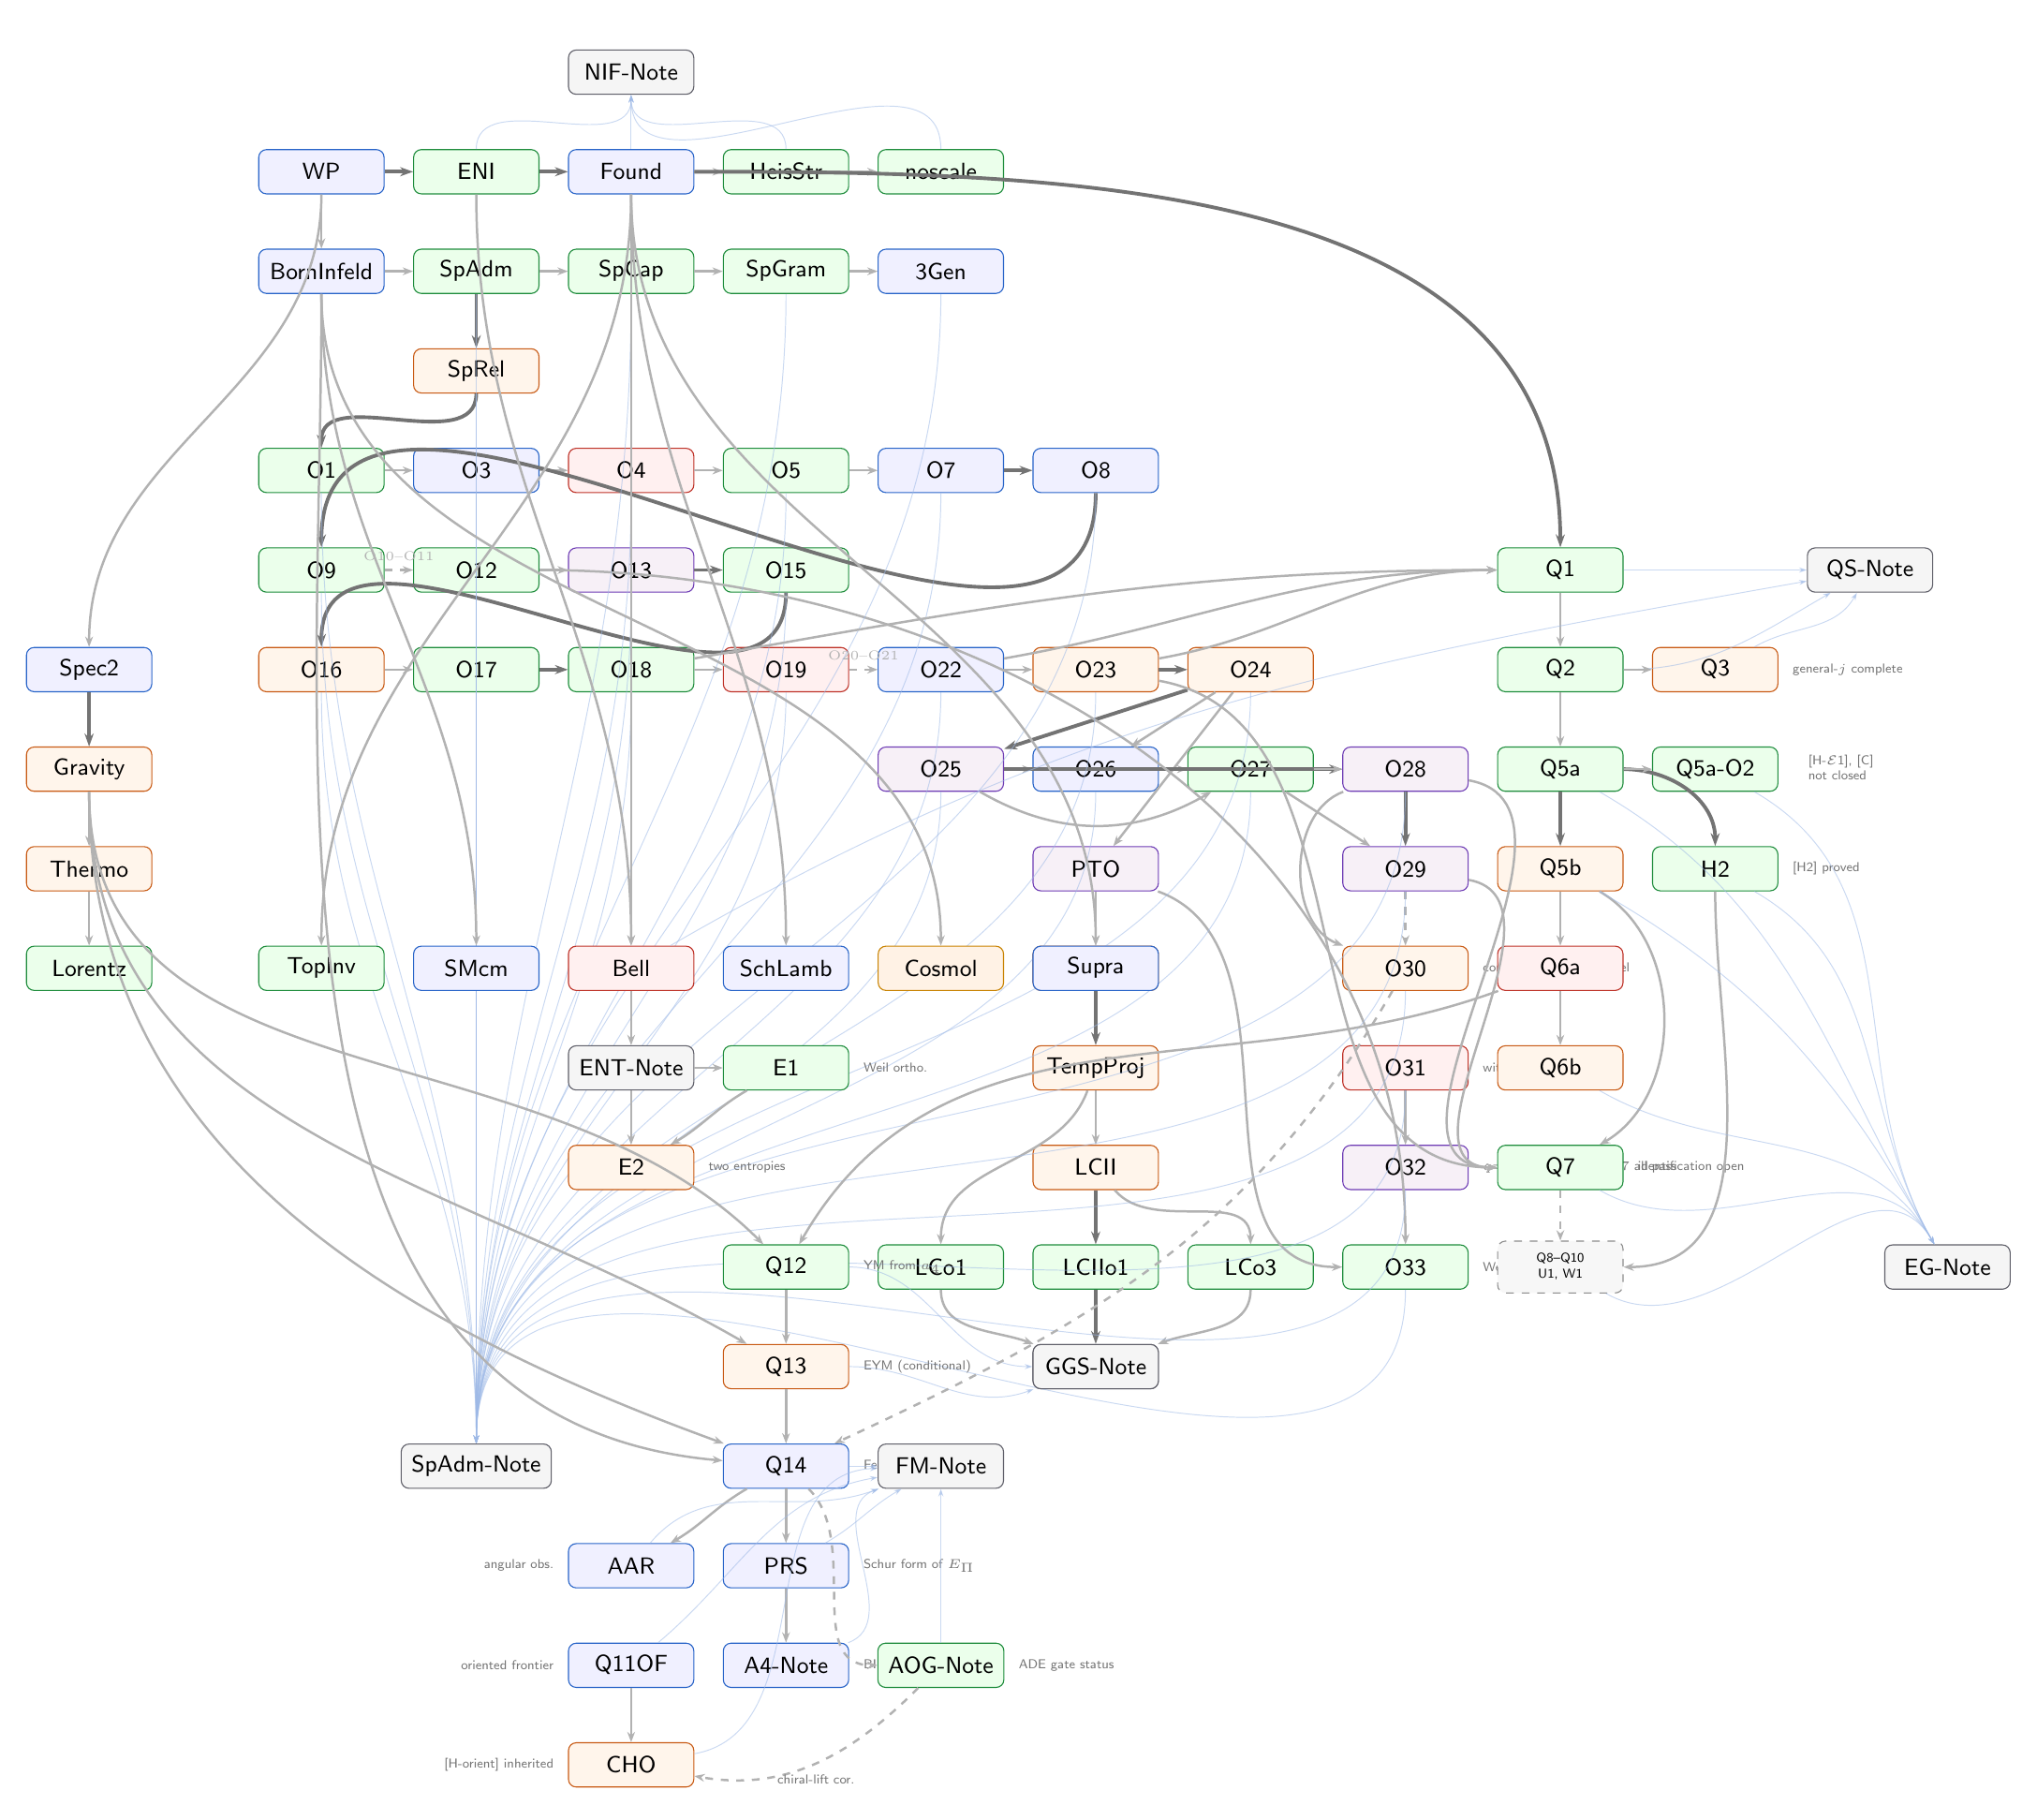
\begin{tikzpicture}[
          every node/.style={font=\small\sffamily},
          box/.style={draw, rounded corners=3pt, inner sep=4pt,
          minimum width=1.7cm, minimum height=0.6cm},
          P/.style={box, fill=green!8,  draw=cproved,  text=black},
          S/.style={box, fill=blue!6,   draw=cstruct,  text=black},
          H/.style={box, fill=orange!10,draw=cheur,    text=black},
          Oc/.style={box, fill=red!6,   draw=copen,    text=black},
          N/.style={box, fill=violet!6,  draw=cnum,     text=black},
          C/.style={box, fill=orange!8,  draw=ccond,    text=black},
          Y/.style={box, fill=gray!8,    draw=csynth,   text=black},
          arr/.style={-{Stealth[length=4pt,width=3pt]}, gray!60, line width=0.9pt},
          spine/.style={-{Stealth[length=5pt,width=3.5pt]}, black!55, line width=1.4pt},
          gather/.style={-{Stealth[length=3pt,width=2pt]}, draw=cstruct!45, line width=0.35pt, opacity=0.55},
        ]

          \newcommand{\dx}{2.1cm}
          \newcommand{\dy}{1.35cm}

          \node[S] (WP)     at (0,0)          {WP};
          \node[P] (ENI)    at (\dx,0)        {ENI};
          \node[S] (Found)  at (2*\dx,0)      {Found};
          \node[P] (Heis)   at (3*\dx,0)      {HeisStr};
          \node[P] (nos)    at (4*\dx,0)      {noscale};

          \draw[spine] (WP)--(ENI);
          \draw[spine] (ENI)--(Found);
          \draw[arr,dashed] (Found)--(Heis);
          \draw[arr]   (Found)--(nos);

          \node[S]  (BI)    at (0,-\dy)       {BornInfeld};
          \node[P]  (SpA)   at (\dx,-\dy)     {SpAdm};
          \node[P] (SpCap) at (2*\dx,-\dy)   {SpCap};
          \node[P]  (SpG)   at (3*\dx,-\dy)   {SpGram};
          \node[S]  (ThGn)  at (4*\dx,-\dy)   {3Gen};
          \node[C]  (SpR)   at (\dx,-2*\dy)   {SpRel};

          \draw[arr]   (WP)--(BI);
          \draw[arr]   (BI)--(SpA);
          \draw[arr]   (SpA)--(SpCap);
          \draw[arr]   (SpCap)--(SpG);
          \draw[arr]   (SpG)--(ThGn);
          \draw[spine] (SpA)--(SpR);

          \node[P] (O1)  at (0,-3*\dy)        {O1};
          \node[S] (O3)  at (\dx,-3*\dy)      {O3};
          \node[Oc] (O4)  at (2*\dx,-3*\dy)    {O4};
          \node[P] (O5)  at (3*\dx,-3*\dy)    {O5};
          \node[S] (O7)  at (4*\dx,-3*\dy)    {O7};
          \node[S] (O8)  at (5*\dx,-3*\dy)    {O8};

          \draw[spine] (SpR) to[out=-90,in=90] (O1);
          \draw[arr]   (O1)--(O3);
          \draw[arr]   (O3)--(O4);
          \draw[arr]   (O4)--(O5);
          \draw[arr]   (O5)--(O7);
          \draw[spine] (O7)--(O8);

          \node[P] (O9)   at (0,-4*\dy)       {O9};
          \node[P] (O12)  at (\dx,-4*\dy)     {O12};
          \node[N] (O13)  at (2*\dx,-4*\dy)   {O13};
          \node[P] (O15)  at (3*\dx,-4*\dy)   {O15};

          \draw[spine] (O8) to[out=-90,in=90] (O9);
          \draw[arr,dashed] (O9) -- node[above,font=\tiny]{O10--O11} (O12);
          \draw[arr]   (O12)--(O13);
          \draw[spine] (O13)--(O15);

          \node[C] (O16)  at (0,-5*\dy)       {O16};
          \node[P] (O17)  at (\dx,-5*\dy)     {O17};
          \node[P] (O18)  at (2*\dx,-5*\dy)   {O18};
          \node[Oc] (O19)  at (3*\dx,-5*\dy)   {O19};
          \node[S] (O22)  at (4*\dx,-5*\dy)   {O22};
          \node[C] (O23)  at (5*\dx,-5*\dy)   {O23};
          \node[C] (O24)  at (6*\dx,-5*\dy)   {O24};

          \draw[spine] (O15) to[out=-90,in=90] (O16);
          \draw[arr]   (O16)--(O17);
          \draw[spine] (O17)--(O18);
          \draw[arr]   (O18)--(O19);
          \draw[arr,dashed] (O19) -- node[above,font=\tiny]{O20--O21} (O22);
          \draw[arr]   (O22)--(O23);
          \draw[spine] (O23)--(O24);

          \node[N] (O25)  at (4*\dx,-6*\dy)   {O25};
          \node[S] (O26)  at (5*\dx,-6*\dy)   {O26};
          \node[P] (O27)  at (6*\dx,-6*\dy)   {O27};
          \node[N] (O28)  at (7*\dx,-6*\dy)   {O28};
          \node[N] (O29)  at (7*\dx,-7*\dy)   {O29};
          \node[C] (O30)  at (7*\dx,-8*\dy)   {O30};
          \node[font=\tiny\sffamily,text=black!55,right=2pt] at (O30.east)
            {conditional $3\times3$ model};
          \node[Oc] (O31)  at (7*\dx,-9*\dy)   {O31};
          \node[font=\tiny\sffamily,text=black!55,right=2pt] at (O31.east)
            {withdrawn claims};
          \node[N] (O32)  at (7*\dx,-10*\dy)  {O32};
          \node[font=\tiny\sffamily,text=black!55,right=2pt] at (O32.east)
            {$q{=}61,151,211,307$ all pass};
          \node[P] (O33)  at (7*\dx,-11*\dy)  {O33};
          \node[font=\tiny\sffamily,text=black!55,right=2pt] at (O33.east)
            {Weil doublets};
          \node[N] (PTO)    at (5*\dx,-7*\dy)   {PTO};
          \node[C] (LorCap) at (5*\dx,-8*\dy)  {LorCap};
          \node[C] (TempPr) at (5*\dx,-9*\dy)  {TempProj};
          \node[C] (LCII)   at (5*\dx,-10*\dy) {LCII};
          \node[P] (LCIIo1) at (5*\dx,-11*\dy) {LCIIo1};
          \node[P] (LCo1)   at (4*\dx,-11*\dy) {LCo1};
          \node[P] (LCo3)   at (6*\dx,-11*\dy) {LCo3};
          \node[Y] (LCsyn)  at (5*\dx,-12*\dy) {LC-Synth};

          \draw[arr]   (PTO)    -- (LorCap);
          \draw[spine] (LorCap) -- (TempPr);
          \draw[arr]   (TempPr) -- (LCII);
          \draw[spine] (LCII)   -- (LCIIo1);
          \draw[arr]   (TempPr) to[out=-110,in=90] (LCo1);
          \draw[arr]   (LCII)   to[out=-50,in=90]  (LCo3);
          \draw[spine] (LCIIo1) -- (LCsyn);
          \draw[arr]   (LCo1)   to[out=-90,in=160] (LCsyn);
          \draw[arr]   (LCo3)   to[out=-90,in=20]  (LCsyn);

          \draw[spine] (O24) -- (O25);
          \draw[arr]   (O24) -- (O26);
          \draw[arr]   (O25) -- (O26);
          \draw[arr]   (O25) to[out=-30,in=-150] (O27);
          \draw[arr]   (O28) to[out=200,in=160] (O30);
          \draw[arr]   (O31) -- (O32);
          \draw[arr]   (O26) -- (O27);
          \draw[arr]   (O24) -- (PTO);
          \draw[spine] (O25) -- (O28);
          \draw[arr]   (O27) -- (O28);
          \draw[spine] (O28) -- (O29);
          \draw[arr]   (O27) -- (O29);
          \draw[arr,dashed] (O29) -- (O30);
          \draw[arr]   (O12) to[out=0,in=90] (O33);
          \draw[arr]   (PTO) to[out=-20,in=180] (O33);

% Spectral admissibility sub-programme synthesis (presentation note):
% aggregates all constituent papers (5 precursors + O-series).
          \node[Y] (SpANote) at (\dx,-13*\dy) {SpAdm-Note};
          \foreach \n in {SpA,SpCap,SpG,ThGn,SpR,O1,O3,O4,O5,O7,O8,O9,O12,O13,O15,O16,O17,%
          O18,O19,O22,O23,O24,O25,O26,O27,O28,O29,O30,O31,O32,O33}
          \draw[gather] (\n) to[out=-90,in=90] (SpANote);

% Non-injective foundations sub-programme synthesis (presentation note 5):
% aggregates the four constituents of Branch I (ENI, Foundation, HeisStr, noscale).
          \node[Y] (NIFNote) at (2*\dx,\dy) {NIF-Note};
          \foreach \n in {ENI,Found,Heis,nos}
          \draw[gather] (\n) to[out=90,in=-90] (NIFNote);

          \node[P] (Q1)   at (8*\dx,-4*\dy)   {Q1};
          \node[P] (Q2)   at (8*\dx,-5*\dy)   {Q2};
          \node[C] (Q3)   at (9*\dx,-5*\dy)   {Q3};
          \node[font=\tiny\sffamily,text=black!55,right=2pt] at (Q3.east)
            {general-$j$ complete};

% Quantum structure sub-programme synthesis (presentation note 7):
% aggregates Q1, Q2, Q3, and the Bell paper.
          \node[Y] (QSNote) at (10*\dx,-4*\dy) {QS-Note};
          \draw[gather] (Q1)   to[out=0,in=180]  (QSNote);
          \draw[gather] (Q2)   to[out=0,in=-150] (QSNote);
          \draw[gather] (Q3)   to[out=30,in=-120] (QSNote);

          \node[P] (Q5a)  at (8*\dx,-6*\dy)   {Q5a};
          \node[P] (Q5aO2) at (9*\dx,-6*\dy)  {Q5a-O2};
          \node[C] (Q5b)  at (8*\dx,-7*\dy)   {Q5b};
          \node[Oc] (Q6a)  at (8*\dx,-8*\dy)   {Q6a};
          \node[C] (Q6b)  at (8*\dx,-9*\dy)   {Q6b};
          \node[P] (Q7)   at (8*\dx,-10*\dy)  {Q7};
          \node[font=\tiny\sffamily,text=black!55,right=2pt] at (Q7.east)
            {identification open};
          \node[box,dashed,draw=black!45,fill=black!3,font=\tiny\sffamily]
          (geom)  at (8*\dx,-11*\dy)  {\begin{tabular}{c}
                                         Q8--Q10\\U1, W1
          \end{tabular}};
          \node[P] (H2)   at (9*\dx,-7*\dy)   {H2};
          \node[font=\tiny\sffamily,text=black!55,right=2pt] at (H2.east)
            {[H2] proved};

          \draw[arr]   (Q5b)   to[out=-30,in=30]  (Q7);
          \draw[arr]   (O23)   to[out=-10,in=180] (Q7);
          \draw[arr]   (O28)   to[out=-10,in=180] (Q7);
          \draw[arr]   (O29)   to[out=-10,in=180] (Q7);
          \draw[arr,dashed]   (Q7)--(geom);
          \draw[spine] (Q5a)   to[out=0,in=90]   (H2);
          \draw[arr]   (H2)    to[out=-90,in=0]  (geom);

% Emergent geometry sub-programme synthesis (presentation note):
% aggregates the geometric emergence papers (Q5a, Q5a-O2, Q5b, Q6b, Q7, H2,
% and the Q8--Q10/U1/W1 block).
          \node[Y] (EGNote) at (10.5*\dx,-11*\dy) {EG-Note};
          \foreach \n in {Q5a,Q5aO2,Q5b,Q6b,Q7,H2,geom}
          \draw[gather] (\n) to[out=-30,in=120] (EGNote);

          \draw[spine] (Found) to[out=0,in=90] (Q1);
          \draw[arr]   (O18)   to[out=10,in=180] (Q1);
          \draw[arr]   (O22)   to[out=10,in=180] (Q1);
          \draw[arr]   (O23)   to[out=10,in=180] (Q1);
          \draw[arr]   (Q1)--(Q2);
          \draw[arr]   (Q2)--(Q3);
          \draw[arr]   (Q2)--(Q5a);
          \draw[arr]   (Q5a)--(Q5aO2);
          \node[font=\tiny\sffamily,text=black!55,right=2pt] at (Q5aO2.east)
            {\begin{tabular}{l}[H-$\mathcal{E}$1], [C]\\not closed
          \end{tabular}};
          \draw[spine] (Q5a)--(Q5b);
          \draw[arr]   (Q5b)--(Q6a);
          % O31 no longer supplies the former SU(3) derivation edge to Q6a.
          \draw[arr]   (Q6a)--(Q6b);

          \node[S] (Sp2)  at (-1.5*\dx,-5*\dy) {Spec2};
          \node[C] (Grav) at (-1.5*\dx,-6*\dy) {Gravity};
          \node[C] (Thm)  at (-1.5*\dx,-7*\dy) {Thermo};
          \node[P] (Lor)  at (-1.5*\dx,-8*\dy) {Lorentz};

          \draw[arr]   (WP) to[out=-90,in=90] (Sp2);
          \draw[spine] (Sp2)--(Grav);
          \draw[arr]   (Grav)--(Thm);
          \draw[arr]   (Thm)--(Lor);

          \node[P] (TopI) at (0,-8*\dy)        {TopInv};
          \node[S] (SMcm) at (\dx,-8*\dy)      {SMcm};
          \node[Oc] (Bell) at (2*\dx,-8*\dy)   {Bell};
          \node[S] (Schw) at (3*\dx,-8*\dy)    {SchLamb};
          \node[H] (Cosm) at (4*\dx,-8*\dy)    {Cosmol};
          \node[S] (Supra)at (5*\dx,-8*\dy)    {Supra};

          \draw[arr] (Found) to[out=-90,in=90] (TopI);
          \draw[arr] (BI)    to[out=-90,in=90] (SMcm);
          \draw[arr] (Found) to[out=-90,in=90] (Bell);
          \draw[arr] (ENI)   to[out=-90,in=90] (Bell);
          \draw[arr] (Found) to[out=-90,in=90] (Schw);
          \draw[arr] (BI)    to[out=-90,in=90] (Cosm);
          \draw[arr] (Found) to[out=-90,in=90] (Supra);

          \node[Y] (ENTn) at (2*\dx,-9*\dy)    {ENT-Note};
          \draw[arr] (Bell) to[out=-90,in=90] (ENTn);
          \draw[gather] (Bell) to[out=30,in=-170] (QSNote);

          \node[P] (ENTe1) at (3*\dx,-9*\dy)   {E1};
          \node[font=\tiny\sffamily,text=black!55,right=2pt] at (ENTe1.east)
            {Weil ortho.};
          \draw[arr] (ENTn) to[out=0,in=180] (ENTe1);

          \node[C] (ENTe2) at (2*\dx,-10*\dy)  {E2};
          \node[font=\tiny\sffamily,text=black!55,right=2pt] at (ENTe2.east)
            {two entropies};
          \draw[arr] (ENTn)  to[out=-90,in=90] (ENTe2);
          \draw[arr] (ENTe1) to[out=-150,in=30] (ENTe2);

          \node[P] (Q12) at (3*\dx,-11*\dy) {Q12};
          \node[font=\tiny\sffamily,text=black!55,right=2pt] at (Q12.east)
            {YM from $a_4$};
          \draw[arr] (Grav) to[out=-90,in=135] (Q12);
          \draw[arr] (Q6a)  to[out=200,in=60]  (Q12);

          \node[C] (Q13) at (3*\dx,-12*\dy) {Q13};
          \node[font=\tiny\sffamily,text=black!55,right=2pt] at (Q13.east)
            {EYM (conditional)};
          \draw[arr] (Q12)  to[out=-90,in=90]  (Q13);
          \draw[arr] (Grav) to[out=-90,in=150] (Q13);

% Gauge-gravity stratification sub-programme synthesis (presentation note 8):
% aggregates Q12 and Q13.
          \node[Y] (GGSNote) at (5*\dx,-12*\dy) {GGS-Note};
          \draw[gather] (Q12) to[out=0,in=180] (GGSNote);
          \draw[gather] (Q13) to[out=0,in=200] (GGSNote);

          \node[S] (Q14) at (3*\dx,-13*\dy) {Q14};
          \node[font=\tiny\sffamily,text=black!55,right=2pt] at (Q14.east)
            {Fermions + chirality};
          \draw[arr] (Q13) to[out=-90,in=90]  (Q14);
          \draw[arr] (Grav) to[out=-90,in=160] (Q14);
          \draw[arr] (BI)   to[out=-90,in=175] (Q14);
          \draw[arr,dashed] (O30) to[out=-120,in=25]  (Q14);

          \node[S] (PRS) at (3*\dx,-14*\dy) {PRS};
          \node[font=\tiny\sffamily,text=black!55,right=2pt] at (PRS.east)
            {Schur form of $E_\Pi$};
          \draw[arr] (Q14) to[out=-90,in=90]  (PRS);

          \node[S] (AAR) at (2*\dx,-14*\dy) {AAR};
          \node[font=\tiny\sffamily,text=black!55,left=2pt] at (AAR.west)
            {angular obs.};
          \draw[arr] (Q14) to[out=-150,in=30]  (AAR);

          \node[S] (Q11OF) at (2*\dx,-15*\dy) {Q11OF};
          \node[font=\tiny\sffamily,text=black!55,left=2pt] at (Q11OF.west)
            {oriented frontier};

          \node[C] (CHO) at (2*\dx,-16*\dy) {CHO};
          \node[font=\tiny\sffamily,text=black!55,left=2pt] at (CHO.west)
            {[H-orient] inherited};
          \draw[arr] (Q11OF) to[out=-90,in=90]  (CHO);

          \node[S] (A4Note) at (3*\dx,-15*\dy) {A4-Note};
          \node[font=\tiny\sffamily,text=black!55,right=2pt] at (A4Note.east)
            {BI saturation margin};
          \draw[arr] (PRS) to[out=-90,in=90]  (A4Note);

          \node[P] (AOG) at (4*\dx,-15*\dy) {AOG-Note};
          \node[font=\tiny\sffamily,text=black!55,right=2pt] at (AOG.east)
            {ADE gate status};
          \draw[arr,dashed] (Q14) to[out=-45,in=180] (AOG);
          \draw[arr,dashed] (AOG) to[out=-135,in=-10]
            node[font=\tiny\sffamily,text=black!55,below=1pt,midway] {chiral-lift cor.} (CHO);

% Fermionic matter sub-programme synthesis (presentation note 6):
% aggregates Q14, PRS, AAR, Q11OF, A4-Note and AOG-Note.
          \node[Y] (FMNote) at (4*\dx,-13*\dy) {FM-Note};
          \draw[gather] (Q14)    to[out=0,in=180]   (FMNote);
          \draw[gather] (PRS)    to[out=30,in=-150] (FMNote);
          \draw[gather] (AAR)    to[out=50,in=-160] (FMNote);
          \draw[gather] (Q11OF)  to[out=40,in=-170] (FMNote);
          \draw[gather] (A4Note) to[out=20,in=-160] (FMNote);
          \draw[gather] (AOG)    to[out=90,in=-90]  (FMNote);
          \draw[gather] (CHO)    to[out=10,in=-178] (FMNote);

        \end{tikzpicture}
      }
      \caption{Logical dependency DAG of the Cosmochrony programme.
      Colour coding: \textcolor{cproved}{$\blacksquare$}~\sproved{},
        \textcolor{cstruct}{$\blacksquare$}~\sstruct{},
        \textcolor{cnum}{$\blacksquare$}~\snum{},
        \textcolor{ccond}{$\blacksquare$}~\scond{},
        \textcolor{cheur}{$\blacksquare$}~\sheur{},
        \textcolor{copen}{$\blacksquare$}~\sopen{},
        \textcolor{csynth}{$\blacksquare$}~\ssynth{}; each single-paper node carries the primary label of its
        inventory row, while the dashed composite block gathers a sub-chain and carries no paper label.
        In both figures the grey side annotations and the dashed result boxes carry no status colour: where their
        text states a status it is that of the component named, not the primary label of the node.
        The interactive graph's conditional-reading and postulated
        edges (EG-Note to Q12, Q13 and Q14) are not drawn in this figure.
        Thick arrows indicate the main logical spine; thin arrows indicate supporting dependencies.
        Dashed arrows with labels abbreviate linear sub-chains.
        The faint converging edges gather the constituent papers of each thematic sub-programme into
        its synthesis node: the Branch~I foundational papers (ENI, Foundation, HeisStr, noscale) into
        \textbf{NIF-Note}, the spectral admissibility papers into \textbf{SpAdm-Note}, the
        Lorentz-capacity papers into \textbf{LC-Synth}, the geometric emergence papers into
        \textbf{EG-Note}, Q1/Q2/Q3 and the Bell paper into the quantum-structure
        \textbf{QS-Note}, Q12 and Q13 into the gauge--gravity stratification
        \textbf{GGS-Note}, and Q14 with the companion notes PRS, AAR, Q11OF, CHO, A4-Note and AOG-Note into the
        fermionic-matter \textbf{FM-Note}.
        The dashed uncoloured arrow from Q7 leads to the geometric emergence block Q8--Q10, U1 and
        W1, detailed in Figure~\ref{fig:geom}; it carries no status colour because what Q7
        version~2.0 supplies forward is conditional on an identification its own inventory row
        records as open.
        The interactive version with clickable nodes is provided as a companion HTML file.}
      \label{fig:dag}
    \end{figure}

    \clearpage

    \begin{figure}[p]
      \centering
      \resizebox{\textwidth}{!}{%
        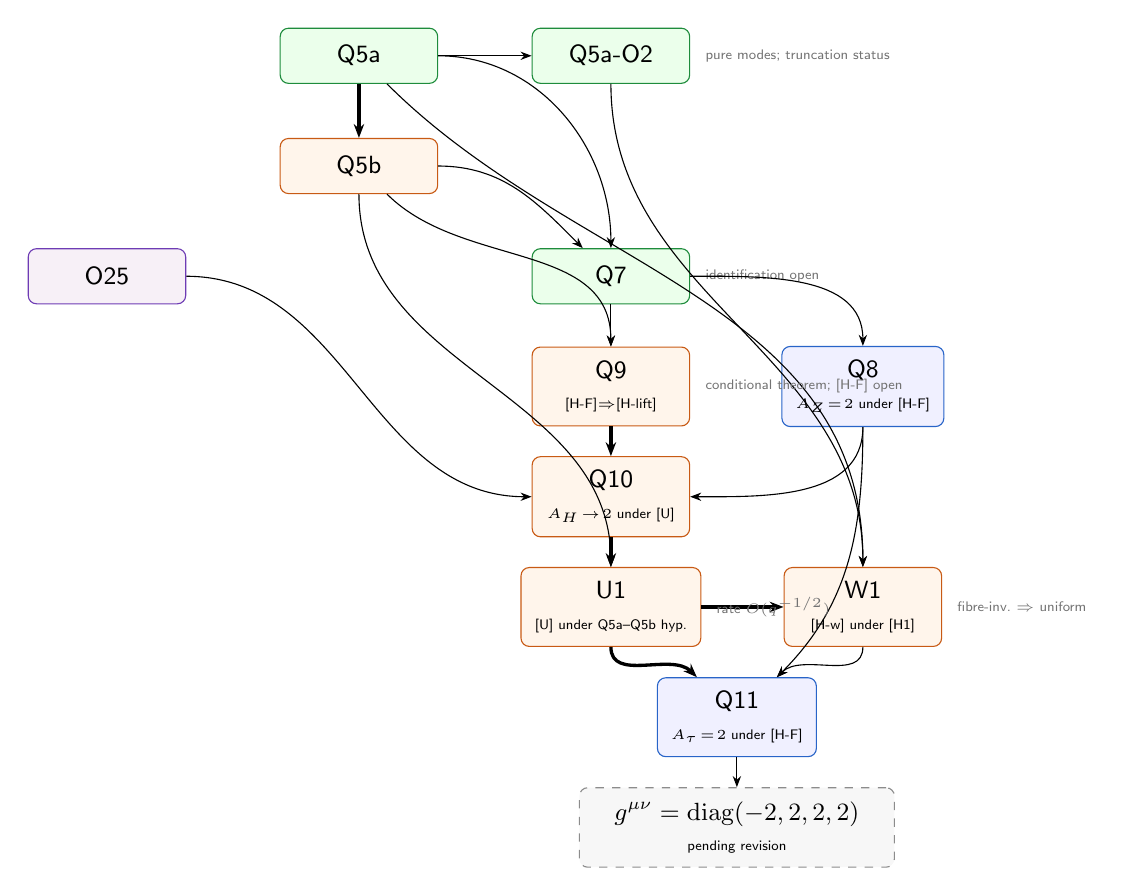
\begin{tikzpicture}[
          every node/.style={font=\small\sffamily},
          box/.style={draw, rounded corners=3pt, inner sep=5pt,
          minimum width=2.0cm, minimum height=0.7cm, align=center},
          P/.style={box, fill=green!8,  draw=cproved,  text=black},
          S/.style={box, fill=blue!6,   draw=cstruct,  text=black},
          N/.style={box, fill=violet!6,  draw=cnum,     text=black},
          C/.style={box, fill=orange!8,  draw=ccond,    text=black},
          spine/.style={-{Stealth[length=5pt]}, line width=1.2pt},
          arr/.style={-{Stealth[length=4pt]}, thin},
        ]

          \def\dx{3.2cm}
          \def\dy{1.4cm}

          % ── Inputs (left column) ──────────────────────────────
          \node[P] (Q5a)   at (0,0)          {Q5a};
          \node[P] (Q5aO2) at (\dx,0)        {Q5a-O2};
          \node[C] (Q5b)   at (0,-\dy)       {Q5b};
          \node[N] (O25)   at (-\dx,-2*\dy)  {O25};

          % ── Core chain (centre column) ───────────────────────
          \node[P] (Q7)  at (\dx,-2*\dy) {Q7};
          \node[font=\tiny\sffamily,text=black!55,right=2pt] at (Q7.east)
            {identification open};
          \node[S] (Q8)  at (2*\dx,-3*\dy){Q8\\{\tiny $A_Z\!=\!2$ under [H-F]}};
          \node[C] (Q9)  at (\dx,-3*\dy) {Q9\\{\tiny [H-F]$\Rightarrow$[H-lift]}};
          \node[C] (Q10) at (\dx,-4*\dy) {Q10\\{\tiny $A_H\!\to\!2$ under [U]}};
          \node[C] (U1)  at (\dx,-5*\dy) {U1\\{\tiny [U] under Q5a--Q5b hyp.}};
          \node[C] (W1)  at (2*\dx,-5*\dy){W1\\{\tiny [H-w] under [H1]}};

          % Q11 and final result
          \node[S] (Q11) at (\dx+0.5*\dx,-6*\dy)
            {Q11\\{\tiny $A_\tau\!=\!2$ under [H-F]}};
          \node[box,dashed,draw=black!45,fill=black!3,minimum width=4cm] (Met)
          at (\dx+0.5*\dx,-7*\dy)
            {$g^{\mu\nu}=\mathrm{diag}(-2,2,2,2)$\\{\tiny pending revision}};

          % ── Edges ────────────────────────────────────────────
          \draw[arr]   (Q5a)--(Q5aO2);
          \draw[spine] (Q5a)--(Q5b);
          \draw[arr]   (Q5a) to[out=0,in=90] (Q7);
          \draw[arr]   (Q5aO2) to[out=-90,in=90] (W1);
          \draw[arr]   (Q5b) to[out=0,in=135] (Q7);
          \draw[arr]   (Q5b) to[out=-45,in=90] (Q9);
          \draw[arr]   (Q5b) to[out=-90,in=90] (U1);
          \draw[arr]   (O25) to[out=0,in=180] (Q10);

          \draw[arr]   (Q7)--(Q9);
          \draw[arr]   (Q7) to[out=0,in=90] (Q8);
          \draw[spine] (Q9)--(Q10);
          \draw[arr]   (Q8) to[out=-90,in=0] (Q10);
          \draw[spine] (Q10)--(U1);
          \draw[spine] (U1)--(W1);
          \draw[arr]   (Q5a) to[out=-45,in=90] (W1);

          \draw[spine] (U1)  to[out=-90,in=135] (Q11);
          \draw[arr]   (Q8)  to[out=-90,in=45]  (Q11);
          \draw[arr]   (W1)  to[out=-90,in=45]  (Q11);
          \draw[arr]   (Q11) -- (Met);

          % ── Status annotations ───────────────────────────────
          \node[font=\tiny\sffamily,text=black!55,right=2pt] at (Q5aO2.east)
            {pure modes; truncation status};
          \node[font=\tiny\sffamily,text=black!55,right=2pt] at (Q9.east)
            {conditional theorem; [H-F] open};
          \node[font=\tiny\sffamily,text=black!55,right=2pt] at (U1.east)
            {rate $O(q^{-1/2})$};
          \node[font=\tiny\sffamily,text=black!55,right=2pt] at (W1.east)
            {fibre-inv.\ $\Rightarrow$ uniform};

        \end{tikzpicture}
      }
      \caption{Geometric emergence sub-programme: logical chain from Q5a to the effective
      Lorentzian co-metric.
      \textbf{Q5a-O2}~\cite{Beau2026q5ao2}~(\sproved{} for its stated results): pure Fourier
      modes of the pre-saturation pipeline; truncation status of the three-coordinate reduction;
      rules out the $q^{-1}$ coercivity scale; [H-$\mathcal{E}$1] and [C] are not closed by a
      finite-rank route (zero-form limit on the canonical filtration, Q5a version 3.2).
      \textbf{Q9}~(\scond{} on [H-F]; the implication itself is \sproved): under the frozen, unestablished
        hypothesis [H-F], the modulation-sector position-energy form contribution satisfies
        $\mathcal{E}^X_q(f_q)\leq C/q$ along recovery sequences; hence
        [H-F] $\Rightarrow$ [H-lift] and coercivity gives $A_H>0$ under [H-F].
        \textbf{Q8}~(\sstruct{}, within the frozen [H-F]; pending revision): $A_Z = C_{\mathfrak{su}(2)} = 2$
        by Casimir rigidity; normalisation fixed by horizontal sector.
        \textbf{Q10}~(\scond{} on~[U]; pending revision): universality~[U] $\Rightarrow$
        $\mathfrak{su}(2)$-isotropy $\Rightarrow$ $A_H \to 2$.
        \textbf{U1}~(\scond{} on the Q5a--Q5b hypotheses): [U] with rate $O(q^{-1/2})$ from Weil-generator
        Lipschitz bound and BFS--Carnot--Carath\'eodory convergence (Q5b).
        \textbf{W1}~(\scond{} on [H1]): [H-w] as a structural consequence of fibre-invariance
        ($\mathcal{O}=\mathrm{Im}\,\Pi$), quantitative control from~U1.
        The metric reading of
        $g^{\mu\nu} = \mathrm{diag}(-A_\tau,2,2,2)$ remains conditional on the independent,
        unestablished spatial-limit hypothesis [H-L] of Q5a version 3.2/Q5b version 2.1, and on the
        identification of the measured admissible space with the spin-$1$ module, which Q7
        version~2.0 records as supplied by no paper: Q7 is \sproved{} for the requirements it states on the
        supplied carrier and \sopen{} for that identification.
        [H-F] is also unestablished.}
      \label{fig:geom}
    \end{figure}
    \label{sec:inventory}

    Table~\ref{tab:inventory} lists all 116 papers of the programme, the present registry excepted.
    The \textbf{Key} column gives the citation key used in
    \texttt{cosmochrony-bibliography}.
    The final block gathers the sub-programme presentation and synthesis notes, marked
    \ssynth{}: they organise results established elsewhere and are not themselves sources of new
    results.

    \setlength\LTleft{0pt}
    \setlength\LTright{0pt}
    \begin{longtable}{@{}p{1.70cm}p{2.9cm}p{1.3cm}p{6.25cm}>{\raggedright\arraybackslash}p{2.0cm}@{}}
      \caption{Complete inventory of the 116 programme papers, excluding the present registry.}
      \label{tab:inventory}\\
      \toprule
      \textbf{Label} & \textbf{Short title} & \textbf{Key} & \textbf{Main contribution} & \textbf{Status}\\
      \midrule
      \endfirsthead
      \toprule
      \textbf{Label} & \textbf{Short title} & \textbf{Key} & \textbf{Main contribution} & \textbf{Status}\\
      \midrule
      \endhead
      \midrule\multicolumn{5}{r}{\small\itshape continued\ldots}\\\midrule
      \endfoot
      \bottomrule
      \endlastfoot
      WP & White Paper & \cite{Cosmochrony} &
      Programme overview; substrate~$\chi$; iterated projection; BI constraint; relaxation cascade &
      \sstruct \\[3pt]
      ENI & Emergence \& non-injectivity & \cite{Beau2026l} &
      No-go: genuine emergence $\Leftrightarrow$ $\Pi$ non-injective; projection entropy $S_\Pi$ &
      \sproved \\[3pt]
      Found & Foundation & \cite{Beau2026m} &
      Axioms A1--A4; the published Heisenberg/Weil selection theorem is not established;
      version 2.2: continuum-limit passages conditioned on the unestablished spatial-limit hypothesis
      [H-L] (Q5b version 2.0); co-metric completion conditional on [H-L]; relation to HJ, symplectic, WKB, FRG
      formalisms &
      \sstruct\ /\ \scond{} on [H-L]\ /\ \sopen \\[3pt]
      HeisStr & Heisenberg carrier obstruction & \cite{Beau2026HeisenbergStructure} &
      Contains the explicit \(S_3\) countermodel to the carrier-selection
      implication and corrects the central-subgroup/Schur step (version 2.1); the conditional Stone--von Neumann
      endpoint remains valid when the Heisenberg carrier and central character are supplied &
      \sproved\ /\ \scond{} on a supplied carrier and central character\ /\ \sopen \\[3pt]
      noscale & No external scale & \cite{Beau2026j} &
      No independent dimensional parameter beyond $c_{\mathrm{BI}}$ &
      \sproved \\[3pt]
      EffComp & Effective composition prerequisites (K4) & \cite{Beau2026esub} &
      Independence blocks $=$ bicliques of the projected support; full simplex lifts all products;
      cylindrical-conditioning closure iff $\operatorname{rank} W = 1$; support rectangularity does not imply
      preparation independence; contract proposed, not derived from A1--A4 &
      \sproved\ /\ \sopen \\[3pt]
      STEFT & Simplicial states \& local tomography (K4 cont'd) & \cite{Beau2026steft} &
      Primitive family never convex ($m\geq2$, unconditional); classical randomisation $P1$ closes it
      rank-independently; affine effects $=$ cube (representation, not availability); coarse-graining gives
      the Boolean skeleton, $\mathrm{AX\text{-}RND}$ the full cube; $P1$/$\mathrm{AX\text{-}RND}$ independent, unified
      only under an explicit control-independence clause; pointwise product forced given composed-effect
      existence; local tomography iff local families span their ambient spaces &
      \sproved \\[3pt]
      HMPL & Power-lift refinement obstruction (STEFT cont'd) & \cite{Beau2026hmpl} &
      $\mu^\alpha$ Kolmogorov-consistent iff $\alpha=1$ (general, self-contained); escort renormalisation
      restores it trivially but departs from the pointwise lift; exact $\mathbb{Q}(\sqrt2)$ instantiation
      under its own postulate H2 on the TrajectoryBranching automaton, distinct from the Q5a [H2]; endpoint/shadow
      quotients incomparable;
      $X\leftrightarrow X^{-1}$ transports the endpoint by an exact automorphism, forcing real co-$b_n$
      phase sums; bounded exact search finds no cancellation among $62$ nontrivial-phase classes of $64$ &
      \sproved\ /\ \scond{} on its postulate H2 for the instantiation \\[3pt]
      \midrule
      Born\-Infeld & Bounded relational capacity & \cite{Beau2026c} &
      Capacity axiom [A-cap]; BI action as saturation candidate; bridges open &
      \sstruct\ /\ \sopen \\[3pt]
      SpAdm & Spectral admissibility ($Q_8$) & \cite{Beau2026a1} &
      $A^{\max}_n = c_{\mathrm{BI}}/\sqrt{\lambda_n}$; first tractable instance &
      \sproved \\[3pt]
      SpCap & Spectral capacity & \cite{Beau2026a2} &
      Capacity functional $\mathcal{C}(G,S)$; binary-polyhedral maximality proved via
      adjoint identity $\hat{A}_{\mathrm{adj}} = 2M - I$ and icosahedral isotropy &
      \sproved \\[3pt]
      SpGram & Gram rigidity & \cite{Beau2026a3} &
      Neutral-generator geometry from $G_{st} = -\tfrac{1}{2}\chi_\rho(st)$ &
      \sproved \\[3pt]
      3Gen & Three generations & \cite{Beau2026a4} &
      Three-generation structure from ADE stratigraphic levels &
      \sstruct \\[3pt]
      SpRel & Spectral relaxation & \cite{Beau2026a5} &
      $\Lambda_{\mathrm{proj}} \asymp \lambda_2$ for LPS expander families &
      \scond{} on the capacity--isoperimetry closure and spectral-isoperimetric saturation hypotheses \\[3pt]
      \midrule
      O1 & Variable-valence graphs & \cite{Beau2026a6} &
      LPS saturation is a fixed-valence artefact; growing valence restores window &
      \sproved \\[3pt]
      O3 & Mass hierarchy & \cite{Beau2026a7} &
      First SM connection: $\beta^* \in (0.09, 0.13)$ from lepton mass ratios &
      \sstruct \\[3pt]
      O4 & No cascade-exponent bound from bounded flux & \cite{Beau2026a8} &
      Bounded relational flux and Ramanujan expansion do not yet yield a cascade-exponent bound: the
      former derivation of $\beta \leq 1$ does not follow from the stated argument, and any structural
      upper bound on $\beta$ by this route is open &
      \sopen \\[3pt]
      O5 & Rep-theoretic obstruction & \cite{Beau2026a9} &
      Fixed-repr.\ approaches cannot close the $\beta$ gap &
      \sproved \\[3pt]
      O6 & Matrix redundancy & \cite{Beau2026a10} &
      Matrix-level dynamic redundancy: $R_n \to 0$ for the Steinberg fingerprint (proved); the
      confinement corollary $\beta_{\mathrm{eff}} \in \beta^*$ is conditional on a power-law Ansatz that
      the paper's own fingerprint does not satisfy, so a genuine power-law regime remains open &
      \sproved\ /\ \scond{} on the power-law Ansatz\ /\ \sopen \\[3pt]
      O7 & Continuum target & \cite{Beau2026a11} &
      Target: $\delta \in [7.4, 10.6]$ on 3-step fingerprints &
      \sstruct \\[3pt]
      O8 & LPS geometric obstruction & \cite{Beau2026a12} &
      Exponential shell growth $\Rightarrow$ usable window $= O(\log q)$ BFS steps, on a shell-growth
      premise the paper records as an empirical observation for its family &
      \sstruct\ /\ \snum \\[3pt]
      \midrule
      O9 & Heisenberg graphs & \cite{Beau2026a13} &
      Structural transition: $\Heis_3(\mathbb{Z}/q\mathbb{Z})$ with $|B_n| \sim n^4$ replaces LPS &
      \sproved \\[3pt]
      O10 & Large-$q$ computation & \cite{Beau2026a14} &
      Ball growth $\hat D = 3.05$ at $q=101$, continuing the convergence toward
      $D_{\mathrm{hom}} = 4$; TensorSketch obstruction identified &
      \snum \\[3pt]
      O11 & Fourier-character proxy & \cite{Beau2026a15} &
      Bidimensional proxy overcomes TensorSketch obstruction &
      \snum \\[3pt]
      O12 & Exact Weil blocks & \cite{Beau2026a16} &
      $\delta_{\mathrm{exact}}=3$ exactly (unfolded, $q\to\infty$); finite-$q$ fitted slopes are
      crossover statistics, independent of the central coordinate $\gamma$ &
      \sproved \\[3pt]
      O13 & Extended prime range & \cite{Beau2026a17} &
      Exponent sequence at $q\in\{29,61,101,151,211\}$ does not drift toward the
      phenomenological target; consistent with $\delta_{\mathrm{exact}}=3$ &
      \snum \\[3pt]
      O14 & Observable-class mismatch & \cite{Beau2026a18} &
      Fixed-$q$ normalisation $q^{-\eta}$ changes intercepts, not intra-$q$ slopes, and defines no endpoint
      correction from a fitted slope alone; the central-phase correction vanishes identically; no inter-$q$
      estimator or $\beta^*$ diagnostic follows; SGN places the shell factor additively &
      \sstruct \\[3pt]
      O15 & Block-level no-go & \cite{Beau2026a19} &
      $\beta^*=1/(\delta+\tfrac12)$ does not transfer to the exact-block setting; aggregation
      bound $\alpha_{\mathrm{dyn}}\leq\hat\delta_{\mathrm{exact}}$ holds conditionally, verified
      at $q=151,211$ &
      \sproved\ /\ \scond{} on the stated aggregation hypothesis \\[3pt]
      \midrule
      O16 & Pair observable & \cite{Beau2026a20} &
      Conjugate pairs $\{c,q-c\}$ are fibres of $\Pi$ under two independent open hypotheses;
      exponent doubling $\delta_{\mathrm{pair}}=2\delta_c$ holds conditionally, trivially on
      the real pipeline &
      \scond{} on the parity and realisation hypotheses \\[3pt]
      O17 & Block-independence, toy model & \cite{Beau2026a21} &
      Raw Gram-Schmidt redundancy is exactly independent of block parameters for any two
      blocks, not only conjugate ones; scoped to a scalar toy model, not shown for the real
      pipeline &
      \sproved \\[3pt]
      O18 & BI action parity & \cite{Beau2026a22} &
      $S_{\mathrm{BI}}[-\chi]=S_{\mathrm{BI}}[\chi]$; neither $\Pi(\chi)=\Pi(-\chi)$ nor
      the character pairing $c\leftrightarrow q-c$ follows &
      \sproved\ /\ \sopen \\[3pt]
      O19 & Proposed canonical normalisation & \cite{Beau2026a23} &
      Generic Gram--Schmidt identities survive; the residual factor, completed tests, and
      pipeline-independent observable are not established for the real pipeline, the conjugate-block identity
      of O16~\cite{Beau2026a20} forcing $r(c,q)\equiv1$ exactly on the O12/O13 exact block observable &
      \sopen\ /\ \sproved \\[3pt]
      O20 & Conditional persistence template & \cite{Beau2026a24} &
      Threshold-crossing algebra under explicit hypotheses; no intrinsic threshold or selected
      exponent window &
      \scond{} on the monotone-amplitude and capacity-bound hypotheses \\[3pt]
      O21 & Local crossing diagnostic & \cite{Beau2026a25} &
      Two-point crossing formula under a fixed normalisation; it scales under amplitude
      rescaling, while shell alignment and the capacity-to-rate carrier remain open &
      \scond{} on the shell-alignment conjecture and the cross-substrate identification\ /\ \sopen \\[3pt]
      O22 & Projection locking & \cite{Beau2026a26} &
      BI projection locking forces the O21-defined $n_3^{\mathrm{obs}}$ onto a BFS shell
      within the stated model, on a sketch-level continuous decay law and the observable-space shell
      decomposition; this does not make that rank amplitude-invariant &
      \sstruct\ /\ \sopen \\[3pt]
      O23 & Conditional adjoint dimension & \cite{Beau2026a27} &
      For a supplied irreducible $\mathbb{C}^2$ carrier, the traceless neutral sector is
      $\mathfrak{su}(2)\cong\mathrm{Im}\,\mathbb{H}$, dimension three; $Q_8$'s two-axis neutral
      generating set rules out generator-axis counting; carrier selection and the
      $\Sigma_c$-identification are open, so $\Sigma_c(n_3)=3$ is a supplied selection rule &
      \scond{} on the supplied carrier and the $\Sigma_c$ selection rule\ /\ \sopen \\[3pt]
      O24 & Observable rank rigidity & \cite{Beau2026a28} &
      Verticality Lemma develops $c_{\mathrm{BI}} \to \delta_{\mathrm{pair}}$ under the stated
      fibre hypotheses; no first-principles fibre identification and no native derivation of
      $\delta_{\mathrm{pair}} \to \beta^*$ &
      \scond{} on the supplied fibre and rank-three hypotheses\ /\ \sopen \\[3pt]
      \midrule
      O25 & Numerical campaign (extended to $q=601$) & \cite{Beau2026a29} &
      Exhaustive pair sampling through $q=211$; representative sampling of 24 pairs at $q=307$
      and 12 at $q=401,601$; raw $\delta_{\mathrm{global}} \to 7.61$ at $q=601$ under the frozen
      $\log(n+1)$ estimator; fixed-$q$ pair concentration; O14 correction overcorrects at large $q$;
      $\delta_\infty$ not pinned; reciprocal image $0.108\text{--}0.123$ only as a
      phenomenological comparison &
      \snum \\[3pt]
      O26 & Quadratic completion & \cite{Beau2026a30} &
      Dictionary: Weil blocks $\leftrightarrow$ rank-1 matrices in $M_2(\mathbb{C})$;
      connects $\Heis_3$ to $2I \subset \SU(2)$; pair-sector fibre structure taken as a motivated
      hypothesis; Level~I growth-exponent identification of $\sigma_{\mathrm{pair}}$ with a
      Hilbert--Schmidt trajectory norm proved; Level~II a conjecture ($n$-independence of the
      proportionality open); Level~III conditional on the admissible embedding $\Phi_{q,\rho}$,
      version 2.1 proves the symmetric-square rank bound under Hypothesis~4.4(a)
      (at most three for $d_\rho=2$, excluding the rank-four target under that contract);
      measured $H_{\mathrm{eff}}$ ranks do not test the embedded covariance; no rate equation follows &
      \sstruct\ /\ \scond{} on the admissible embedding\ /\ \sopen \\[3pt]
      O27 & Quaternionic rigidity & \cite{Beau2026a31} &
      Quotient factorisation does not imply equivariance; under explicit saturation,
      carrier, parity and equivariance inputs, the Schur-level counts are proved; canonical
      equivariant vector lift and any $\beta^*$ interpretation remain open &
      \sproved\ /\ \sopen \\[3pt]
      O28 & Window calibration \& $r_{\mathrm{eff}}$ & \cite{Beau2026a32} &
      Calibrated linear extrapolation of $n_1$ fails out of sample (to $q=601$, up to $+88\%$);
      the declared adjustment $\delta_{\mathrm{corr}}$ lies in $[7.4, 10.6]$ over $q \le 211$ and, by O14,
      does not correct the intra-$q$ fitted exponent (a diagnostic, not a corrected exponent); O28 reports the
      $1\%$ threshold rank $r_{\mathrm{eff}}^{1\%}=3$ and the resolved spectrum
      $[1:\tfrac{1}{2}:\tfrac{1}{2}]$ in its stated perimeter; O29's extended recomputation finds
      rank three modal rather than invariant ($32/50$ pairs at $q=101$, $103/105$ at $q=211$) &
      \snum \\[3pt]
      CC-Note & Inverse-square coverage \& constant depth & \cite{Beau2026ccnote} &
      Fingerprints are Fourier characters, so $r_c(n)=|T'_c+C\,I_{n+1}|$ with shellwise ceiling
      $18$; deterministically $n_1(q)\le22$ and $x_1(q)\asymp q^{-2}$ for $q\ge311$; under generic
      sampling $n_1(q)\to22$ and $q^2x_1(q)\to99{,}689$; O28's depths are the transitional regime &
      \sproved \\[3pt]
      SGN & Native span growth and transfer no-go & \cite{Beau2026sgn} &
      $\Delta r=\sigma_c|S_n|$; real-weight three-branch theorem and rigorous integer-rank
      finite-window law; corpus-native valence--exploration, frontier, pair-carrier and exponent-coordinate
      obstructions
      refute a Heisenberg derivation of $1/(\delta_{\mathrm{pair}}+\tfrac12)$ &
      \sproved \\[3pt]
      O29 & Numerical Veronese and carrier diagnostics & \cite{Beau2026a33} &
      Finite-checkpoint numerical $6\to3$ collapse; fitted commutators and commutant are compatible
      with a supplied adjoint carrier but do not identify it; $W_{\mathrm{adm}}$, the auxiliary PCA
      truncation $U_c^{(2)}$, and $V_\rho$ remain distinct; neither $d_\rho=2$ nor a Veronese root is
      measured &
      \snum \\[3pt]
      O30 & Conditional $3\times3$ model & \cite{Beau2026a34} &
      Under (H0)--(H3), $\beta_j=\varepsilon_j\bar\alpha_j$; two weighted cancellations give
      $\mathcal{C}_c = \langle r^4\rangle\,\mathrm{diag}(1/4,1/2,1/4)$;
      this object is distinct from O28's measured $9\times9$ covariance and does not derive its
      spectrum; factor~$2$ comes from symmetric-tensor normalisation &
      \scond{} on (H0)--(H3) \\[3pt]
      O31 & Withdrawal notice for colour-triplet and gauge-group claims & \cite{Beau2026a35} &
      Withdraws the proposed individual-profile co-admissibility, arithmetic criterion,
      metaplectic step, $\Delta(27)$ proposition, rank-eight test, $\SU(3)$ uniqueness, irreducibility of
      the Born--Infeld-compatible fibre-preserving group, and every gauge-group derivation; gives explicit
      $\mathrm{SO}(3)$, $T^2$ and
      $\{1,2,q-3\}$ counterexamples; remaining material under re-audit &
      \sopen\ /\ \sproved \\[3pt]
      O32 & [H-color] numerical test & \cite{Beau2026a36} &
      [H-color] passes for all $q\in\{61,151,211,307\}$
      ($R\leq 3$, ctrl\_ref $=1.657\times10^{-3}$;
      $R=2.1,\,0.4,\,1.0,\,0.7$ respectively);
      $C_{\mathrm{color}}$ rank~1 at $q\in\{61,151,211\}$;
      $\delta_{\mathrm{tri}}\approx 3\delta_c$ at the percent level ($0.7\%$ at $q=151$, $1.3$ to $2.2\%$
      elsewhere); the rank and pointwise levels of $[\mathrm{H\text{-}color}]$ rested on the superseded O31
      and are open, the averaged ($O(q^{-1})$, O32 Proposition~1) and effective levels stand; every
      gauge-group reading is withdrawn with O31 &
      \snum\ /\ \sopen \\[3pt]
      O33 & Arithmetic Weil doublets and mixing & \cite{Beau2026a37} &
      Closed sumset formula and spacing theorem proved;
      stabiliser reduced exactly to $A_K$, with an orbit-divisibility sieve, uniform
      exact $C_4,C_6$ families, and an additive rigidity theorem $A_K=\{\pm1\}$ outside a
      degenerate boundary regime (completeness open only there);
      internal Mackey--Hecke $M_2(\mathbb{C})$ doublets and Harper split derived;
      boundary mixing reduced to the character sum $C_\theta(K)$ by Galois separation, with
      its zeros completely classified on at most four hole pairs;
      degenerate regime: infinite Gaussian-box $C_4$ family, all 75
      exceptional sets through $q=151$ in three mechanisms, no order eight at $q=193,241,257$;
      porous depths converge to an explicit point process with mean $28/15$;
      every proper Gaussian box, direct or wrapped, and every free four-point complement
      orbit proved to have exact stabiliser $C_4$ by a fourth-moment argument, leaving
      completeness and the Eisenstein top level open;
      odd sector protected by parity closure &
      \sproved\ /\ \sopen \\[3pt]
      PTO & Temporal ordering & \cite{Beau2026pto} &
      $I(n) = \sigma_{\mathrm{pair}}(0) - \sigma_{\mathrm{pair}}(n)$ is a non-decreasing
      temporal proxy; confirmed for $q \in \{29, 61, 101, 151, 211\}$ &
      \snum \\[3pt]
      Fibre\-Erase & Fibre erasure & \cite{Beau2026fe} &
      Monotone $I(c;\sigma(\ell))$ on BFS coarse-graining axis~$\ell$ via DPI (Thm~4.1,
      conditional on [H-suff]); [H-suff] proved at the rank level (Prop.~3.6); capacity-level
      numerical evidence for $q\in\{61,151,211\}$; explicitly not a $c$-theorem &
      \scond{} on [H-suff] and [H-sg] \\[3pt]
      \midrule
      Q1 & Fourier-support rigidity & \cite{Beau2026q1} &
      Exact, unconditional conjugate-sector subspace identity and its rank/support no-go
      corollary; no phase coherence, singlet correlator, Tsirelson bound, or Born rule &
      \sproved \\[3pt]
      Q2 & $2I$ eigenvalue degeneracy & \cite{Beau2026q2} &
      Exact finite-group fact: spin-$\tfrac{1}{2}$/spin-$\tfrac{3}{2}$ share
      $\lambda=18$ on $2I$; no phase coherence, Born rule, Tsirelson bound, or fixed point &
      \sproved \\[3pt]
      Q3 & Conditional universal singlet & \cite{Beau2026q3} &
      Given an explicit, undemonstrated diagonal-$2I$-invariance hypothesis [H-inv], Schur's
      lemma identifies the proto-state as the singlet $|\Omega_j\rangle$ for all
      $j \in \{\tfrac{1}{2},1,\tfrac{3}{2},2,\tfrac{5}{2}\}$, with an explicit Casimir
      correlator; [H-inv] itself, phase coherence, and the Born rule are not derived &
      \scond{} on the diagonal-invariance hypothesis [H-inv] and a supplied composition \\[3pt]
      Q5a & Canonical Fourier filtration & \cite{Beau2026q5a} &
      On a supplied finite-Heisenberg carrier and non-trivial central character (version 3.2): canonical
      filtration identified exactly (toric Fourier window
      $\mathrm{span}\{e^{2\pi i b x/q}: |b|\le n\}$); published form converges to the zero form
      (rate $q^{-2}$); under [H-depth] and measured positive finite weight limits, normalisation
      no-go (no common scalar normalisation yields a non-trivial toric differential operator);
      conditional dual-window Dirichlet limit in the
      rescaled frequency variable.
      No Mosco derivation of $L_\Pi=-A\partial_x^2$; the spatial limit is left as the hypothesis that Q5b
      names [H-L]; Q5 open &
      \sproved{} (negative, under [H-depth] and [H-w']); \sopen{} (continuum) \\[3pt]
      Q5a-O2 & Pipeline Fourier structure \& truncation status & \cite{Beau2026q5ao2} &
      Pre-saturation fingerprints and selected GS vectors are pure Fourier modes;
      displacements are $o(q)$, frequencies $o(q)$ for fixed blocks but macroscopic per-$q$
      under the implemented sampling (no $q$-independent limit); the three-coordinate
      reduction is a truncation from which no rank is measurable ($\mathrm{HEFF\_DIM}=3$
      fixed in advance); the form is $O(q^{-2})$ on the whole unit sphere (normalisation
      fact), ruling out the $q^{-1}$ coercivity scale; [H-$\mathcal{E}$1] and [C]
      are not closed by a finite-rank route (zero-form limit on the canonical filtration) &
      \sproved\ /\ \sopen \\[3pt]
      Q5b & 4D Lorentzian geometry & \cite{Beau2026q5b} &
      BFS stratification of $\Heis_3(\mathbb{R}) \to$ 4D Lorentzian spacetime;
      $g^{\mu\nu}=2\,\eta^{\mu\nu}$ asserted under stated inputs (Q9, Q10, Q11), and, since the
      Q7 version~2.0 audit, under the identification [ID] that no source supplies.
      Spatial limit input formalised as the unestablished hypothesis [H-L], on a supplied Heisenberg
      carrier (version 2.1); Q9 proves only [H-F] $\Rightarrow$ [H-lift], with [H-F] unestablished; metric
      results conditional on [H-L]; Carnot/$D_{\mathrm{hom}}=4$ geometry independent &
      \scond{} on [H-F] and [H-L] (metric chain); \sstruct{} (geometry) \\[3pt]
      Q6a & Gauge structure & \cite{Beau2026q6a} &
      $\mathrm{U}(1)$ and $\SU(2)$ from fibre fixed points;
      former full-group derivation relied on withdrawn O31 claims; colour factor and complete
      gauge group open &
      \sopen \\[3pt]
      Q6b & Effective spacetime & \cite{Beau2026q6b} &
      $g^{\mu\nu}=\mathrm{diag}(-2,2,2,2)$ from $\Pi_q$;
      Schwarzschild from flux conservation; Einstein equations as consistency conditions;
      closes chain $\Pi_q\to\mathcal{L}_\Pi\to g^{\mu\nu}\to G_{\mu\nu}$ conditionally;
      Q9 proves [H-F] $\Rightarrow$ [H-lift] under unestablished [H-F]; metric claims
      conditional on the independent [H-L] &
      \scond{} on the Q5a Mosco hypotheses ([H1], [H-w], [H-$\mathcal{E}$1], Conjecture~C) and [H-L] \\[3pt]
      Q7 & Requirements for an equivariant bridge & \cite{Beau2026q7} &
      Proves $[\mathfrak{su}(2)]\not\cong\mathfrak{heis}_3$, the uniqueness of the spin-$1$ module and
      $[F_c,L_{\mathrm{Weil}}]=0$, and gives the closed form of the compressions on the O25 data;
      version~2.0 withdraws the Casimir reading, the isotropy fit and the transfer to the continuum
      symbol. The identification $H_{\mathrm{eff}}\cong\mathrm{Sym}^2(V_\rho)$ is supplied by no
      source, so the typed bridge, its uniqueness and any coefficient value depend on it &
      \sproved{} (requirements on the supplied carrier); \sopen{} (the identification, and the
      co-metric side under [H-L]) \\[3pt]
      Q8 & Casimir rigidity & \cite{BeauQ8} &
      Within the frozen, unestablished Q5a hypothesis [H-F], Casimir rigidity gives
      $A_Z=C_{\mathfrak{su}(2)}=2$ and fixes $\lambda$ by horizontal-sector consistency;
      any co-metric reading additionally requires [H-L] and the identification [ID] that Q7
      version~2.0 records as supplied by no source. Q7 names this the circular junction: the scalar
      was fixed by matching a value itself obtained by inserting $A_Z$. Pending revision &
      \sstruct\ /\ \sopen \\[3pt]
      Q9 & [H-F] $\Rightarrow$ [H-lift] & \cite{Beau2026q9} &
      Under frozen, unestablished [H-F] and along recovery sequences, the modulation-sector
      position-energy form contribution satisfies $\mathcal{E}^X_q(f_q)\le C/q\to0$; this is
      not modulation-operator norm decay. Then $A_H>0$ follows by coercivity, independently of
      the bridge (version 1.2); result: [H-F] $\Rightarrow$ [H-lift] &
      \scond{} on [H-F] (the implication is \sproved) \\[3pt]
      Q10 & Asymptotic isotropy & \cite{Beau2026q10} &
      $A_H(q) \to 2$ with $|A_H - 2| \leq C\,\varepsilon(q)$;
      universality~[U] $\Rightarrow$ $\mathfrak{su}(2)$-isotropy $\Rightarrow$ Casimir;
      the isotropic case of Q7's bridge conjecture was read as resolved under [U]; Q7 version~2.0
      records that conjecture as neither confirmed nor refuted, and this row is pending revision
      (as are the Q8, U1, W1 and Q11 rows, for the same reason) &
      \scond{} on [U] \\[3pt]
      U1 & Universality [U] under the Q5a--Q5b hypotheses & \cite{Beau2026u1} &
      $\varepsilon(q) = O(q^{-1/2})$ from Weil-generator Lipschitz bound and
      BFS--Carnot--Carathéodory convergence; no BI input required for small-$\theta$ regime.
      Section~(iii) states that Q7's bridge conjecture is resolved; Q7 version~2.0 does not retain
      that, and this row is pending revision &
      \scond{} on the Q5a--Q5b hypotheses \\[3pt]
      W1 & [H-w] under [H1] & \cite{Beau2026w1} &
      $a_q(s) \to A > 0$ uniformly in $s$: fibre-invariance of admissible observables
      ($\mathcal{O}=\mathrm{Im}\,\Pi$) is the structural origin; U1 controls the rate $O(q^{-1/2})$.
      Its passage to the effective Lorentzian geometry consumes $A_H \to 2$ from Q10, so that step is
      pending revision in the present cascade;
      after W1 and H2~\cite{Beau2026h2}, which closes [H2], the open hypothesis of the former Q5a framework is
      [H1], with [H-$\mathcal{E}$1] and [C] not closed by Q5a-O2's finite-rank
      route~\cite{Beau2026q5ao2} &
      \scond{} on [H1] \\[3pt]
      H2 & [H2] proved & \cite{Beau2026h2} &
      Strong convergence $\hat{X}_q \to x$, $\hat{P}_q \to -i\partial_x$ on
      $\Heis_3(\mathbb{Z}/q\mathbb{Z})$: quantitative Poisson aliasing lemma (rate $O(q^{-1})$),
      discrete Sobolev identity, quasi-isometry of sinc embedding;
      proves hypothesis [H2] of the former Q5a framework, whose [H-$\mathcal{E}$1] and [C] are not closed by
      the finite-rank route &
      \sproved \\[3pt]
      Q11 & Temporal Casimir rigidity & \cite{Beau2026q11} &
      Under frozen, unestablished [H-F], Schur rigidity gives
      $A_\tau=C_{\mathfrak{su}(2)}=2$ within the supplied algebraic model;
      the co-metric reading $g^{\mu\nu}=\mathrm{diag}(-2,2,2,2)\propto\eta^{\mu\nu}$
      additionally requires the independent, unestablished [H-L] and the identification Q7
      version~2.0 records as supplied by no source &
      \sstruct\ /\ \sopen \\[3pt]
      Q12 & Yang--Mills from $a_4$ (version 1.4) & \cite{Beau2026q12} &
      Seeley--DeWitt $a_4 \supset \tfrac{1}{12}\mathrm{tr}_\rho(F^2)$ (gauge component);
      vertical variation $\delta_\mathcal{A} S_\Pi = 0$ at fixed metric yields
      $D_\mu F^{a\mu\nu} = 0$; induced log running $\propto I_\rho$ (non-universal),
      $g_{\mathrm{YM}}$ and $G_N$ renormalized matching data; sectors differ in UV
      divergence degree (proper-time scheme), no tuning-free hierarchy claimed
      (\sproved{} for the $a_4$ derivation at a supplied fixed metric and supplied compact gauge
      data; only the emergent-base reading consumes [H-L]) &
      \sproved\ /\ \scond{} on [H-L] for the emergent-base reading \\[3pt]
      Q13 & Gauge--gravity spectral synthesis (version 1.4) & \cite{Beau2026q13} &
      On supplied geometric and gauge data, joint $\delta_{g,\mathcal{A}} S^{\mathrm{ren}} = 0$ yields a conditional
      Einstein--Yang--Mills system; metric variation of the gauge kinetic term $= 2\tau_{\mu\nu}$;
      $a_6$ given as a spanning list modulo IBP and Bianchi (no unique cross-term, no UV
      divergence in $d=4$); no non-linear completion asserted;
      $8\pi G_N = 1/(2c_{\mathrm{EH}})$ by canonical matching with
      $c_F I_\rho = 1/(4g_{\mathrm{YM}}^2)$; couplings are matching data, no hierarchy claimed;
      Euclidean; only the emergent-base reading consumes [H-L] &
      \scond{} on the matched coefficients and, for the emergent-base reading, on [H-L] \\[3pt]
      Q14 & Fermionic matter \& chirality (version 2.0) & \cite{Beau2026q14} &
      On a supplied Heisenberg carrier and conditional [H-L] geometry, the spinor bundle $S_\Pi$
      reproduces the $\SU(2)_L \times U(1)_Y$ gauge-sector
      data (no independent fermionic weak doublet: NSR-Note);
      projected Dirac endomorphism $E_\Pi$ enforces $V{-}A$ chirality via the spinorial BI parity lift (proved);
      $\gamma_5$-weighted $a_4$ constrains hypercharge, with rigidity conditional on a supplied
      colour module; a supplied rank-three carrier yields $\mathbb{C}^3_{\mathrm{gen}}$;
      colour, masses, Yukawa couplings and CKM/PMNS mixing remain open &
      \sstruct\ /\ \scond{} on the supplied colour module\ /\ \sopen \\[3pt]
      PRS & Schur form of $E_\Pi$ + localisation of $u$ & \cite{Beau2026prs} &
      $E_\Pi = -\Pi_S\,D\,(1-P)\,D\,\Pi_S^* = -M^\dagger M$ Schur complement of eliminated sector;
      generation split $u$ controlled by $\mathcal{D}^\pm$-transported antiunitary chiral
      equivariance defect $\Delta_\chi(P) = \pi_{LL} - \tau\,\overline{\pi_{RR}}\,\tau^{-1}$;
      A1--A3 force $u = 0$, non-zero $u$ requires A4 chiral symmetry-breaking;
      finite/Lorentzian separation: $u_{\mathrm{fin}} = 0$ for $q$ odd prime;
      operator $u$ = spectral $u$ on flat effective metric;
      closes A4 Schur transversality in the present Lorentzian spin stratum (exact metaplectic opening
      $\alpha = ts\,r/\sinh r \not\equiv 0$, $\mu \equiv 0$, timelike Clifford symbol off the zero-mode
      locus $\Rightarrow$ Schur-transverse, electric genus $\mu_\chi^2 < 0$, $u \neq 0$);
      left-admissibility branch $\pi_{LL}=0$ taken as the orientation-compatible branch, its derivation from
      A4 open (version 2.1); remaining open: explicit $1-P(s)$ (structurally constrained by EBJ~2.0),
      amplitude $|u|$, Yukawa &
      \sstruct\ /\ \sopen \\[3pt]
      AAR & Angular amplitude observable & \cite{Beau2026aar} &
      BCH reduction identifies per-step $J_\Pi$-odd $J_3$ component of metaplectic cascade
      generator with oriented symplectic area swept per step (Carnot-degree-2 increment of
      $\mathrm{Heis}_3$);
      observable is accumulated oriented $J_3$-odd area along Weil--BFS cascade normalised by
      $\widehat I(n)$, equals $\varepsilon_{\mathrm{Weil}}(n_3^{\mathrm{obs}})$ to be compared
      with dictionary $\varepsilon = 1/10$ without fitting;
      O12 fingerprint: $B_c$ carries radial $\sigma_c$, $A_c$ carries angular split;
      symmetric BFS shells give $\Theta_{\mathrm{raw}} = 0$ identically;
      capacity audit closes the onset exactly $\tfrac13$, $\theta_{\max} = 2\pi/(3q)$ (generator-dependent), still
      gated for $\varepsilon = 1/10$ &
      \sstruct \\[3pt]
      Q11OF & Oriented frontier observable & \cite{Beau2026q11of} &
      Symmetric-capacity obstruction makes raw shell observable vanish identically
      ($g \mapsto g^{-1}$ pairs opposite central phases);
      frontier transfer observable on directed outgoing edges $g \to gs$ with central increment
      Heisenberg cocycle $a(g)\,s_b$ (discrete BCH $\tfrac{1}{2}[X,Y]$);
      orientation is recursive arrow $\partial_\tau = \log g$;
      first test is existence of oriented signal $\langle\Delta A_c\rangle_{\partial^+ S_m} \neq 0$;
      anti-bias control via symmetrised-frontier cancellation; resolves the operator condition of the
      chiral lift: the residual frequency reflection is the central Weil lift $R_b = W(-I) = \mathrm{FT}^2$ up to
      the metaplectic phase, hence $[\gamma_5, R_b] = 0$ &
      \sstruct \\[3pt]
      CHO & Chiral orientation of the directed frontier & \cite{Beau2026cho} &
      Resolves the chiral weight $\sigma_L$ deferred by Q11OF: the route $\sigma_L = f(T(e))$ is closed
      by a parity argument (edge inversion and residual reflection both send $T(e)\mapsto-T(e)$,
      whereas the admissible weight is arrow-even and $\varphi$-odd, proved);
      $\sigma_L$ is instead the Weyl representation type $\mathbf{2}$ vs $\bar{\mathbf{2}}$, the unique
      label separated by conjugation; edge phase is the linear cyclotomic character
      $\zeta_q^{\Delta A_c}$, with no Gauss or Maslov factor &
      \scond{} on the inherited central-phase lift\ /\ \sproved \\[3pt]
      A4-Note & BI saturation margin of the chiral modulus & \cite{Beau2026bim} &
      Fixes the sign of the generation split: defines Lorentzian
      $\mathcal{B}_{\mathrm{sat}}(s)$ along $J_\Pi$-odd modulus;
      antisymmetry lemma forces antisymmetric chiral two-form $F_{\chi,\mu\nu}(s)$;
      sign locked by admissibility role of $\mathcal{B}_{\mathrm{sat}}$ (A4 selects saturated minima),
      not by Maxwell weak-field matching;
      genus reduction
      $\mu_\chi = \partial_s^2 \mathcal{B}_{\mathrm{sat}}(0) = \tfrac{1}{2} P_{\chi,\mu\nu} P_\chi^{\mu\nu}$;
      split existence/stability reduced to Lorentzian genus of $P_\chi$ in $g^{\mu\nu} = 2\eta^{\mu\nu}$;
      genus determined electric in the Schur-transverse branch ($\mu_\chi^2 < 0$, $u \neq 0$);
      version 2.1: the saturation contact $\Delta_\chi(s_*) = 0$ is the unique chart-independent A4 lock,
      $s_* = \beta/|\mathbf{E}_{\mathcal P}|$ in the affine electric gauge, $u(s_*)$ invariant under
      orientation-preserving charts; the Front~D factorisation of $u(s_*)$ is conditional on a localisation
      hypothesis not satisfied by the EBJ witness; amplitude $|u|$ dictionary-bound through $\mathcal{N}_A$ &
      \sstruct\ /\ \scond{} on the localisation hypothesis \\[3pt]
      EBJ & Constrained jet of $1-P(s)$ + chiral defect-rate identity & \cite{Beau2026ebj} &
      Constrains PRS open deliverable~1, the explicit Lorentzian $1-P(s)$, structurally: for every smooth family
      and every smooth unitary transport the self-adjoint projector jet $1-P(s) = Q_0 + sQ_1 + s^2Q_2 + O(s^3)$ is
      constrained --- $Q_1 = [A, Q_0]$ is a purely off-diagonal Grassmann tangent ($Q_0 Q_1 Q_0 = 0 =
      (1-Q_0)Q_1(1-Q_0)$), $Q_2$ diagonal blocks pinned to $Q_1^2$ with opposite signs; the parity grading holds
      under $J_\Pi$-equivariance, and with a covariant moving spinorial embedding and a $J_\Pi$-even Dirac
      operator the residue jet is graded $E_0$ even, $E_1$ odd, the first-order $J_\Pi$-odd part of $E_\Pi^2$ is
      $\{E_0, E_1\}$, and $u'(0) = \langle J_3, \{E_0, E_1\}\rangle/\langle J_3, J_3\rangle$; antiunitary parity
      makes every odd-order generation-mixing coefficient vanish in every covariant family, with or without
      complex phases (even orders not excluded); an explicit covariant moving family realises $E_0^2 =
      \mathrm{diag}(1, \tfrac12, \tfrac12)$ with $u'(0) = 11 \cdot 2^{1/4}/9 \neq 0$; for the parity written in
      the chiral frame as $\Sigma_\tau \circ \mathrm{conj}$ with $\Sigma_\tau = \bigl(\begin{smallmatrix} 0 & \tau
      \\ \tau^{-1} & 0 \end{smallmatrix}\bigr)$, $[\Pi_{J_\Pi\text{-odd}}(1-P)]_{LL} = \tfrac12\Delta_\chi(P)$ and
      $[\Pi_{J_\Pi\text{-odd}}\dot Q(0)]_{LL} = \tfrac12\partial_s\Delta_\chi(P)|_0$ determine one block of the
      odd tangent, not a unique generator; selection of the family, localisation of the odd tangent, normalisation
      of $\partial_s\Delta_\chi(P)|_0$, and generation mixing at even orders open, $|u|$ dictionary-bound &
      \sproved\ /\ \sopen \\[3pt]
      PYL & Projected Yukawa line + generation-level assignment & \cite{Beau2026pyl} &
      Opens the mass-sector frontier, closing its first stage: the determinant line
      $L_Y = \wedge^2(\mathcal{S}_\Pi)$ is the unique functorial line of the rank-two carrier, invisible to the
      $\SU(2)_L$ adjoint $\mathrm{Sym}^2(\mathcal{S}_\Pi)$ (action $\det = 1$) and carrier of the abelian
      $\mathrm{U}(1)_Y$ weight, so the projected Yukawa sector is the determinant-line sector of the spinor functorial
      closure, not an external bundle;
      generation-level assignment from
      $E_\Pi^2|_{\mathbb{C}^3_{\mathrm{gen}}} = \mathrm{diag}(1, \tfrac12+u, \tfrac12-u)$ via exit deficits
      ($e_0$ lightest, $e_-$ heaviest for $u > 0$);
      method lock: $L_Y$ fixes the coupling line, $E_\Pi^2$ fixes the levels, the mass comes after;
      open downstream: the Yukawa operator $Y_\Pi$, its norm, $\operatorname{sign}(u)$, and the mixing phase &
      \sstruct\ /\ \sopen \\[3pt]
      PYO & Projected Yukawa operator + chiral polar factor & \cite{Beau2026pyo} &
      Second mass-sector step, partial no-go: the Schur-residue sector fixes the positive hermitian square
      $H_\Pi := Y_\Pi^\dagger Y_\Pi$ with $\mathrm{Spec}(H_\Pi)|_{\mathbb{C}^3_{\mathrm{gen}}} =
      \lambda_Y^2\{1,\tfrac12+u,\tfrac12-u\}$, so $E_\Pi^2$ fixes the squared Yukawa levels, not the morphism;
      polar decomposition $Y_\Pi = U_\Pi H_\Pi^{1/2}$ leaves the unitary chiral factor $U_\Pi$ (chiral orientation +
      complex mixing phase) free, with the norm $\lambda_Y$ a separate scale of $H_\Pi$, neither seen by $E_\Pi^2$;
      CP-real branch $U_\Pi = \mathbf{1}$ is diagonal no-mixing ($v=0$);
      Front~3b closed as squared-Yukawa levels, not mixing;
      Front~3c: $U_\Pi$ is a rephasing class $[U_\Pi] \in U(1)^3_R \backslash U(3) / U(1)^3_L$ (moduli +
      Jarlskog phase, 3 angles + 1 phase), non-trivial iff the metaplectic generator is transverse;
      $[U_\Pi]=[I]$ on the derived real cascade ($v=0$, no mixing) &
      \sstruct\ /\ \sopen \\[3pt]
      KUD & Charged-lepton Koide relation as unit dispersion & \cite{Beau2026kud} &
      Mass-sector target note: $Q_\ell = (1+\mathrm{CV}(r_\ell)^2)/3$, so Koide $\iff \mathrm{CV}(r_\ell) = 1$
      ($\sigma_r = \bar r$); separates the dispersion constraint from the hierarchy phase (node placement);
      the cascade ladder $(1,\tfrac12+u,\tfrac12-u)$ under-disperses ($\mathrm{CV}\le 1/\sqrt2$, $Q\le 1/2$), so it
      cannot reach $Q=2/3$; maximum-entropy reading ($\mathrm{CV}=1$) recorded as an open test (first-moment
      constraint + forced discrete-to-continuous bridge); target invariant, not a mass formula; scoped no-go excludes
      the linear self-adjoint determinant realisation of $s^2-d^2$ (equipartition route otherwise open) &
      \sproved\ /\ \sopen \\[3pt]
      TPC & Ternary phase carrier: colour, generations, Koide as one carrier & \cite{Beau2026tpc} &
      Speculative bridge: one complex three-phase carrier $z_g = S + A\,e^{i(\delta+2\pi g/3)}$ --- pure-phase part
      sum-zero ($1+\omega+\omega^2=0$, colour-neutral), real part the square-root mass profile of KUD;
      singlet amplitude $S$ the master dial ($S=0$ colour, $S\neq0$ masses, $A=\sqrt2 S$ equipartition/Koide,
      $\delta$-node the hierarchy); candidate capacity filter $\lVert r_{\mathrm{dbl}}\rVert\le\lVert
      r_{\mathrm{sing}}\rVert$
      saturated at $\mathrm{CV}=1$; not a derivation, states the construction charge sheet &
      \sopen \\[3pt]
      NPI & Neutrino mixing and projective particle identity & \cite{Beau2026npi} &
      Structural note: interaction--propagation basis misalignment is generic, alignment requires an
      identity-stabilising projection channel; PMNS large mixing the unfixed default (anarchy-consistent),
      CKM near-diagonality the explanandum (conditional: common projective frame); Dirac--Majorana as
      conjugation resolution; falsifiable expectation: fewer stabilising channels $\Rightarrow$ larger mixing;
      no angles or masses derived &
      \sstruct\ /\ \scond{} on a common projective frame \\[3pt]
      NSR-Note & No-go: operator doublets and erased history fibres & \cite{Beau2026nsr} &
      Weil carrier commutant $= \mathbb{C}P_+ \oplus \mathbb{C}P_-$ (no fermionic lift of
      the Hecke doublets); $C_4$ frame stabiliser; erased fibres canonical
      $(\mathbb{Z}_2)^r$ torsors; semilinear $RK$ exchange of the odd axes;
      no-sequential-re-entry theorem $\pi v = 0 \Rightarrow Q\pi v = 0$ (all measures);
      history-fibre route requires a parallel oriented substrate channel (extension, not
      derivation) &
      \sproved \\[3pt]
      AOG-Note & Spin-stratum type-rigidity: ADE gate orthogonality + chiral-lift closure & \cite{Beau2026aog} &
      $\varepsilon = 1/10$ is a theorem modulo the ADE case-selection gate:
      $\tfrac{1/2+\varepsilon}{1/2-\varepsilon} = \tfrac{3}{2} \Rightarrow \varepsilon = 1/10$ trivial and
      case-independent (proved);
      obstruction characterised as arithmetic orthogonality in $\mathbb{Q}(\zeta_q,\sqrt{5})$: BI parity is complex
      conjugation $(\zeta_q\mapsto\zeta_q^{-1},\sqrt{5}\mapsto\sqrt{5})$, in a distinct Galois factor from the
      Galois-spin action $(\zeta_q\mapsto\zeta_q,\sqrt{5}\mapsto-\sqrt{5})$ (proved);
      order-five vs order-ten below projective parity resolution;
      negative theorem a no-go for the gate, unconditional in the present construction by a character-table audit of
      $2I$; the full-tower generalisation established for admissible (carrier-preserving) fibre operations --- the
      Galois exchange $\sqrt{5}\mapsto-\sqrt{5}$ does not preserve the binary-icosahedral carrier, so a finite recursive
      tower preserves the arithmetic type (a scope hypothesis, not an absolute impossibility);
      chiral-lift corollary: same rigidity discharges the residual obstruction of CHO, the Lorentzian lift inducing no
      $\sqrt{5}$ action, closing [H-orient] with $\mathcal{N}_A\neq0$ unconditionally in the present spin stratum
      (proved);
      concrete form: $R=3/2$ a forced Cayley invariant on the order-five locus ($\{\tfrac16,\tfrac14\}$) vs
      $R=\tfrac53$,
      $\varepsilon=\tfrac18$ on neutral order-four, residue = the order-five selection (proved/open) &
      \sproved\ /\ \sopen \\[3pt]
      SRN & Spin as a transformation class of rotating wave modes & \cite{Beau2026srn} &
      Conceptual and structural audit of the rotating-wave reading of spin, companion to the
      fermionic-matter sub-programme: spin is fixed by how components transform under rotations of
      physical space, not by rotation alone (scalar counterexample); central grading on tensor powers
      of the admissible module, with the central element acting as $(-1)^n$ on
      $V_\rho^{\otimes n}$ (proved); Veronese-null vs compact-real-form lemma excludes the O28
      outer-product real-form selector (proved); spinorial-soldering indeterminacy: the derived data
      fix the complex carrier and its univalence but neither the spatial realisation, the rotation
      action $\rho_{\mathrm{sp}}$, nor its normalisation;
      corrects Q7 version 1.3 ($e_0$ is the weight $m=0$ of the $j=1$ module, not a $j=0$ state;
      version 2.0 carries the corrected reading);
      Version 1.4 adds an independent downstream reconnaissance: $\overline{\psi_R}\psi_L$ carries
      exact Higgs-typed electroweak quantum numbers ($H$ or $\widetilde H$) in every tree-level
      Yukawa sector under $\mathrm{Spin}(3,1)\times SU(3)_c\times SU(2)_L\times U(1)_Y$ (proved,
      exact representation audit), permitting but not deriving a composite Higgs condensate;
      independent of the soldering audit above; three data left explicitly open (an ambient
      enlargement beyond a single copy of $V_\rho$, a canonical inter-sector identification, and the condensation
      dynamics itself) &
      \sproved\ /\ \sopen \\[3pt]
      \midrule
      Spec2 & Relational spacetime & \cite{Beau2026a} &
      Operational metric from graph Laplacians; spacetime from spectral correlations &
      \sstruct \\[3pt]
      Gravity & Conditions for an IR Einstein sector & \cite{Beau2026h} &
      Cutoff ($a_0\Lambda^4$, $a_2\Lambda^2$) and zeta ($a_4 = \zeta_A(0)$) sectors separated;
      $c_{\mathrm{EH}}^{\mathrm{ren}}$, its sign and $G_N > 0$ are matching data, not predicted;
      BI determinantal UV completion under coherence-extensivity &
      \scond{} on supplied renormalised coefficients; \sopen{} (gravitational coupling) \\[3pt]
      Thermo & Conditional Einstein--matter coupling & \cite{Beau2026Thermodynamics} &
      $G_{\mu\nu} + \Lambda_{\mathrm{ren}}g_{\mu\nu} = 8\pi G_N T^{(\Pi)}_{\mu\nu}$ from stationarity of
      $\Gamma_\Pi$, given supplied coefficients; $u \sim L^{-2}$ is not a temperature; no local first law &
      \scond{} on the supplied renormalised coefficients \\[3pt]
      Lorentz & No quartic graviton dispersion & \cite{Beau2026i} &
      Posited local four-derivative TT kernel factorizes; massless branch exactly $\omega^2=|\vec k|^2$, no $A_4$,
      no $\ell_\chi$ bound; pole mass and in-in construction open;
      vector sector and any frame-dragging reading open (a $\Box\bar h_{0i}$ term survives harmonic gauge) &
      \sproved{} (negative, about the posited truncation); \sopen{} (Lorentzian construction, vector sector) \\[3pt]
      LorCap & Lorentz factor from capacity & \cite{Beau2026n} &
      $\eta_n^\tau \to \beta\gamma$; $\Phi(\eta_n^\tau) \to 1/\gamma$;
      BI factorization and central-phase factorization (\sproved);
      $\mathcal{P}_\tau^{\mathrm{Q5b}}$ construction: closed by TempProj~\cite{Beau2026tp} &
      \scond{} on the Born--Infeld mobility budget \\[3pt]
      TempProj & Temporal residual map & \cite{Beau2026tp} &
      $\mathcal{P}_\tau^{\mathrm{Q5b}}\Sigma_n^{\mathrm{tot}} = \sqrt{1-B_n^2}$; uniqueness
      (three-input necessity); Lemma~1 of LorCap proved under [U] and the Born--Infeld lift &
      \scond{} on [U] and the Born--Infeld lift \\[3pt]
      LCII & Fibrewise capacity lapse & \cite{Beau2026lco2} &
      Fibrewise extension to non-homogeneous regime; $d\tau/dn|_x = R(x)/\gamma$;
      unified capacity arbitration: $1/\gamma$ (kinematic) and $R(x)$ (gravitational)
      as two facets of the same BI trade-off &
      \scond{} on the imported occupancy--lapse identification \\[3pt]
      LCIIo1 & No-go for the scalar free-fraction closure of the capacity--metric bridge &
      \cite{Beau2026lco2o1} &
      The free-fraction law $A_\tau = A_\tau^\infty(1-\epsilon)$ with $g^{\tau\tau} = -A_\tau$
      gives $g_{\tau\tau}/g_{\tau\tau}^\infty = 1/(1-\epsilon)$, matching $1-\epsilon$ only at
      $\epsilon = 0$; LC-O2-O1 reopened &
      \sproved \\[3pt]
      LCo1 & Lorentz transformations from projective temporal ordering & \cite{Beau2026lco1} &
      Effective Lorentz transformations between inertial observers are uniquely fixed by the
      projective temporal capacity load $\beta$; length contraction $\ell=\ell_0/\gamma$ as a
      corollary &
      \sproved \\[3pt]
      LCo3 & Finite-$q$ corrections to the Carnot capacity identification & \cite{Beau2026lco3} &
      Parabolic Carnot formula deviates from the exact torus capacity by
      $\Delta_q(n)=4m^2/q^2$ ($n=R+m$, $R=(q-1)/2$); quadratic identity exact, Carnot
      identification holds for $n\leq R$ &
      \sproved \\[3pt]
      TopInv & Topological invariants & \cite{Beau2026k} &
      Charge quantisation ($\pi_1 \cong \mathbb{Z}$) and no monopoles on the canonical model (proved);
      projective chirality (Hopf fibration) established at the framework level, qualitatively; the extension
      to the full effective configuration space is open &
      \sproved\ /\ \sopen \\[3pt]
      SMcm & Charge, mass, inertia & \cite{Beau2026e} &
      Mass and charge as BI-saturated responses &
      \sstruct \\[3pt]
      Bell & Bell factorisation bridge & \cite{Beau2026b} &
      Non-injectivity alone refuted as sufficient; global-coupling obstruction not derived &
      \sopen \\[3pt]
      BellNoGo & Redundant-extension no-go theorem & \cite{Beau2026BellNoGo} &
      Non-injectivity has no Bell-discriminating power; correct obstruction is cross-context
      global-coupling absence (Fine's theorem) &
      \sproved \\[3pt]
      ENT-E1 & Weil fingerprint orthogonality & \cite{Beau2026ent1} &
      The $k{=}3$ Weil fingerprint of $\Heis_3(\mathbb{Z}/q\mathbb{Z})$ factors as a global phase times a
      single discrete Fourier mode, so the admission residual $w_j=1$ is an exact algebraic identity and
      not a numerical accident; for matched single-character blocks the closure hypothesis of ENT-Note
      becomes a theorem and the flat Schmidt spectrum
      $S_{\mathrm{ent}}(n)=\log r_{\mathrm{pair}}(n)$ is derived analytically under the companion's supplied
      purity of the joint state (literal Schmidt pairing for independently sampled canonical O25 blocks: open) &
      \sproved\ /\ \sopen \\[3pt]
      ENT-E2 & Two entanglement entropies of the conjugate pair & \cite{Beau2026ent2} &
      Separates the admissible pair entropy $S_{\mathrm{ent}}^{\mathrm{adm}} = \log 2$ on a
      hypothesised atomic carrier (the explicit hypothesis (H-carrier), stated by E2 itself and
      derived nowhere; the singlet identification further conditional on Q3's [H-inv], for
      general canonical blocks) from the full residual-rank entropy
      $S_{\mathrm{ent}}(n)=\log r_{\mathrm{pair}}(n)$ on the full Gram--Schmidt basis
      (unconditional for matched blocks by ENT-E1, conditional on
      $[\mathrm{H}_{\mathrm{res}}]$ and the O17 toy-model transfer gap for general blocks); excludes
      the metaplectic dilation as a bridge for $[\mathrm{H}_{\mathrm{res}}]$ &
      \scond{} on (H-carrier) and [H-inv]; \sproved{} for matched blocks \\[3pt]
      SchLamb & Fine-structure constant & \cite{Beau2026f} &
      $\alpha$ as projective invariant; Lamb shift and Schwinger correction &
      \sstruct \\[3pt]
      Cosmol & Rotation curves / Hubble & \cite{Beau2026d} &
      Flat rotation curves and Hubble tension from a common effective mechanism; v2.0 adds the
      history-branching expansion sector under the explicit rank--time dictionary hypothesis ($n = \log a$),
      with the state-volume reading quantitatively excluded and QUMOND repositioned as input &
      \sheur\ /\ \scond{} on the rank--time dictionary hypothesis \\[3pt]
      Supra & Super\-conductivity & \cite{Beau2026g} &
      Projective phase locking as origin of superconducting coherence &
      \sstruct \\[3pt]
      QFI & Quantum Fisher information as spectral witness & \cite{Beau2026qfi} &
      Condensed-matter companion to Supra: the scale-free growth of the quantum Fisher information
      density in $\mathrm{Ce}_3\mathrm{Pd}_{20}\mathrm{Si}_6$ reduces to projective spectral data of
      the full nilpotent $\Heis_3(\mathbb{Z}/q\mathbb{Z})$ substrate (edge spectral dimension
      $d_s \approx 4$, $f_Q(T) \sim T^{-1}$), only marginal for the single $w=2$ sector, with the
      thermal closure $\Delta_\Pi(T) = \tfrac{d_s}{2}T$ from the heat-kernel response
      (regime structural; observed exponent heuristic; asymptotic value open) &
      \sstruct\ /\ \sheur\ /\ \sopen \\[3pt]
      TrajBr & Trajectory branching / de Sitter limit & \cite{Beau2026tb} &
      Exponential growth relocated from endpoint volumes (polynomial, Bass--Guivarc'h) to projectively
      distinguishable histories; canonical O12-compatible channel is $b$-only with exact Pell count,
      $h_b = \log(1+\sqrt2)$ (generic probe, exact $q=211$ witness); full-history channel proved strictly
      compressive by geodesic death, pinned rate $\log 2$ and exact class count $2^{n+2}-4n-1$
      (generic $a$-mirror separation via the mixed two-anchor coefficient); v1.3.0 gates the $w(n)$
      candidate by a conditional no-go (early low-rank window only, under dictionary and minimal mappings) &
      \sproved\ /\ \scond{} on the dictionary and minimal mappings \\[3pt]
      LowLCap & Low-$\ell$ from history capacity & \cite{Beau2026dhc} &
      Conditional small-$N$ capacity ceiling evaluated under a separate saturation hypothesis:
      Planck-calibrated, real-$m=0$-corrected TT benchmark changes $\chi^2$ $27.26\to17.70$ in the
      leading Bessel+$n_{\mathrm H}$ cell; TE/EE transfer and saturation remain open; staircase envelope;
      $8/3$ witness re-audited with observable $\sqrt{8/3}$ &
      \snum\ /\ \scond{} on the saturation hypothesis\ /\ \sopen \\[3pt]
      ProjCE & Projection kernel / capacity ceiling & \cite{Beau2026pce} &
      Amplitude-level projection derived as conditional expectation onto the distinguishable-record
      algebra (two classical characterisations, graded hypotheses, operator invariant under degraded
      selection); strict ensemble-power suppression by total variance, and the parameter-free ceiling
      $(N-1)/N$ --- identically the Bessel envelope of the low-$\ell$ note &
      \sstruct \\[3pt]
      \midrule
      SpAdm\-Note & The spectral admissibility sub-programme (Note~1) & \cite{Beau2026a1note} &
      Version 2.0 maps the five precursor papers, O1 and O3--O33 and the SGN/CC companions along
      bounded flux $\Rightarrow$ envelope $\Rightarrow$ Weil-sector capacity $\Rightarrow
      \dim_{\mathrm{pair}}$ on a supplied carrier; the reciprocal $\beta^*$ prescription has no carrier
      on the measurement substrate (coincidence check); SU(2) carrier supplied conditionally; O31
      withdrawal; O32 measurements; O33 exact finite structure; open: $[\mathrm{H\text{-}color}]$ beyond
      O32's two levels, the spin-$\tfrac12$ sector, campaign beyond $q = 211$ &
      \ssynth \\[3pt]
      EG\-Note & The emergent geometry sub-programme (Note~2) & \cite{Beau2026egnote} &
      Maps the twelve constituents (Q5a, Q5a-O2, Q5b, Q6b, Q7--Q11, U1, W1, H2).
      Q8/Q9 consume frozen, unestablished [H-F]; every effective co-metric or Lorentzian reading,
      including $g^{\mu\nu}=2\eta^{\mu\nu}$, additionally requires unestablished [H-L] and the
      identification Q7 version~2.0 records as supplied by no source &
      \ssynth \\[3pt]
      GS\-Note & The Gauge Structure Sub-Programme (Note~3, version 2.0) & \cite{Beau2026gsnote} &
      Organises Foundation, TopInv, SMcm, O23, O27--O32, Q6a, Q7 and Q12. Its former full-group
      identification used withdrawn O31 claims; the colour factor and complete group are open.
      Gauge group identification only; Yang--Mills dynamics belongs to
      Note~8. Consolidation of the constituent papers; no new result &
      \ssynth \\[3pt]
      SG\-Note & The spectral gravity sub-programme (Note~4) & \cite{Beau2026sgnote} &
      Organises Gravity, Thermo, Lorentz and BornInfeld into the conditions under which
      $g^{\mu\nu} = 2\eta^{\mu\nu}$ supports an Einstein sector: $a_2$ infrared response of the
      projective spectral entropy, its variational restatement, the four-derivative Lorentzian
      truncation, and the determinantal BI completion. Consolidation of the constituent papers;
      no new result &
      \ssynth \\[3pt]
      NIF\-Note & The non-injective foundations sub-programme (Note~5, version 1.5) & \cite{Beau2026ninote} &
      Synthesises ENI, Foundation, HeisenbergStructure and noscale with separate proved, conditional and supplied
      ingredients: ENI's one-way implication under its own hypotheses; immediate information loss and
      projective incompleteness under A2; temporal order conditional on [H-acyc]; irreducibility conditional
      on a representation dictionary, with non-commutation requiring dimension greater than one and a
      generating pair. The finite $S_3$ obstruction is sourced in HeisenbergStructure 2.1.
      The Heisenberg group, non-trivial central character and associated Weil action are supplied;
      carrier selection, the Born rule and Q5b's spatial limit [H-L] remain open.
      Consolidation of the constituent papers; no new result &
      \ssynth \\[3pt]
      FM\-Note & The fermionic matter sub-programme (Note~6) & \cite{Beau2026fmnote} &
      Version 2.1 organises Theorems~A--C of Q14, conditional on a supplied Heisenberg carrier and
      [H-L], into the chain to the spinorial face of the Weil module:
      $\Sym^2(\mathcal{S}_\Pi) \simeq \mathrm{ad}_\mathbb{C}(P_\Pi)$ and
      $\wedge^2(\mathcal{S}_\Pi) = L_Y$ reproducing $\SU(2)_L \times \mathrm{U}(1)_Y$, $V{-}A$ chirality
      and hypercharge constraints; rigidity additionally uses a supplied colour module and the
      three-generation factor uses a supplied rank-three carrier; the eliminated-block companion
      constrains one block of the odd tangent, not a unique carrier, and the contact factorisation is
      conditional. Masses, Yukawa couplings and CKM/PMNS mixing remain open.
      Consolidation of the constituent papers; no new result &
      \ssynth \\[3pt]
      QS\-Note & The quantum structure sub-programme (Note~7) & \cite{Beau2026qsnote} &
      States the current, narrow scope of Q1 (unconditional rigidity theorem), Q2 (exact
      eigenvalue degeneracy), and Q3 (conditional singlet theorem) and records that no chain
      from Bell--Infeld indiscernibility to phase coherence, a Tsirelson bound, or the Born rule
      is currently established.
      Consolidation of the constituent papers; no new result &
      \ssynth \\[3pt]
      GGS\-Note & The gauge--gravity stratification sub-programme (Note~8, version 2.0) & \cite{Beau2026ggsnote} &
      On supplied geometric and gauge data, organises Q12 and Q13 around the spectral stratification principle
      ($a_2 \to$ gravity, $a_4 \to$ gauge), with fixed-metric isolation of the gauge sector, $a_6$ as a
      representative spanning list, and neither a non-linear completion nor a numerical coupling
      hierarchy claimed; only the emergent-base reading is conditional on [H-L]. Consolidation
      of the constituent papers; no new result &
      \ssynth \\[3pt]
      ENT\-Note & The entanglement sub-programme presentation note & \cite{Beau2026entnote} &
      Locates entanglement inside the spectral admissibility cascade: reduced entropy of a closed
      conjugate Weil pair as $S_{\mathrm{ent}}(n) = \log r_{\mathrm{pair}}(n)$, with structural
      monotonicity along the cascade; integrates the ENT-E1 and ENT-E2 results (version 1.2), the
      pair-sector $\log 2$ being conditional on E2's atomic-carrier hypothesis (H-carrier) and [H-inv],
      and records the residual epistemic stratification. Consolidation of the constituent papers; no new result &
      \ssynth \\[3pt]
      LC\-Synthesis & The Lorentz-capacity sub-programme synthesis & \cite{Beau2026lcsyn} &
      Gathers LorCap, TempProj, LCII, LCIIo1, LCo1 and LCo3 into the single chain
      BI budget $\to F^\tau = 1/\gamma \to g^{\mu\nu} = 2\eta^{\mu\nu} \to \Lambda(\beta) \to
      R(x)^2 = 1-\epsilon(x) \to$ finite-$q$ domain, distinguishing the BI capacity sphere from the
      Lorentz group as isometry group of the effective metric.
      Consolidation of the constituent papers; no new result &
      \ssynth \\[3pt]
    \end{longtable}

  \section{Open Problems}
  \label{sec:open}

  \subsection{Branch II (O-Series)}

    \paragraph{O29 at larger primes.}
      The effective rank $r_{\mathrm{eff}} = 3$ is observed for all tested pairs at
      $q\in\{61,151\}$, modally with seed sensitivity at $q=101$, and for $103/105$ pairs in the
      single-sample run at $q=211$.
      Extension of the carrier diagnostics --- Veronese collapse, $\mathfrak{so}(3)$ span and
      Schur commutant --- to $q \in \{307, 401\}$ is pending.

    \paragraph{Non-conjugate block protocol.}
      A measurement protocol using non-conjugate block data remains an open construction.
      To probe $\mathrm{End}(V_\rho)$ it would require a typed bridge to that module;
      measured $H_{\mathrm{eff}}$ ranks alone cannot supply it.
      O26~2.1 excludes the rank-four target for $d_\rho=2$ under its conjugate-product
      Hypothesis~4.4(a), without excluding other constructions.

    \paragraph{Notation consolidation: $c_{\mathrm{BI}} \to c_{\mathrm{BI}}$.}
      A coordinated rename of the BI saturation constant across all papers is planned and deferred
      pending consistency with already-deposited O-series papers.

  \subsection{Branch III (Q-Series and Applications)}

  \paragraph{Bridge existence at finite $q$ (Q7--Q10).}
    The asymptotic isotropy $A_H \to 2 = A_Z$ is asserted by Q10 and U1 (conditionally on~[U]).
    Q7 version~2.0 no longer reads that as establishing the isotropic limit of its
    Conjecture~4.7, which it records as neither confirmed nor refuted, and it withdraws its own use
    of those results; the Q10 and U1 entries above are pending revision in this cascade.
    Open in either case is the structural question: whether an explicit
    $\mathfrak{su}(2)$-equivariant isomorphism $\varphi_q : \mathrm{Sym}^2(V_\rho) \xrightarrow{\sim} W_{\mathrm{sp}}$
    exists at each prime~$q$, not only in the limit.

  \paragraph{$\pi_2(\mathcal{C}_{\mathrm{eff}}) = 0$ beyond the canonical model (TopologicalInvariants, Remark 4.2).}
    General proof of this topological property is open.

  \paragraph{Full Standard Model gauge group (Q6a, O31--O32).}
    O31 version~2.0 withdraws every derivation of $\SU(3)$ and of
    $\SU(3)\times\SU(2)\times\mathrm{U}(1)$. O32 reports finite-sample numerical observations,
    but these do not identify a group or restore the withdrawn individual-profile claim.
    The colour factor, the complete gauge group, the interpretation of the O32 measurements, a
    transfer chain to $\alpha_s$, and the identification of quarks remain open.

  \paragraph{Baryon-to-photon ratio (SMchargemass).}
    Quantitative derivation of $\eta \sim 10^{-10}$ is open.

  \paragraph{$V-A$ chiral structure and fermionic matter (Q14).}
    Q14~\cite{Beau2026q14} addresses the formal derivation of the $V{-}A$ coupling:
    the projected Dirac endomorphism $E_\Pi$, via the spinorial lift of BI parity (proved),
    is left-admissible and enforces chiral selection.
    Hypercharge is not a free parameter but is fixed by anomaly-cancellation constraints
    on the $\gamma_5$-weighted $a_4$ Seeley--DeWitt coefficient.
    The three-generation multiplicity follows from the supplied saturation rule $\sigma_c(n_3) = 3$.
    A qualitative mechanism for the inter-generation splitting is identified (Q14~\S6, conditionally on
    the supplied $\mathrm{Sym}^2(V)$ identification: static obstruction, oriented $J_\Pi$-odd lift,
    non-zero cascade $J_3$ projection).
    Residual open points: the amplitude of the splitting (the cascade normalisation
    $\varepsilon = \mathcal{N}_{\mathrm{casc}}|\alpha|$; the
    $c_{\mathrm{BI}} \to \delta_{\mathrm{pair}} \to \beta^*$ route has no native Heisenberg
    derivation), the explicit mass generation mechanism,
    generation mixing via the complex metaplectic phase, and the Lorentzian extension of the
    projected Dirac operator.
    In the mass sector the Yukawa line is closed: $L_Y = \wedge^2(\mathcal{S}_\Pi)$ and the generation-level
    assignment from $E_\Pi^2|_{\mathbb{C}^3_{\mathrm{gen}}} = \mathrm{diag}(1, \tfrac12+u, \tfrac12-u)$ are
    structural~\cite{Beau2026pyl}.
    The Yukawa operator splits further: its hermitian square $H_\Pi = Y_\Pi^\dagger Y_\Pi$ is closed, with
    $\mathrm{Spec}(H_\Pi)|_{\mathbb{C}^3_{\mathrm{gen}}} = \lambda_Y^2\{1,\tfrac12+u,\tfrac12-u\}$, so $E_\Pi^2$ fixes
    the squared Yukawa levels, not the morphism~\cite{Beau2026pyo}; what stays open is the chiral polar factor $U_\Pi$
    in $Y_\Pi = U_\Pi H_\Pi^{1/2}$ (chiral orientation and complex mixing phase), the separate norm $\lambda_Y$, and
    hence the absolute masses and mixing.
    The polar factor is moreover not canonical but a rephasing class $[U_\Pi] \in U(1)^3_R \backslash U(3) /
    U(1)^3_L$ (moduli and a Jarlskog phase: three mixing angles, one CP phase), its non-triviality controlled by
    the transverse component of the metaplectic generator; on the derived real cascade that component is absent
    ($v=0$), so $[U_\Pi]=[I]$ and no mixing is produced at this stratum~\cite{Beau2026pyo}.
    A bridge to the spectral-admissibility programme refines this: the transverse datum splits into an internal
    block $e_0\leftrightarrow e_\pm$, sourcable by a genuinely complex non-central $\mathfrak{sl}_2$ metaplectic
    coefficient, and an external block $e_+\leftrightarrow e_-$ outside the $\mathrm{Sym}^2(\mathfrak{sl}_2)$ lift
    (a new-tower-stratum datum, gated by the same rigidity~\cite{Beau2026aog} as $\varepsilon=1/10$).
    PYO then closes the internal block negatively at the present stratum: the non-central coefficients are
    forced real (the cascade step is real and the inherited lift carries only the central phase~\cite{Beau2026cho}),
    so $\Im p = \Im q = 0$, $[U_\Pi] = [I]$, and the stratum derives the diagonal split but not the
    mixing~\cite{Beau2026pyo}.
    The oriented area $N_A$ is the real Cartan channel and may fix the diagonal split normalisation without
    predicting the polar mixing class~\cite{Beau2026pyo}.
    The radial factor of the split modulus is fixed in form, $s_* = \beta/|E_P|$ in the affine electric
    gauge~\cite{Beau2026bim}, without numerical prediction.
    The angular normalisation is closed at the coefficient level: a capacity audit on the real Weil--BFS pipeline
    returns the $q$-independent exact onset $\tfrac13$, hence $\theta_{\max} = 2\pi/(3q)$ for the standard campaign,
    while the dictionary value $\varepsilon = 1/10$ is neither a capacity fit nor fixed by
    $\mathrm{Sym}^2(\mathbb{C}^2)$
    alone~\cite{Beau2026aar, Beau2026aog}.
    The mass-sector frontier thus separates into three layers: the present stratum derives the diagonal split (angular
    coefficient closed, $u \neq 0$ by Schur transport), it does not derive polar mixing ($[U_\Pi] = [I]$), and the
    dictionary value reduces --- once the order-five $\sqrt{5}$-locus is selected, giving the forced invariant $R = 3/2$
    against the neutral order-four alternative $R = \tfrac53$, $\varepsilon = \tfrac18$ --- to the single ADE /
    type-rigidity datum $R = 3/2$, equivalently the prime $5$ or the $\sqrt{5}$-gate~\cite{Beau2026aog}.
    The third layer is a status statement: the projected-Yukawa split parameter $u$ and the angular datum
    $\varepsilon$ are the same functional of the level ratio, $\varepsilon(R_\Pi) = u$ with $R_\Pi =
    (\tfrac12+u)/(\tfrac12-u)$, so the equality $u = \varepsilon = 1/10$ is exactly the dictionary gate $R_\Pi =
    R_{\mathrm{ADE}} = 3/2$; the representation $\mathrm{Sym}^2(\mathbb{C}^2)$ leaves $u$ free and the
    carrier-preserving recursion cannot supply the order-five value~\cite{Beau2026pyo, Beau2026aog}.
    The split is moreover not the mass hierarchy: at the gate the squared Yukawa levels are
    $\lambda_Y^2\{1, \tfrac35, \tfrac25\}$, order-one ratios that cannot be the observed charged-fermion hierarchy by
    direct assignment, and the single-level cascade factor is itself order one~\cite{Beau2026a5}.
    The hierarchy is therefore carried, if at all, by generation-dependent cascade depths $n_g$ in the projective
    amplification law $\Lambda_{\mathrm{proj}}(n)$ in the exponential growth regime: the cascade exponent fixes the
    amplification rate, while the generation stabilisation depths remain the next structural datum, with $\lambda_Y$
    excluded as a hierarchy carrier~\cite{Beau2026pyo, Beau2026a5}.
    The linear-growth route to these depths is closed: every depth extracted from the growth law
    $N(\lambda;n)\sim F_{\mathrm{KM}}(\lambda)\,n$~\cite{Beau2026a5} --- the level-crossing depth, the saturation
    rank, or any intermediate fraction --- is a function of the same Kesten--McKay coefficients $c_g(p)$, hence
    inherits both the band-edge divergence and the symmetry pin $c_2=\tfrac12$, and cannot be at once stable in the
    cascade parameter and correctly ordered, for the inter-block and the stratigraphic inter-level partition
    alike~\cite{Beau2026pyo}.
    The remaining positive route --- a decaying capacity-controlled per-level profile $\sigma_{\lambda_g}(n)$
    transported onto the cascade --- is likewise tested and closed as a static route.
    Quantising the per-level resolution density rather than the count removes the band-edge denominator
    obstruction, the depth gap becoming independent of $c_g(p)$; but an exact audit shows the Weil--Schur
    transport is scale-free, so the required stabilisation window is reached only by re-inserting the Laplacian
    valency $|S|$, the count normalisation, which returns to the already closed law
    $n_g=\Delta I_g/c_g(p)$~\cite{Beau2026pyo}.
    The static admissibility spectrum therefore fixes the generation structure and the order-one level split, but
    not the charged-fermion hierarchy.
    The remaining dynamical route --- reading the depths off the relaxation trajectory rather than the static
    spectrum --- is also tested at first order and reproduces the same obstruction~\cite{Beau2026pyo}.
    A parallel reading, with thresholds fixed by the generation carrier, makes the depth gap independent of the
    band-edge coefficient but leaves it on the order-one level-crossing scale; the sequential Born--Infeld and
    renewed-floor readings reach the hierarchy scale only through the cascade amplification itself or an unpinned
    ceiling-to-floor ratio, both of which reintroduce a free normalisation.
    The hierarchy is thus carried by no forced static or first-order dynamical quantity of the projective cascade:
    the cascade fixes generation structure, the order-one splitting, and a band-edge-independent order-one depth
    gap, but not the charged-fermion hierarchy at this stratum.

  \paragraph{Gauge--gravity synthesis (Q12 $\to$ Q13).}
    Gravity and Q12 together establish the Einstein ($a_2$) and Yang--Mills ($a_4$) sectors of
    the single functional $S_\Pi[g,\mathcal{A}]$ --- the former from the horizontal variation, the
    latter from the vertical one: at fixed base metric the vertical variation
    isolates the Yang--Mills equation, but the two sectors are \emph{not} independent under a
    joint variation, the metric variation of $F^2$ being the Yang--Mills back-reaction
    $T^{\mathrm{YM}}_{\mu\nu}$.
    Q13~\cite{Beau2026q13} carries out the joint variation of a single matched local action and
    obtains the conditional coupled Einstein--Yang--Mills system, with
    $8\pi G_N = 1/(2c_{\mathrm{EH}})$ fixed by canonical matching. No numerical hierarchy ratio
    and no non-linear completion are asserted: $g_{\mathrm{YM}}$, $G_N$ and
    $\Lambda_{\mathrm{ren}}$ are independent renormalized matching data.
    Residual open points: whether a well-defined non-linear completion of the joint functional
    exists at all, the quantitative $a_6$ coefficients (after reduction of the spanning list to a
    minimal independent set), whether admissibility constrains any combination of the matching
    data, the Lorentzian continuation of the gauge sector, and the extension to projected matter
    currents $J^{a\nu}$.

  \paragraph{Gauge-group identification upstream of Yang--Mills dynamics (Q12, O31).}
    Q12 derives the Yang--Mills equations for a supplied compact $G_\Pi$ from the $a_4$
    heat-kernel coefficient. O31 version~2.0 withdraws the proposed $\SU(3)$ identification, so
    the colour factor and the complete gauge group remain inputs rather than derived results.

  \paragraph{Lorentz Capacity Sub-Programme.}
    The Lorentz-capacity sub-programme is closed for inertial kinematics, and open in its
    non-homogeneous extension.
    TempProj closes the $\mathcal{P}_\tau^{\mathrm{Q5b}}$ construction of LorCap;
    LCIIo1~\cite{Beau2026lco2o1} (version~2.0) \emph{reopens} LC-O2-O1, establishing that the
    scalar free-fraction law $A_\tau(x) = A_\tau^\infty(1-\epsilon(x))$ does not derive
    $R(x)$ from $\epsilon(x)$: with $g^{\tau\tau} = -A_\tau$ it yields
    $g_{\tau\tau}/g_{\tau\tau}^\infty = 1/(1-\epsilon)$, agreeing with the capacity definition
    only in the homogeneous vacuum.
    LCo1~\cite{Beau2026lco1} closes LC-O1: the effective Lorentz transformations between
    inertial observers are uniquely fixed by the projective temporal capacity load $\beta$,
    yielding length contraction $\ell = \ell_0/\gamma$ as a corollary.
    LCo3~\cite{Beau2026lco3} closes LC-O3: the parabolic Carnot identification holds for
    $n \leq R := (q-1)/2$ with deviation $\Delta_q(n) = 4m^2/q^2$ for $n = R+m$, while the
    quadratic identity $B_n^2 + (F_n^\tau)^2 = 1$ is exact.

  \paragraph{Thermodynamics: the integrability bridge, Lorentzian extension and matter coupling.}
    The v1.1 local spectral first law was withdrawn in v2.0: the heat-kernel quantity $u \sim L^{-2}$ is an
    eigenvalue scale, not a temperature, so no first law follows from the determinant alone.
    Establishing one requires an independently defined heat one-form $\xi_{\mathrm{sp}}$ on configuration space,
    a physical energy notion, and a Carath\'{e}odory--Jauch--Roberts integrability result showing
    $\ker\xi_{\mathrm{sp}}$ is flat, hence $\delta Q = T\,\mathrm{d}S$.
    Analytic continuation and the explicit form of $W_\Pi$ for matter fields also remain open.

    \clearpage

  \section{Conclusion}

  The Cosmochrony corpus is organised as a coherent, multi-level programme toward the derivation of
  physical structure from a single primitive.
  Branch~I (Foundation, ENI, and HeisenbergStructure~\cite{Beau2026HeisenbergStructure})
  is not formally closed.
  The \(S_3\) countermodel proves that the published inputs do not force centrality or a
  Heisenberg/Weil carrier.
  The carrier remains a supplied realisation for the downstream mathematical programme.
  The binary-polyhedral maximality conjecture (SpectralCapacity~\cite{Beau2026a2}) is proved:
  $2I$ uniquely maximises $\mathcal{C}_\alpha(G,S)$ for all $\alpha > 0$ among finite $\SU(2)$ subgroups
  with neutral generating sets, closing the precursor programme for the O-series.
  Branch~II (O-series) has measured the pair exponent on the supplied conjugate-pair sector
  through $q=601$~(O24, O25), the Born--Infeld fibre identification remaining open~(O18).
  SGN proves that the subsequent conversion to $\beta^*$ is not derivable natively on the
  Heisenberg measurement substrate: its two corpus-defined closures, square-root frontier,
  pair-growth carrier, and exponent-coordinate identification fail.
  The observed numerical agreement with the mass-fitted window therefore remains a
  phenomenological coincidence check rather than a mass-hierarchy derivation.
  O29 reports finite-checkpoint numerical rank, Veronese, commutator, and commutant diagnostics that
  are compatible with a supplied adjoint carrier but do not identify it. Its auxiliary PCA plane is
  not the spin-$\tfrac12$ module, and neither $d_\rho=2$ nor a Veronese square root follows from the
  measurements.
  O30 studies a distinct conditional $3\times3$ model on $\operatorname{Sym}^2(V_\rho)$: (H0)--(H3)
  give the equatorial form, and two weighted cancellations give the ratio
  $[1:\tfrac12:\tfrac12]$ within that model. It does not derive O28's measured $9\times9$ spectrum,
  which remains empirical.
  O31 version~2.0 is a withdrawal notice: the proposed colour-triplet co-admissibility,
  arithmetic and group-identification results do not survive audit. The colour factor and complete
  Standard Model gauge group are open, and O32 numerical measurements supply no replacement group
  derivation~\cite{Beau2026a35}.
  Branch~III (Q-series and companions) develops conditional mathematical models toward quantum
  mechanics, spacetime, and Standard Model observables. It contains proved internal results but
  does not derive those physical structures from the foundational axioms as a closed chain.
  The $\SU(2)$ quantum sector is not established: Q3 proves, conditional on an explicit,
  undemonstrated diagonal-$2I$-invariance hypothesis, that the proto-state is the singlet for all
  five admissible sectors of $2I$ via Schur's lemma, with the universal correlator
  $E(\hat{a},\hat{b}) = -j(j+1)/3\cdot(\hat{a}\cdot\hat{b})$ (\sstruct); the invariance hypothesis
  itself, phase coherence, and the Born rule remain open (\sopen).
  The geometric emergence sub-programme has advanced substantially: Q9 proves the conditional
  implication [H-F] $\Rightarrow$ [H-lift] and $A_H>0$ under the frozen, unestablished
  hypothesis [H-F]; Q10 asserts $A_H \to 2$ under spectral universality~[U];
  U1 proves [U] with rate $O(q^{-1/2})$ from BFS convergence and Weil-generator stability;
  W1 proves [H-w] as a structural consequence of the fibre-invariance of admissible observables.
  The effective Lorentzian co-metric $g^{\mu\nu} = \mathrm{diag}(-2, 2, 2, 2) \propto \eta^{\mu\nu}$
  ($A_\tau = 2$ from Q11~\cite{Beau2026q11}) has this metric interpretation only under the
  independent, unestablished spatial-limit hypothesis [H-L] and under the identification of the
  measured admissible space with the spin-$1$ module, which Q7 version~2.0 records as supplied by no
  source; [H-F] remains separately open.
  The Q8, Q10, U1, W1 and Q11 entries are pending revision in the cascade that Q7 version~2.0
  opens.
  Q12~\cite{Beau2026q12} completes the spectral derivation of gauge dynamics:
  the gauge component of the Seeley--DeWitt $a_4$ coefficient of the operator
  $A_{g,\mathcal{A}}$ on the admissible vector bundle contains the Yang--Mills density
  $\tfrac{1}{12}\mathrm{tr}_\rho(F^2)$, and the vertical variation $\delta_\mathcal{A}S_\Pi = 0$
  at fixed metric yields $D_\mu F^{a\mu\nu} = 0$; the induced logarithmic running is
  non-universal (Dynkin index $I_\rho$), while $g_{\mathrm{YM}}$ and $G_N$ remain renormalized
  matching data.
  Q13~\cite{Beau2026q13} carries out the gauge--gravity synthesis, obtaining the conditional
  coupled Einstein--Yang--Mills system from the joint variation of a single matched local action,
  with $8\pi G_N = 1/(2c_{\mathrm{EH}})$ fixed by canonical matching. What is
  structural, within the proper-time scheme, is the difference in UV divergence degree between the
  sectors ($a_2$ quadratic vs.\ $a_4$ logarithmic); the numerical hierarchy
  $G_N g_{\mathrm{YM}}^2$ is not a prediction, both couplings being independent matching data.
  Q14~\cite{Beau2026q14} extends this to the fermionic sector: the admissible Weil module
  induces a spinor bundle $S_\Pi$ reproducing the $\SU(2)_L \times U(1)_Y$ gauge-sector
  data (the independent fermionic weak doublet is a distinct object, excluded at the
  operator and history strata~\cite{Beau2026nsr}); the projected Dirac
  endomorphism $E_\Pi$ enforces $V{-}A$ chirality via the spinorial lift of BI parity (proved);
  hypercharge is fixed by anomaly-cancellation constraints on the $\gamma_5$-weighted $a_4$
  coefficient; and the supplied saturation rule $\sigma_c(n_3) = 3$ yields a gauge-singlet
  three-generation factor $\mathbb{C}^3_{\mathrm{gen}}$.
  A qualitative mechanism for the inter-generation splitting is identified in Q14~\S6, conditionally on
  the supplied $\mathrm{Sym}^2(V)$ identification (a static $J_\Pi$-protected degeneracy lifted by the
  oriented cascade generator), its value being dictionary-bound.
  Together, Q12--Q14 organise a conditional common spectral framework for supplied geometric,
  gauge, colour, and carrier data. They do not derive the complete Standard Model field content
  from non-injective projection: the colour factor, several carrier selections, [H-L], masses,
  Yukawa couplings, and mixing data remain open or supplied.
  \emph{Interpretive outlook.} Beyond the individually labelled results above, the programme's
  unifying reading can be stated in one sentence --- it is a \emph{spectrally stratified theory of
  emergent interactions}, in which the type of a fundamental interaction is determined by the
  Seeley--DeWitt order at which the admissible operator responds. This reading is an interpretive
  synthesis, not a theorem: its force rests on the proved and structural results catalogued above,
  and specifically on the qualitative separation of spectral orders, not on any quantitative claim
  about the couplings, which are renormalized matching data throughout.
  Q5a-O2~\cite{Beau2026q5ao2} establishes the pure-Fourier-mode structure of the pre-saturation
  pipeline, the truncation status of its three-coordinate reduction (no rank measurable from
  it), and the $O(q^{-2})$ upper bound ruling out the $q^{-1}$ coercivity scale; [H-$\mathcal{E}$1]
  and [C] are not closed by a finite-rank route, their disposition being the zero-form Mosco
  limit on the canonical Fourier-window filtration of Q5a version 3.2.
  The H2 paper proves [H2] (strong convergence of the rescaled Weil
  generators $\hat{X}_q \to x$ and $\hat{P}_q \to -i\partial_x$) via a quantitative Poisson
  aliasing lemma and a discrete Sobolev identity.

  For an external reader, three entry sequences are suggested.
  For the quantum structure thread:
  ENI $\to$ Foundation $\to$ Q1, with the proposed O18 $\to$ O22 $\to$ O23 fibre chain
  treated as an open auxiliary route rather than a proved foundation.
  For the spectral mass-hierarchy question:
  ENI $\to$ Foundation $\to$ O16 $\to$ O24 $\to$ SGN, ending with the native-transfer no-go
  and leaving the numerical mass comparison phenomenological.
  For the spacetime thread:
  Spectral2 $\to$ Gravity $\to$ (Thermodynamics or Lorentz);
  for the geometric emergence thread:
  Q5a $\to$ Q5b $\to$ Q7 $\to$ Q8 $\to$ Q9 $\to$ Q10 $\to$ U1 $\to$ W1 $\to$ H2 $\to$ Q11.

  \clearpage
  \bibliography{cosmochrony-bibliography}

\end{document}
